\documentclass[mscthesis]{usiinfthesis}
\usepackage{lipsum}
\usepackage[textsize=tiny]{todonotes}


%\usepackage[style=numeric,natbib=true]{biblatex}

\usepackage{tikz}
\usetikzlibrary{graphs}

\usepackage{natbib}

\usepackage{listings}
\newcommand{\Eta}{H}

\usepackage{tabularx}
\usepackage{ragged2e}
\newcolumntype{Y}{>{\RaggedRight\arraybackslash}X} 
\usepackage{booktabs}
\renewcommand\tabularxcolumn[1]{m{#1}}

\usepackage{algorithm, algorithmicx, algpseudocode}

\newtheorem{theorem}{Theorem}[chapter]
\newtheorem{definition}[theorem]{Definition} 
\newtheorem{corollary}[theorem]{Corollary} 

\lstdefinelanguage{algebra}
{morekeywords={import,sort,constructors,observers,transformers,axioms,if,
else,end},
sensitive=false,
morecomment=[l]{//s},
}

\usepackage{csquotes}

\usepackage{fge}
\newcommand{\mysetminus}{\mathbin{\fgebackslash}}

\usepackage{rotating}
\usepackage{multirow}
\usepackage{caption}

\usepackage{nameref}

\usepackage{framed}
\usepackage{enumitem}

\usepackage{centernot}

\usepackage{pgfplots}

\usepackage{cancel}
\usepackage{soul}

\usepackage[section]{placeins}

\title{Explainable AI with Probabilistic Graphical Models} %compulsory 
\specialization{Artificial Intelligence}%optional
\subtitle{A Study with Application and Evaluation on a Medical Domain} %optional 
\author{Thomas Francesco Tiotto} %compulsory
\begin{committee}
\advisor{Dr.}{Alessandro Facchini}{} %compulsory
\coadvisor{Dr.}{Alessandro Antonucci}{}{} %optional
\end{committee}
\Day{6} %compulsory
\Month{September} %compulsory
\Year{2019} %compulsory, put only the year
\place{Lugano} %compulsory

\dedication{To everyone} %optional
\openepigraph{Considerate la vostra semenza:\\
fatti non foste a viver come bruti,\\
ma per seguir virtute e canoscenza.}{Dante Alighieri} %optional

%\makeindex %optional, also comment out \theindex at the end

\begin{document}

\maketitle %generates the titlepage, this is FIXED

\frontmatter %generates the frontmatter, this is FIXED

\begin{abstract}
Our societies are delegating an ever increasing number of decisions to artificially intelligent systems and the need to understand the rationale for these is becoming progressively more apparent.
Especially in mission-critical domains as is the medical one, the demand for users to understand the \textit{why} of an automated decision is crucial.
%Unfortunately, the field of Explainable AI is itself confused about the exact properties it is trying to promote in machine learning systems and consequently of how to bring them about and evaluate them.

One of the main gaps in the current literature is the rarity of \textit{explainability} methods validated by real humans, in concrete settings.
This thesis aims to address this omission by focusing on assessing the explanatory powers of Bayesian Networks.
Such an evaluation will take place in the medical domain and will be done in collaboration with expert clinicians, employees of an institutional medical partner.
To this end, a proof of concept Bayesian Network-based system will be developed, applied to a real medical data set and evaluated in its clinical relevance and explanatory powers by the expert users.
The former will be tested by executing a series of clinical questions on the system and comparing the outcome with that expected by the experts while the latter shall be evaluated by a think-aloud study and by a questionnaire.

The developed tool has proved its clinical relevance and ability to meaningfully interact with expert medical users.
It is thus a step in the direction of validating the supposed explanatory powers of Bayesian Networks, even if not all the characteristics that were expected to be important in making these models more explainable than other machine learning techniques have been confirmed as such.
\end{abstract}

\begin{acknowledgements}
First and foremost, I would like to thank my supervisors Dr.\ Alessandro Facchini and Dr.\ Alessandro Antonucci for being patient and enthusiastic enough to follow me through all this process.
There is no way I could have done all this without them and I thoroughly enjoyed all my the interactions with them.

Likewise, Dr.\ Vittoria Martin from Istituto Cantonale di Patologia was invaluable in providing her honest support and often went beyond what could be expected.
The same can be said of Dr.\ Ginevra Licandro, whose insights were essential in helping me to bridge the gap between the Computer Science and Medical domains.

I would naturally want to thank my family and girlfriend for all the support they have always given me and understanding they have had, especially in this final period of my studies.
Their fortitude and unwavering presence has helped in ferrying me across all rough waters.
\end{acknowledgements}

\tableofcontents 
\listoffigures %optional
\listoftables %optional

\mainmatter

%%%%
%%%% INTRODUCTION
%%%%
\chapter{Introduction}\label{chap:introduction}
\section{Context} \label{sec:intro-context}
While Artificial Intelligence (AI) - as a field - has existed for nearly seventy years \citep{moor2006dartmouth}, the concept of artificial intelligence dates back to at least Ancient Greece.  
In ancient times, artificial intelligence embodied in the dream of mechanical men was part of the domain of myth; in the twentieth century, of that of science.  
During this last decade, Artificial Intelligence is not anymore a part of a single specific domain, as it has materialised out of Man's imagination, broken out of laboratories and has been given lease to act in the world at large.

Artificial Intelligence and specifically Machine Learning, the branch of AI that specialises in creating computer systems able to learn their programming from real-world examples instead of having to be explicitly coded by a human, have in the last two decades seen incredible success\footnote{See \citet{shalev2014understanding} for an introduction to Machine Learning and Figure \ref{fig:ai-overview} to get an overview of the field of AI}.
No sector of our economy has been left untouched by the recent and rapid rise of machine learning that has been enabled by the rediscovery of neural networks, the availability of Big Data and increased availability of parallel computing power\footnote{A compelling talk, explaining the recent rise of ML, by AI pioneer Geoff Hinton can be found at \citet{hintonmachinelearning}}.
Fields as diverse and as critical as are government, healthcare, finance and bioinformatics have been revolutionised and the possibility has been set for new ones - such as self-driving vehicles - to be born\footnote{For an overview of the impacts of AI on current society and labour market see \citet{schwab2017fourth}}.
The ever increasing reliance of our society on ever more complex machine learning-driven algorithms can only make us worry ever more about the ethical problems posed by such a situation.  
Our society has only very recently been confronted with the dilemma of assigning blame when a driverless car causes the death of a person\footnote{See \citet{uberkillspedestrian}}, but this moral issue is only the tip of the iceberg, even when focusing only on the automotive industry.  
As more and more decisions are made in an automated way, with many of them significantly impacting both individuals and society at large, it comes natural to stop and wonder what are the characteristics we would want the systems tasked with making these decisions to possess.  

 \begin{figure}[htbp]
\centerline{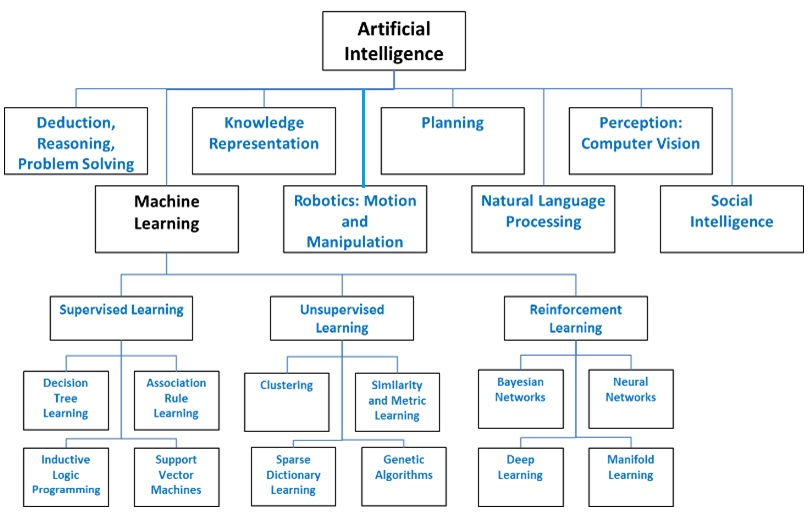
\includegraphics[width=0.7\textwidth]{introduction/images/ai-overview}}
\caption{Dendrogram showing an overview of the field of AI with the position of ML emphasised [source unknown]}
\label{fig:ai-overview}
\end{figure}

\textit{Explainable AI} (xAI) is the sub-field of Artificial Intelligence that ideally should rest at the intersection between Computer Science, Social Sciences and Philosophy and whose aim should be to define the desiderata of artificially intelligent systems and to develop methods to achieve them.
For example, how should a self-driving car behave when confronted with a real-world analogous of the classic Trolley Problem - a situation where each course of action is liable to cause harm?  
On what basis should a person be denied a mortgage, access to university or a job interview?  How can we be sure that there is no bias in the system?  How do we even define if the system is behaving morally?  Would it currently be feasible for a person that feels they have been harmed by such a decision to appeal it?\footnote{For an overview of AI ethics see \citet{Bostrom2011}}
The main idea to achieve these goals is for the systems in question to be somehow made \textit{explainable}. 
The problems start at the very first step, as within the xAI community, as noted by \citet{Doran2018}, there is currently no unanimously agreed upon definition of the definition of \textit{explainability} and consequently of the best way to achieve it in real systems.
The review carried out in Section \ref{sec:explainability} highlights one of the fundamental problems of the field of xAI: that all researchers within the community claim their methods to be \enquote{explainable}, but very few justify this with reasons grounded in the real world (as best noted by the popular paper by \citet{Lipton2016}).

To solve this conundrum various authors have tried to define taxonomies into which classify systems, based on their characteristics and how these relate to its perceived explainability.
One of the most compelling of these is the one proposed by \citet{Doran2018} and shown in Figure \ref{fig:xai-systems-taxonomy}.
The highest level in this classification is taken by \textit{explainable systems} i.e., those that emit explicit, human-understandable reasonings.
This category appears somewhat nebulous in light of the previous paragraph: how should an explainable system be recognised if there is no good definition of explanation?
A less elaborated, but still conceptually sound, taxonomy is the one proposed by \citet{mittelstadt2019explaining} who propose to classify systems based on the source/locus of their explainability.
In this classification models may be \textit{ante-hoc} or \textit{post-hoc} explainable; the former identifies systems whose explainability stems from some internal, inherent characteristic while the latter those whose source of explainability is to be found in some external behaviour, for example the emission of extra symbols.
The two taxonomies are somewhat overlapping even though the latter does not consider \textit{opaque} systems: \textit{interpretable} could be identified with \textit{ante-hoc} while \textit{comprehensible} and \textit{explainable} with \textit{post-hoc}.
A third orthogonal classification by \citet{doshi2017towards} deals with how to \enquote{evaluate an evaluation} of an explanation.
The first two will be presented in more detail in Section \ref{sec:explainability} while the last in Section \ref{sec:evaluation-of-explainability}.

\begin{figure}[htbp]
\centerline{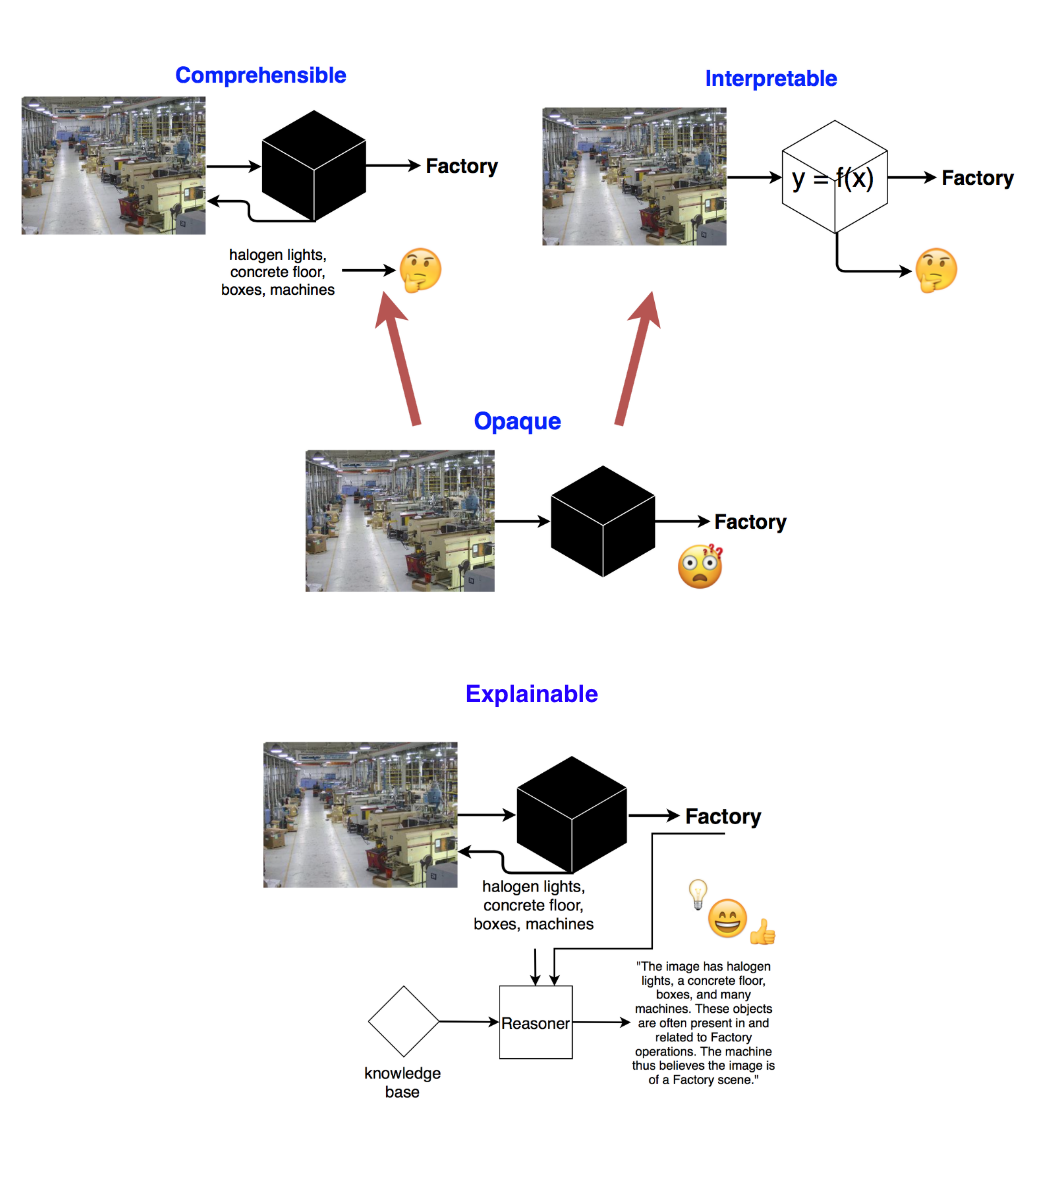
\includegraphics[width=0.9\textwidth]{introduction/images/xai-systems-taxonomy}}
\caption{The relationship between \textit{opaque}, \textit{interpretable},  \textit{comprehensible} and \textit{interpretable} systems [adapted from \citet{Doran2018}]}
\label{fig:xai-systems-taxonomy}
\end{figure}

What I hope can be gleamed from this brief introduction to the field of Explainable Artificial Intelligence, is that many of the problems it aims to tackle are hard \textit{per-se} and may not have a unique optimal solution.  
This is because these issues are not only engineering problems, but exist at the intersection between man and machine and as such can't be tackled using only the methods of Computer Science (this is what is meant by \citet{doshi2017towards} when they talk about \enquote{incompleteness in the problem formalization}).  
This is one of the main pitfalls that the xAI community finds itself falling into, as most of its researchers come from the hard-sciences domains of computer science, mathematics and statistics. 
There is little hope to define the desiderata without the guidance that can only come from philosophy, because of its millennia-long tradition in dealing with ethical issues.  
There is no way to satisfactorily move towards and evaluate these desiderata without resorting to the well-established literature and methods of the Social Sciences (for a good example of how this may work, see \citet{stumpf2009interacting}), as the human element is inherent in any explanation. 
It would be \enquote{reinventing the wheel} to try and define how a computer should relate itself to its user, when the field of Human Computer Interaction has many of these answers already. 
It should be clear that when the human - and particularly the ethical - domain are part of the equation, it is impossible \textit{by definition} to find an optimal and unique solution, that many xAI researchers seem to still regard as achievable.

Effectively, the biggest gap that can be identified is a dearth of explainability methods that have been validated not only with domain experts, but even with real humans.
Many researchers seem content with claiming \textit{formal explainability} and neglect the human half of the explanation.
An explanation, by its nature, involves and \textit{explainer}, the machine, and an \textit{explainee}, us.
Up till now, it seems that xAI is content with \enquote{explaining the explainer}, not realising that in doing so it offers no explanation at all (see \citet{mittelstadt2019explaining} for a critique of the field of xAI, based on this lack of awareness).
\section{Problem and Significance}
The biggest problem of AI is not anymore its perceived usefulness, as this has mostly been solved by its recent successes, but its capacity to elicit the trust of users.
An automated system should be able to make itself be trusted in a manner proportional to the criticality of its application \citep{gilpin2018explaining}, \citep{abdul2018trends}.
The lack of trust that a person may feel, stems from the difficulty in verifying the system's outputs; if no rationale can be inferred for why a given ML model made a certain decision, there is also no way to understand if these outputs conform to our moral norms\footnote{See \citet{gilpin2018explaining} and \citet{abdul2018trends} for a discussion on trust in AI}.
As discussed in Section \ref{sec:importance-of-explainability}, no explicit justification for the link between the explainability and the \textit{trustability} of a model has been found in the reviewed literature; nonetheless, it seems quite natural to infer that a person would not trust decisions made on an unknown rationale. 
Unfortunately, the \textit{explainability} and performance of machine learning models is usually inversely proportional, as is shown in Figure \ref{fig:darpa-comparison-methods}.

There are many examples of modern methods - such as boosted trees, random forests, bagged trees, kernelized-SVMs - that show the tendency outlined in Figure \ref{fig:darpa-comparison-methods}, but this is best exemplified by \textit{deep neural networks} (DNNs). 
Deep Neural Networks are machine learning models constructed by stacking many layers of artificial neurons; these systems are currently offer state of the art performance on a variety of tasks but are among the least easily interpretable systems due to the fact that they represent information in an implicit and distributed manner.  
Some older methods, like decision trees or rule-based methods, are inherently more interpretable due to their simplicity and the fact that they can explicit state their reasoning steps, but are less accurate and flexible than more modern techniques \citep{Biran2017} (as exemplified in Figure \ref{fig:darpa-comparison-methods}).

\begin{figure}[htbp]
\centerline{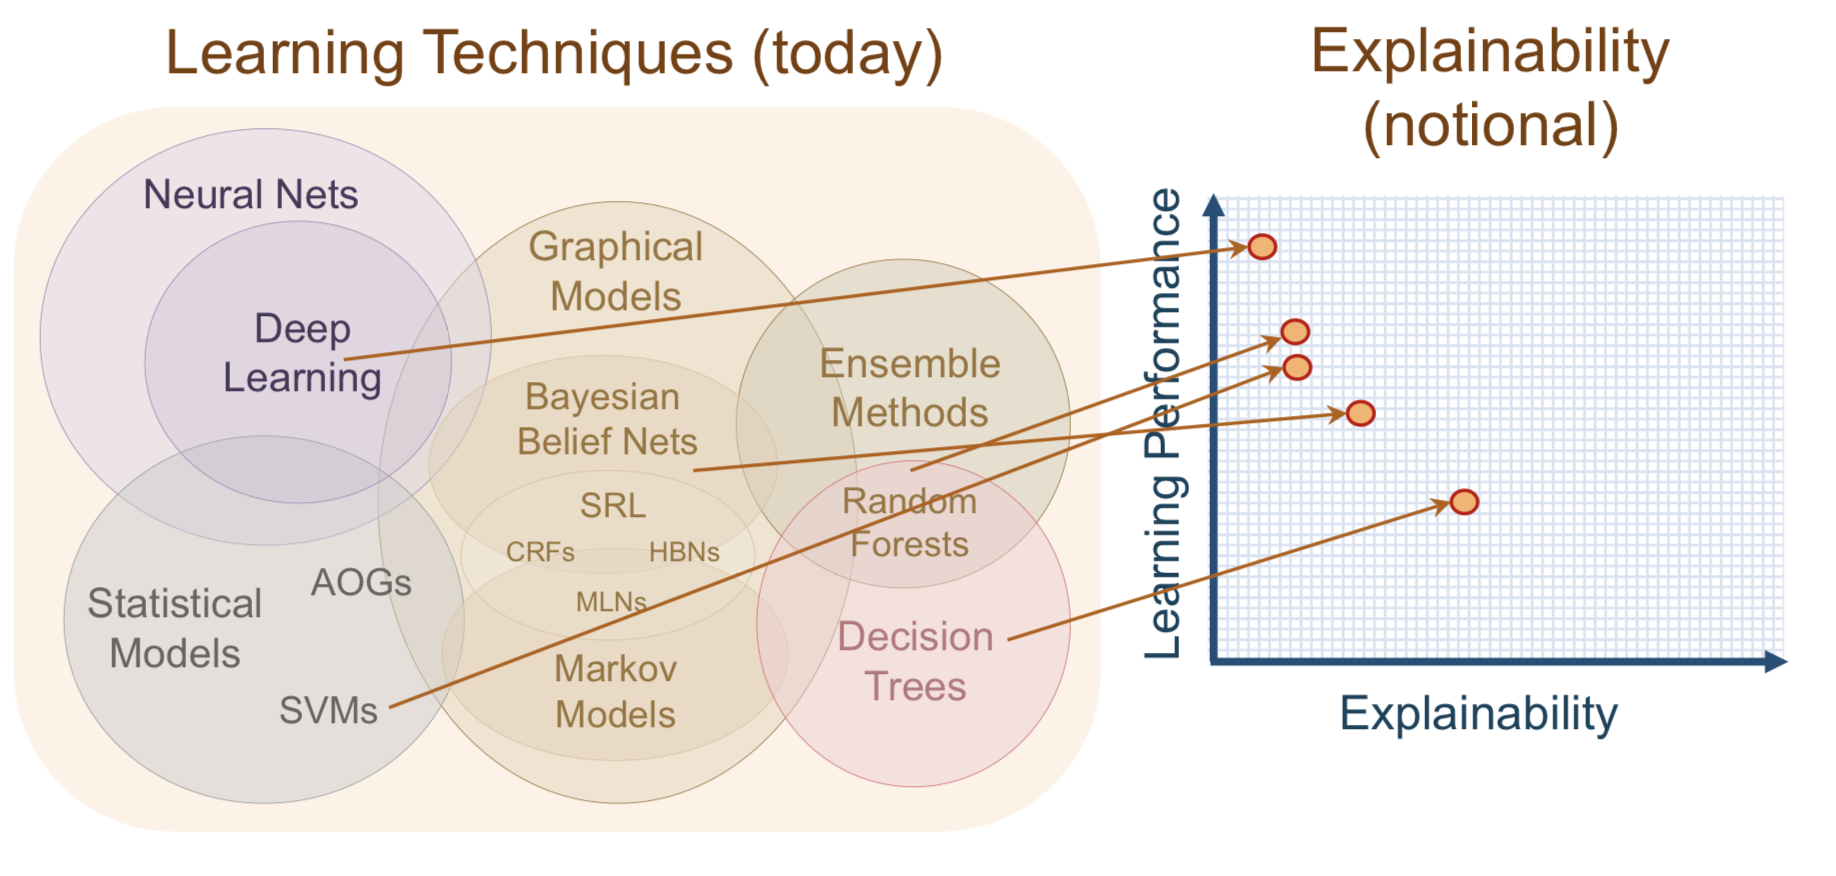
\includegraphics[width=\textwidth]{introduction/images/darpa-comparison-methods}}
\caption{Mapping showing the tradeoff between performance and interpretability of contemporary and older machine learning models \citep{gunning2017explainable}}
\label{fig:darpa-comparison-methods}
\end{figure}

The runaway success obtained by modern Machine Learning in a variety of domains, on a spectrum that goes from engineering to social work, has created the desire to also start applying these methods to mission-critical and traditionally more entrenched fields  (for an overview of deep neural networks as applied to medicine see \citet{Travers2018}).  
A perfect example of an area exhibiting both these characteristics is that of medicine.  
The first successful artificially intelligent systems date back to the 1970s and '80s and were based on \textit{symbolic methods} integrated with \textit{knowledge-bases}.  
These systems were by design capable of providing an explanation for their reasoning and were thus accepted by the medical community in an implementation known as \textit{expert systems}, that aimed to aid in the diagnosis of disease\footnote{For an overview of expert systems see \citet{Liao2005}}. 
The deficiency of modern AI methods in being able to provide causal links for their reasoning process has held back their acceptance in the field of medicine, regardless of their superior performance and accuracy.

One modern ML model that has seen success in the medical domain is that of \textit{Bayesian Networks} (BNs) (defined in much greater detail in Section \ref{sec:bayesiannetworks}), a graphical and computationally efficient way of representing dependencies between variables of interest\footnote{For an overview of BNs in the medical domain see \citet{Lucas2001}}.  
The graphical component is given by the fact that each variable is represented by a node of a Directed Acyclic Graph (DAG) (Definition \ref{def:dag}), with the edges connecting them modelling their dependencies.  
The efficiency stems from the fact that the graph structure imposes a factorisation of the joint probability space and thus lets each variable's values be calculated using only those of its parents.
As is discussed in detail in Section \ref{sec:explainability-in-bayesian-networks}, Bayesian Networks may be uniquely suited to providing effective explanations, by virtue of their inherent characteristics.

In a high-stakes domain such as the medical one, it would be unthinkable for a doctor to trust the predictions of an AI system a priori.
Any decision with profound moral implications - such as prescribing or interrupting the treatment of a patient - would have to first be validated by a human; but, to be able to do so, the clinician would need to be able to understand the rationale behind the machine's output. 
The feasibility of carrying out this validation is dependent on the degree of interpretability of the model that made the decision and, unfortunately, this is the main gap identified in xAI methods.
BNs are no exception, as noted by \cite{timmer2015explaining}, because the underlying formalism makes them appear akin to \enquote{black-boxes} to domain experts who are also not well-versed in statistical reasoning.
Obviously, we don't expect our doctors to also be machine learning experts so the onus of making these models understandable and usable by domain experts falls squarely onto the researchers in the xAI community.
Through a process of real-world validation and testing, they should strive to develop methods that are not only provably correct but, just as importantly, capable of relating efficiently to its intended users.

Explainability is not a necessary condition only for the verification of the system's outputs which, as has just been discussed, is a presupposition for it to be applied in mission-critical domains, but also for the extraction of knowledge from data. 
The amount of information that a machine can process is many orders of magnitude greater than that inspectable by any human; this may let a computer spot new patterns in the data that result undetectable when observing only a moderate amount of samples.   
Being able to understand the mapping from the model's inputs to its outputs, can be seen as understanding the system's \enquote{reasoning} process and could thus lead to knew insights or to the confirmation of existing theories.
This is because understanding the process the model uses to give a certain output can make the machine's analytical power leverageable by our more general/horizontal, but less capable of deep/vertical analysis, capacities.
This is also noted \textit{en passant} by \citet{doshi2017towards} when they state \enquote{humans' goal is to gain knowledge. We do not have a complete way of stating what knowledge is; \textit{thus the best we can do is ask for explanations we can convert into knowledge}}.

In light of all that has been said - that will be explored and justified in much more depth during Chapter \ref{chap:literature-review} - the main focus of this thesis aims to be to address one of the most severe gaps in the current xAI literature: the lack of validation of machine learning systems with real users in real situations.
The work will focus in particular on the medical area and will attempt to evaluate the effectiveness of a Bayesian Network-based system, by an evaluation carried out in collaboration with expert clinical pathologists in a real work setting, over a period of time.
The hope is to validate the current hypothesis that states that Bayesian Networks are inherently apt to being made explainable and also to lay the methodological groundwork for future research aimed at addressing the identified lack of available evaluation in the xAI literature.
\section{Response} \label{sec:response}
In order to contextualise the current work, Chapter \ref{chap:literature-review} will investigate the notions of \textit{explainability}, its importance and how to evaluate it, as defined in the current xAI literature.
In particular, the explainability of Bayesian Networks is reviewed in detail as these will be the basis of the methods carried out in this thesis.

To address the gaps identified in the previous section and in the following chapter, the work carried out in this thesis will concentrate on explainability in the medical domain and will present both a practical part and a theoretical one.
The methods of this thesis will include the implementation of a Bayesian Network-based system, inspired by the work by \citet{Butz2018} (see Section \ref{sec:explaining-the-most-probable-explanation}) and its evaluation.
This paper never provided any results for the compelling method it presents, thus a proof of concept system implementing it together with novel extensions, will be developed.
The system will be a means of exploring the efficacy of the explanatory modes for BNs - as identified by \citet{lacave2002review} - mainly the \textit{graphical}, \textit{verbal} and, in particular, \textit{dialogue}.
Their taxonomy for BN explanations, together with the psychological characteristics  of an explanation \citep{miller2018explanation}, will be the framework against which the methods developed in Chapters \ref{chap:methodology} and evaluated in Chapter \ref{chap:results} will be set.
The explainability of the work will be validated by real medical experts, in a real setting, over a period of time; this will also be a means to provide a validation for the methods of the initial paper \citep{Butz2018} and, more in general, of Bayesian Networks as a whole.
The system will be a proxy to explore the explainability of BNs that should, in theory, be well positioned in being able to give highly effective explanations (as discussed in Section \ref{sec:explainability-in-bayesian-networks}).
The hope is also to set a methodological precedent for other \textit{application-grounded evaluations} (see \citep{doshi2017towards} and Section \ref{sec:evaluation-of-explainability}), with the aim of further reducing the gap of the absence of actual human evaluation of explainability that is present in the xAI literature.

The methodology that will be used to evaluate these hypotheses will start with study of a specific, recent xAI paper by \citet{Butz2018}, whose method will become the basis for the work carried out.
Then a proof of concept system will developed, coded in Python and implementing the learning and updating of a Bayesian Network (see Subsections \ref{subsec:learning-bn-structure}, \ref{subsec:learning-bn-parameters} and \ref{subsec:bnupdating}) together with standard methods (see Subsection \ref{subsec:algorithms}) and novel algorithms (see Subsection \ref{subsec:algorithms-novel}).
The system's main aim will be to support medical decision making through the instauration of a dialogue with the user/domain expert and to evaluate the usefulness, in terms of explainability, of various other interaction modes such as conditional probability and most probable explanation queries (see Subsection \ref{subsec:bnupdating}); various algorithms and interaction paradigms will be developed to do so, as detailed in Section \ref{sec:novel-contributions}.
Finally, this system will be evaluated by expert pathologists at \textit{Istituto Cantonale di Patologia} of Locarno, Ticino, the partner institution which will collaborate on the testing and evaluation of the proof of concept system that will be developed.
The data set that will be used to learn the Bayesian Network, composed by the clinical profiles of over 3000 breast cancer patients in Ticino, will also be contributed by the institute.
The evaluation will be done through the use of interviews, questionnaires and observation of the experts at work, with the objective of clinically validating the system and assess its capacity to relate to the medical professionals in a meaningful manner.

The objective of such a methodology will be to both validate the claims made by \citet{Butz2018} and, more generally, investigate the claims made in the literature regarding the explainability of Bayesian Networks (see Section \ref{sec:explainability-in-bayesian-networks}).
 
%%%%
%%%% LITERATURE REVIEW
%%%%  
\chapter{Literature Review}\label{chap:literature-review}
\section{Introduction} \label{sec:literature-review-introduction}
This chapter aims to carry out a review of recent, relevant literature with the aim of clarifying the main concepts relating to the field of Explainable AI, give a feel of how researchers have approached these and, most importantly, identify current trends and gaps.

The chapter is organised as follows:
\begin{itemize}
  \item Section \ref{sec:explainability} aims to clarify the concept of \textit{explainability}, that is central to the field of Explainable AI and to every further discussion.
  \item Section \ref{sec:importance-of-explainability} investigates the reasons for the importance assigned to explainability in our contemporary societies.
  \item Section \ref{sec:evaluation-of-explainability} is an overview of the main methods that have been proposed to measure explainability.
  \item Section \ref{sec:explainability-in-bayesian-networks} will focus on an assessment of the previous concepts as applied specifically to Bayesian Networks.
  \item Section \ref{sec:explaining-the-most-probable-explanation} offers a review of a recent paper by \citet{Butz2018} and connects it to aforementioned notions.
  The reason for this analysis, is that this paper is an important reference for the work carried out in this thesis as it will be the starting point of the methodology.
\end{itemize}

Throughout the chapter, various gaps that are present in the literature will be identified and assessed; these will be summarised in a coherent fashion in Section \ref{sec:literature-review-summary}.
\section{Explainability} \label{sec:explainability}
\citet{Doran2018}, based on a frequency analysis of explanation terms within documents from relevant research communities, highlight how different circles have different approaches to the concept of explainability and how, even within the same group, terms are used interchangeably.
In particular, they note the overloading of the notion of \enquote{explaination} with that of \enquote{interpretability}; a concept that is often defined within the xAI community as necessary for, but distinct from, explainability.
The use of \enquote{interpretable}, as signifying the property belonging to a system whose inner workings are accessible, can be found, for example, in the recent paper by \citet{gilpin2018explaining}.
In other recent works the two terms are conflated, for example by \citet{mittelstadt2019explaining}, \citet{guidotti2018survey} and in the influential work by \citet{doshi2017towards}.
This seems to prove the point made by \citet{Lipton2016} in the widely-cited paper \enquote{The Mythos of Model Interpretability}, that \enquote{the task of interpretation appears underspecified. Papers provide diverse and sometimes non-overlapping motivations for interpretability, and offer myriad notions of what attributes render models interpretable}.

Most works, even those that blend the notions of interpretability and explainability, seem to agree on the end-goal that implementing such a concept should have; that is, to \enquote{summarize the reasons for neural network behavior, gain the trust of users, or produce insights about the causes of their decisions} \citep{gilpin2018explaining} by being able to \enquote{explain or to present in understandable terms to a human} \citep{doshi2017towards}.
Where the consensus diverges, is in defining what constitutes an explanation and in fixing the desiderata that it may have.
\citet{mittelstadt2019explaining} identify within the literature, two broad classes of interpretability/explainability: \textit{transparency} (also called \textit{ante-hoc} explainabilility) and \textit{post-hoc} interpretability.
The former type deals with the internal workings of a system while the latter applies to its external behaviour.
\citet{Lipton2016} identifies three explanations that can make a model transparent: a mechanistic understanding of the workings of the system in its entirety, of the individual components or of the algorithm.
A system may be made post-hoc interpretable by way of, among others, natural language explanations, visualisations or interactive interfaces.
These methods often do not precisely clarify the exact working of a model, but \enquote{they may nonetheless confer useful information for practitioners and end-users of machine learning}.
\citet{Biran2017} notes how the transparent or \textit{white-box} paradigm was sufficient for classic rule-based models but - with the advent of contemporary machine learning models - is no longer useful.
They argue that it is nowadays unreasonable to expect that any domain expert be able to understand a prediction if they are not also a machine learning specialist.
To address this issue, they propose a Natural Language Generation system; that is, a post-hoc explanation in the categorisation by \citet{mittelstadt2019explaining}.

A widely-recognised feeling, tightly connected with the already recognised lack of shared working definitions, seems to be that researches of Explainable AI are ignoring the enormous corpus of existing models in philosophy, psychology, cognitive and social sciences and human-computer interaction.
This feeling of disconnect is echoed by \citet{gilpin2018explaining} who points out how philosophical texts have long debated what constitutes an explanation, by \citet{mittelstadt2019explaining} who explicitly says how \enquote{many different people, be they lawyers, regulators, machine learning specialists, philosophers, or futurologists, are all prepared to agree on the importance of Explainable AI [...] very few stop to check what they are agreeing to, and to find out what Explainable AI means to other people involved in the discussion}.
The fact that Explainable AI researchers seem to be intent on \enquote{reinventing the wheel} is stated most strongly by \citet{miller2018explanation}, whose paper \enquote{Explanation in Artificial Intelligence: Insights from the Social Sciences} is based on the premiss that \enquote{most of the research and practice in this area seems to use the researchers' intuitions of what constitutes a `good' explanation} and argues for the adoption of the existing research in the social sciences.
The author's views are well summarised by the position xAI is set to occupy in Figure \ref{fig:xai-position}.
The feeling is that Explainable AI researchers are terming their methods \enquote{explanation} based on purely personal views and are thus building explanations that only work for themselves; in other words, \enquote{the inmates are running the asylum} \citep{Miller2017}.
The following quote by \citet{guidotti2018survey} seem to perfectly sum up the state of the research in the field: 
\begin{quotation}
	It is evident that the research activity in this field completely ignored the importance of studying a general and standard formalism for defining an explanation, identifying which are the properties that an explanation should guarantee, e.g., soundness, completeness, compactness and comprehensibility. Concerning this last property, there is no work that seriously addresses the problem of quantifying the grade of comprehensibility of an explanation for humans, although it is of fundamental importance. 
	
	\hfill \citep[pag. 37]{guidotti2018survey}
\end{quotation}

\begin{figure}[htbp]
\centerline{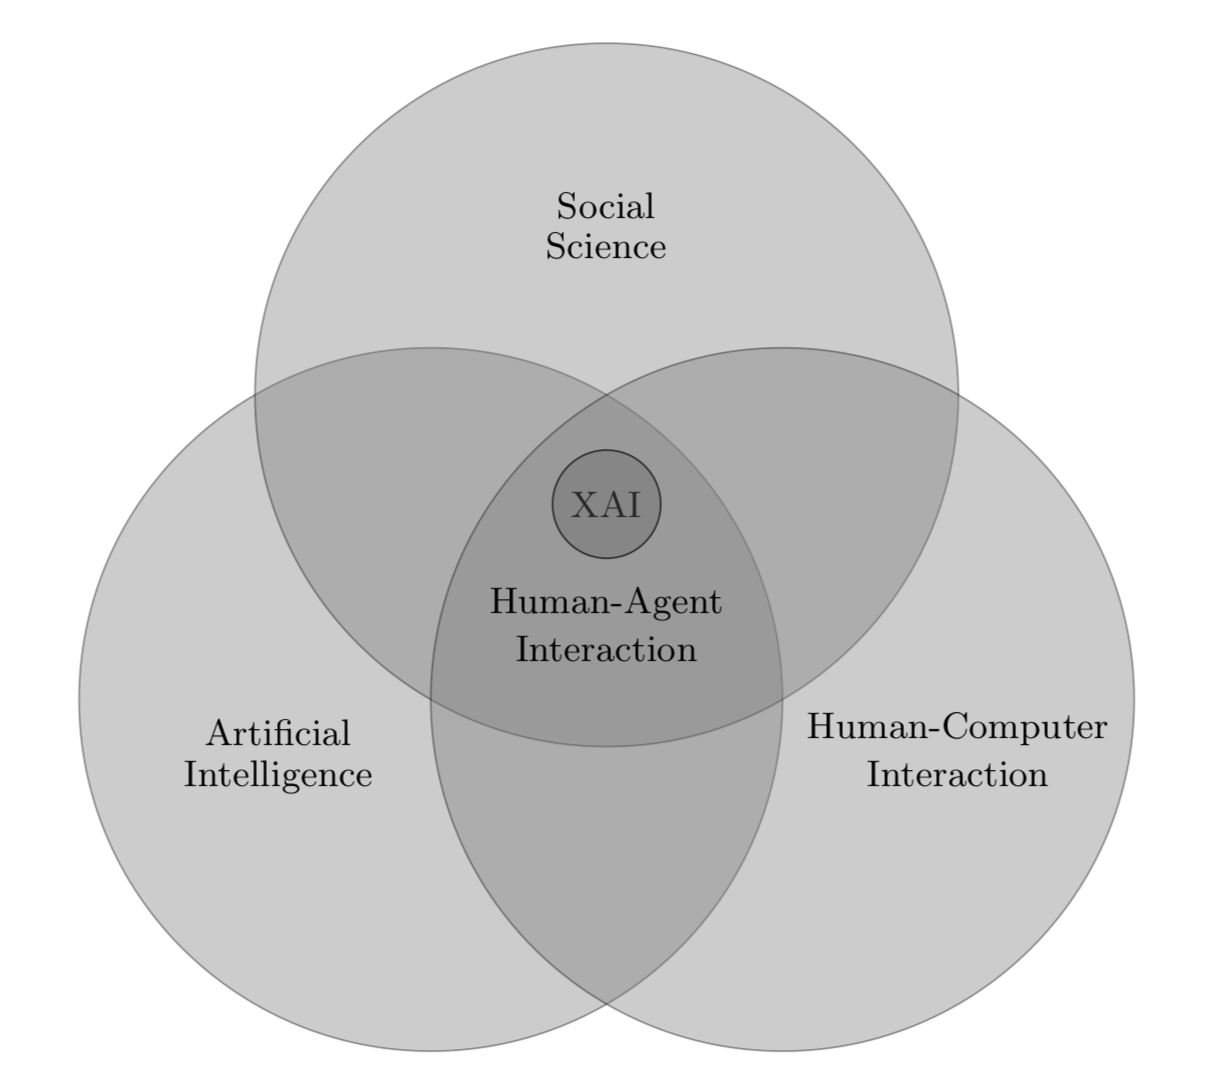
\includegraphics[width=0.5\textwidth]{literature-review/images/xai-position}}
\caption{Venn diagram showing where the field of xAI should \textit{ideally} be positioned \citep{miller2018explanation}}
\label{fig:xai-position}
\end{figure}

To remedy to this state of affairs, there have been a number of works, such as that by \citet{doshi2017towards}, that attempted to define what an explanation means and to reach consensus on it.
The most compelling attempt is in a paper by \citet{Doran2018} (already mentioned in Section \ref{sec:intro-context}) where the authors try to synthesise the current state of affairs into a taxonomy of models:
\begin{itemize}
	\item \textit{Opaque systems}: these are systems that offer no insight into their internal workings that transform the inputs symbols, usually real-world data, into some output, for example labels that classify the data or predictions of unseen cases. 
		All closed-source algorithms fall under this definition.
	\item \textit{Interpretable systems}: this is the vastest category, as the characteristic of these systems is \textit{transparency} i.e., their inner workings are accessible but the onus of comprehensibility falls completely onto the user.  
		The classical example is that of Neural Networks where the mapping from inputs to outputs is inspectable by the user who can, theoretically and depending on her skill, interpret them.
		In the case of Neural Networks this may be a daunting task due to their distributed and non-symbolic nature; in other classes of Machine Learning models, for example Bayesian Networks, the task may be easier as discussed in Section \ref{sec:explainability-in-bayesian-networks}.
	\item \textit{Comprehensible systems}: systems in this category emit additional symbols together with their outputs with the explicit intent of giving the user the means to interpret and understand the automated decisions.
		The additional symbols may be visualisations, natural-language text or any other means of demystifying the output.  
		These extra symbols would need to be graded based on the user's expertise, as comprehension is a property that involves both man and machine.
		An example of such a system would be an image classifier that together with its output also highlighted the parts of the image it used to make its decision.
	\item \textit{Explainable systems}: the highest level in the taxonomy includes those models that emit an explicit \textit{explanation} i.e., a human-understandable line of reasoning.
\end{itemize}
It is recognised that comprensibility depends not only on the system's characteristics, but also on the user's ability and knowledge, thus implicitly accepting the view that xAI should learn from the social sciences.
\textit{Comprensibility} and \textit{interpretability} are considered separate concepts as comprehension requires transparency but interpretation does not, given that the user may reason only over the emitted extra symbols.
This notion of comprensibility is expanded into that of \textit{real} explainability, that is based on a notion of \enquote{ability to formulate, for the user, a line of reasoning that explains the decision making process of a model using human-understandable features of the input data}.

\section{Importance of Explainability} \label{sec:importance-of-explainability}
As noted by \citet{edwards2018enslaving}, \enquote{businesses and governments are increasingly deploying machine learning (ML) systems to make and support decisions that have a crucial impact on everyday life} so, as \citet{gilpin2018explaining} say, \enquote{it becomes necessary for these mechanisms to explain themselves}.
This feeling of urgency and purpose is echoed throughout the reviewed literature; it seems, that even if researchers and the field as a whole cannot agree on a definition of explainability (as discussed in Section \ref{sec:explainability}), there is a keen awareness on the need for models to be explainable.
This intense urge to define explainability and, at the same time, try and create models exhibiting this property, may be counterproductive as the field risks fragmenting into a series of diverging strands, as noted by \citet{abdul2018trends} and visualised in Figure \ref{fig:xai-citation-network}.

\begin{figure}[htbp]
\centerline{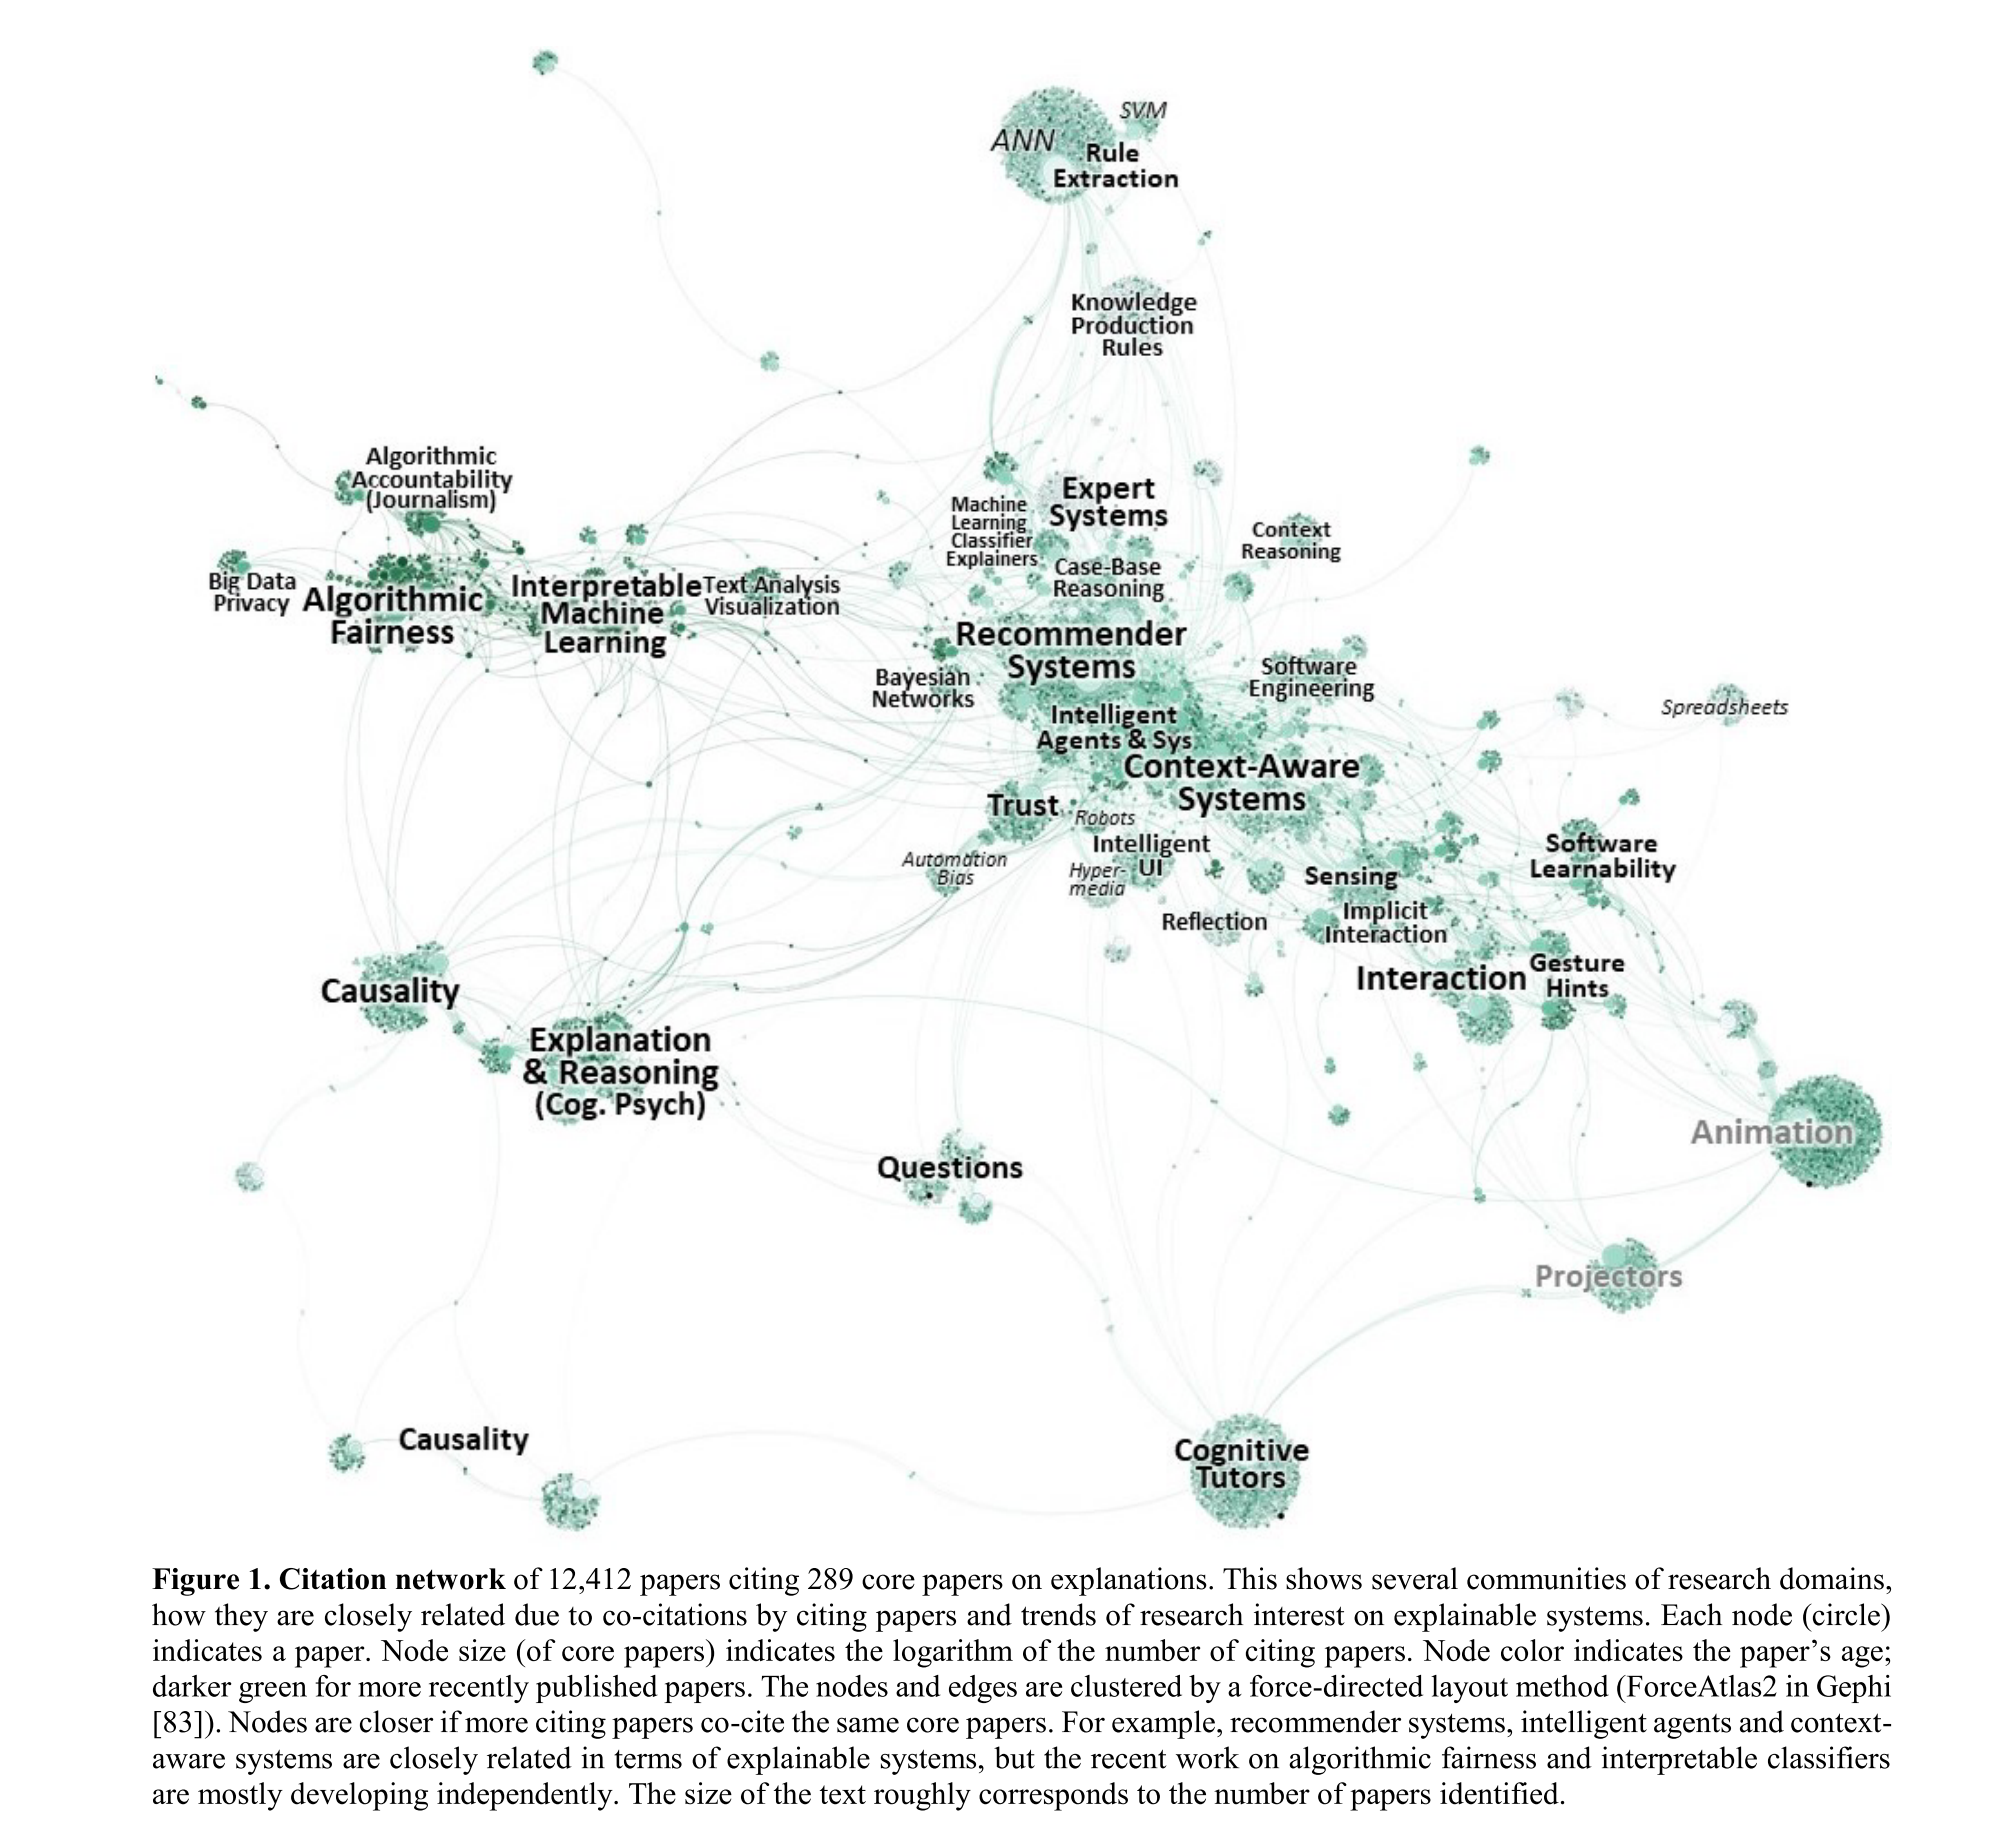
\includegraphics[width=0.8\textwidth]{literature-review/images/xai-citation-network}}
\caption{Citation network that is emblematic in showing the breadth of research strands in the field of xAI \citep{abdul2018trends}}
\label{fig:xai-citation-network}
\end{figure}

There are a myriad of reasons that are brought forth as a justification for the development of Explainable AI, and we will review these in the following paragraphs, but it seems timely to start with one in particular: the need introduced by the European Union's broad General Data Protection Regulation (GDPR).
The GDPR was approved by the European Parliament in 2016 and came into effect in 2018.
More than one author cites an urgency to conform to this regulation (for example \citet{doshi2017towards}, \citet{gilpin2018explaining}), most likely referring to Article 22 of the regulation that, supposedly, mandates for a \enquote{right to an explanation} of algorithms.
While algorithmic explainability is undoubtedly a commendable end-goal, it may be the case that this particular reason to strive for it be a false one.
\citet{edwards2018enslaving} posit that Article 22 of the GDPR actually does not contain the publicised right to an explanation but is \enquote{merely a right to stop processing unless a human is introduced to review the decision on challenge} and as the authors point out, there are, nowadays at least, very few systems without a human in the loop.
Secondly, there is no mandate for the \enquote{explanation} to be human-understandable, so the obtained result may actually be no explanation at all.
If the analysis of \citet{edwards2018enslaving} were correct, then the urgency advocated by many researchers on the grounds of conforming to the GDPR would turn out, in reality, to be based on no valid reason.

A second motive brought forth for the necessity of explainability, for example by \citet{gilpin2018explaining} and \citet{abdul2018trends}, is that comprehensible models are much more likely, or even necessary, to engender users' trust.
While this may very probably be the case, no motives are given for why this should be the purpose of Explainable AI and not just a desirable by-product of obtaining explainability. 
A reasoning for why trust may stem from explainability can be found in \citep{Kyrimi2016} where it is claimed that \enquote{the lack of trust may be due to the difficulty of understanding how a prediction is inferred from the given data. As Aristotle wrote `we do not have knowledge of a thing until we have grasped its why, that is to say, its explanation'. Hence, explaining a model's reasoning - its inference - could increase trustworthiness.} 

Other authors, for example, \citet{doshi2017towards} and \citet{guidotti2018survey}, frame the issue as one of moral necessity.
One need not look far to find examples of ML models displaying covert bias or making decisions we would regard as unethical; a more in-depth investigation would reveal that this was the case even before the popularisation of \enquote{black box} models as are Deep Neural Networks.
\citet{guidotti2018survey} give a reasonably comprehensive list of classic cases that show the risks inherent in not having comprehensible AI.
The oldest of these dates back to the 1970s and 1980s and tells of a system used to screen job applicants that, even though programmed to ignore people's ethnicity, was still seen to discriminate against minorities.
In the same vein but much more recent, the American Military discovered that their computer vision system, that was developed to differentiate between enemy and friendly tanks automatically, had poor accuracy because it had learned to use the background information of the test set photos instead of the pixels representing the actual tanks.
Both these cases exemplify how an algorithm may make \enquote{wrong} inferences based on spurious or latent information that was already in the data set but that no human could have imagined being relevant.
Other failures epitomise how a model may learn our own social prejudices; for example, a recent Princeton study \citep{caliskan2017semantics} proved how models trained on web text corpora showed marked biases (towards race, gender ...) that reflected the ones present in our own society.
Based of their findings, the authors went as far as to suggest that transparency would not be enough to uproot biases, as the very \textit{semantics} of language reflects prejudice latent in our culture. 

The driving motivation and sense of urgency present in all of the reviewed literature is quite certainly tied to the renewed interest and applicability of AI.
\citet{Preece2018} claim that the interest for explainability is naturally linked to that in AI; if this were true, then it would confirm that a need for transparency is implicit in the field itself.
This would validate the assertion made by \citet{doshi2017towards}, that the need for an explanation stems from an \textit{incompleteness in the formalisation}.
What is meant by this is that optimising for certain objectives may introduce an \textit{unquantifiable bias} into the system, that is very different than mere \textit{uncertainty}.
Mere uncertainty can be rigorously quantified, formalised and reasoned upon by using Probability Theory; unquantifiable bias is the result of an \textit{incompleteness in formalisation} of the problem that the ML system is tasked with.
This is the case when a system is coded, for example, to pursue soft-objectives such as \textit{ethics}; such an end-goal may be too abstract and nebulous to be completely formalised.
It might also be the case that a particular objective is far too complex for all its possible outcomes to be exhaustively enumerated.
A good characterisation of objectives leading to incompleteness could be given by applying the concept of \enquote{wicked problem} introduced by \citet{Rittel1973} when analysing the issues arising in social planning.
The first defining characteristic of a wicked problem is that the mere definition of the problem at hand is the wicked problem itself, since even its description is dependent on one's idea for solving it; there is no definite locus that one can point to as the source of the problem. 
Other defining features are the absence of stopping and objective evaluation criteria and the fact that each solution to a wicked problem is essentially \enquote{one-shot} and unique.  
Even the set of possible solutions and causes are not predetermined and non-stationary. 
The authors noticed how these problems presented a series of defining characteristics, that they were able to generalise into the notion of wicked problem.
A classic example are the issues that arise when trying to solve a social planning problem: various parties will have competing objectives and different ideas to obtain them, so no unique best solution is possible; \enquote{at best, they are only re-solved} \citep{Rittel1973}. 
These situations generally tend to arise when dealing with human values, as there is always a degree of ethical relativism that makes it difficult to develop and evaluate solutions.  
\citet{Lipton2016} is also aware of this and states that \enquote{the demand for interpretability arises when there is a mismatch between the formal objectives of supervised learning and the real world costs in a deployment setting}.
In the presence of such unquantifiable uncertainty, that is unavoidable in many of the important applications of AI, requiring the resulting model to be open to inspection would make the \enquote{gaps in problem formalization visible to us} and thus enable us to apply our best human judgement to evaluate them and their consequences \citep{doshi2017towards}.
No wicked problem has a solution that is either true or false, but only good or bad; necessarily, the only judge for this can be a human.

\section{Evaluation of Explainability} \label{sec:evaluation-of-explainability}
As concluded in Section \ref{sec:importance-of-explainability}, the fact that ML models operate on incomplete assumptions makes it a necessity to have some form of evaluation of their performance.
As \citet{Lipton2016} states, \enquote{it turns out that many situations arise when our real world objectives are difficult to encode as simple real-valued functions} and this could lead to evident difficulties in optimising with respect to soft, but of paramount importance, concepts such as ethics and legality.
Being able to evaluate an automated explanation lets us \enquote{serve those objectives that we deem necessary but struggle to model formally}.

Unfortunately, the finding outlined in Section \ref{sec:explainability}, namely there being no consensus on the definition of explainability also necessarily entails that there is no agreed-upon methodology to evaluate such a property.
\citet{doshi2017towards} note as much when they comment \enquote{unfortunately, there is little consensus on what interpretability in machine learning is and how to evaluate it for benchmarking}.
This makes perfect sense because trying to evaluate something without first having defined it, is worse than trying to hit a moving target.
Once again, the feeling among many authors is that \enquote{inmates are running the asylum}.

Some authors have tried to put some order in the barrage of proposed methods; \citet{doshi2017towards} provide one of the most compelling attempts.
These authors set out to outline a taxonomy, having noted a \enquote{lack of rigour} and how current interpretability approaches usually fall into two categories: interpretability in the context of an application and interpretability via a quantifiable proxy.
 The former approach assumes that \enquote{if the system is useful in either a practical application or a simplified version of it, then it must be somehow interpretable}; the latter sees researchers claim that a model class is interpretable and then present algorithms to optimise within that class.
 In their words, both classes rely on a notion of \enquote{you'll know it when you see it}.
 The taxonomy the authors propose is laid out in Figure \ref{fig:xai-taxonomy} and borrows from methods already standard in human-computer interaction and visualisation; the guiding ideal is that \enquote{evaluation of applied work should demonstrate success in the application} and thus the best kind of evaluation is the one that involves humans the most:
 \begin{itemize}
  \item \textit{Functionally-grounded Evaluations}: at the lowest level of their taxonomy are those methods that require no human-in-the-loop and evaluate the explanation quality of a system by using some proxy measure; the advantage is the low cost, but the tradeoff is a lack of specificity.
 A proxy measure that has already been human-validated, for example a decision tree, a set of rules or a linear model \citep{guidotti2018survey} as regards its explainability, may be an appropriate measure for more exotic systems.
 \item \textit{Human-grounded Evaluation}: the second level of evaluation involves humans, albeit not domain expert ones, carrying out simplified versions of the target application; this kind of setup enables the testing of more general notions of explainability.
 \item \textit{Application-grounded evaluation}: this is considered the gold standard evaluation; the authors claim that there is no better way to evaluate explanability that having a domain expert test it in the context of a real task.
In their words, \enquote{the best way to show that the model works is to evaluate it with respect to the task}: \enquote{for example, a visualization for correcting segmentations from microscopy data would be evaluated via user studies on segmentation on the target image task; a homework-hint system is evaluated on whether the student achieves better post-test performance.  Specifically, we evaluate the quality of an explanation in the context of its end-task, such as whether it results in better identification of errors, new facts, or less discrimination}.
\end{itemize}
  
\begin{figure}[htbp]
\centerline{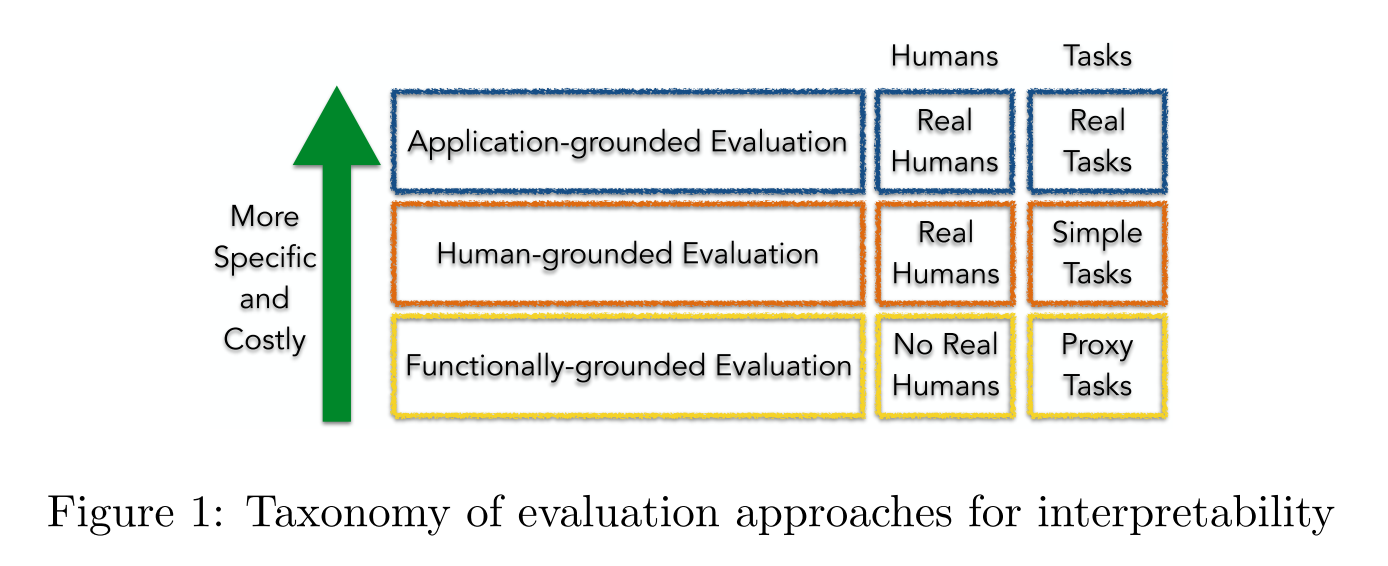
\includegraphics[width=\textwidth]{literature-review/images/xai-taxonomy}}
\caption{Taxonomy of methods for the evaluation of explanations \citep{doshi2017towards}}
\label{fig:xai-taxonomy}
\end{figure}

\citet{guidotti2018survey} outline a taxonomy developed along a different axis; specifically they identify: 
\begin{itemize}
  \item \textit{methods to explain black box models};
  \item \textit{methods to explain black box outcomes};
  \item \textit{methods to inspect black boxes and methods to design transparent boxes}.
\end{itemize}
An essential factor that the authors identify is that \textit{evaluation is a graded notion}; as also noted by \citet{gilpin2018explaining}: different users, with different expertise and background, may rate the quality of the same explanations very differently.
Another point they make - that is quite novel - is that time should also be part of an evaluation; depending on the available time a user may prefer a more straightfoward or more elaborate explanation.
They end by noting that very few works take user expertise and the time taken to understand the proposed explanation into account.

The neglect of the human side of explanations is also lamented by \citet{abdul2018trends} who see researchers focusing on creating mathematically-explainable models at the expense of ones that are usable and practical in real-world situations.
Again, the underlying issue seems to be that xAI researchers are unaware or ignoring the sizeable corpus of research available in cognitive psychology, human-computer interfaces and philosophy.
The authors see the opportunity for HCI to bridge the gap between models and users by way of an interactive approach, as opposed to the mainstream static explanations being proposed in the literature.
An interactive explanation may take the form of a dialogue or of various visualisation techniques; the defining characteristic of such a mode is that it lets the user freely explore the system's behaviour.
\citet{guidotti2018survey}, while discussing the types of data used in ML models, lend credence to the adequacy of this output modality via the statement that \enquote{other forms of data which are very common in daily human life are images and texts. They are perhaps for human brain even more easily understandable than tables}.

\citet{guidotti2018survey}, though, take the view that evaluation of model \textit{comprehensibility} should be equated to its \textit{complexity}, that is not an opinion that often appears in the relevant literature.
Basically, the authors are advocating for the use of complexity - the number of identifiable elements in a particular class of model, for example the number of weights in a neural network or of rules in an expert system - as a proxy for explainability, if we are framing the issue using the taxonomy proposed by \citet{doshi2017towards} (see Figure \ref{fig:xai-taxonomy}).
This may very well be a valid approach, but there is no supporting evidence for it in the paper itself.

A useful reference for how to set up an experiment falling into the class of either human-grounded or application-grounded evaluation, can be found in \citet{stumpf2009interacting}.
In this work the authors set up \enquote{three experiments to understand the potential for rich interactions between users and machine learning systems}; the first, and most relevant, was a think-aloud study that investigated \enquote{how machine learning systems should explain themselves to end users, and what kinds of improvement feedback end users might give to the machine learning systems}.
These studies are interesting as a blueprint for future human-centred evaluations, of the type whose absence is being lamented by many authors.

\citet{mittelstadt2019explaining} summarise the existing critiques to offer a clear and direct evaluation of the field of Explainable AI as a whole, when they state that:
\begin{quotation}
	no matter the approach taken in xAI, reflexivity \textit{[taking account of itself or of the effect of the personality or presence of the researcher on what is being investigated, clarification not by authors]} is needed to ensure the community actually works towards its normative and practical goals to render models holistically transparent or provide high-quality post-hoc interpretations of model behaviour. Critical questions must be repeatedly asked and answered. For example, will the methods developed make machine learning models more interpretable? More trustworthy to users? More accountable? And to whom will explanations be accessible, comprehensible, and useful? Answering such questions requires considering the methods developed in xAI in the context of prior work in fields addressing such normative and social questions. Local and approximation models may in fact resemble existing, well-known approaches to explanations in the `explanation sciences', which would provide insight.
	
	\hfill \citet[pag. 3]{mittelstadt2019explaining}
\end{quotation}

They then conclude by stating that \enquote{xAI generally avoids the challenges of testing and validating approximation models, or fully characterising their domain}.
From the review of the current state-of-the-art carried out in this section and Section \ref{sec:explainability} and \ref{sec:importance-of-explainability}, these could both be seen as entirely valid criticisms.
It really seems that the field of xAI as a whole should try and reposition itself as suggested in Figure \ref{fig:xai-position} and not try to build methods from first principles, many of which may be outside the domain of expertise of the researchers proposing them.

\section{Explainability in Bayesian Networks} \label{sec:explainability-in-bayesian-networks}
Bayesian Networks are a popular class of probabilistic models that has enjoyed widespread appeal as a Machine Learning method, especially inside the medical domain.
The classic \enquote{Asia} toy example of a BN is shown in Figure \ref{fig:asia-bn}; this simple BN is composed of eight nodes and the visualisation makes clear how each one is associated with a \textit{probability distribution} (introduced in Subsection \ref{subsec:probability-interpretations}).
The popularity of BNs in the area of medicine may be because the formalism (see Section \ref{sec:bayesiannetworks}) \enquote{offers a natural way to represent the uncertainties involved in medicine when dealing with diagnosis, treatment selection, planning, and prediction of prognosis. 
This is due to the fact that the influences and probabilistic interactions among variables can be described readily in a BN} \citep{Lucas2001}; that is, even if the BN model is \textit{complete}, in the sense that every possible probabilistic statement can be computed in it, it also is easy to combine multiple variables of interest into composite statements.
Thus, unlike other popular ML algorithms that may have higher learning performance, BNs enable \textit{reasoning} on the model (by, for example, using the algorithms presented in Subsection \ref{subsec:bnupdating}).
Another attractive feature of BNs is their relatedness to the class of \textit{Causal Networks} that were popularised by the groundbreaking work of \citet{Pearl1988}; for all intents and purposes, a Causal Network is simply a Bayesian Network where all the relationships represent a causal effect.
Nonetheless, BNs are not considered as inherently interpretable by the literature, and thus, a series of methods were developed to address this shortcoming.
\citet{timmer2015explaining} note this in the introduction to their paper by stating that \enquote{for non-statistical experts, however, Bayesian networks may be hard to interpret. Especially since the inner workings of Bayesian networks are complicated they may appear as black box models}, \enquote{the interpretation of BNs is a difficult task, especially for domain experts who are not trained in probabilistic reasoning}.

\begin{figure}[htbp]
\centerline{\includegraphics[width=0.8\textwidth]{literature-review/images/asia-bn}}
\caption{Classic example of Bayesian Network \citep{asiabn}}
\label{fig:asia-bn}
\end{figure}

The best overview of the state of explainability of BNs, that will also be used as a framework for the system developed in this thesis, is given by \citet{lacave2002review} in the paper \enquote{A review of explanation methods for Bayesian networks}; here the authors identify various classification criteria for an explanation given by a BN:
\begin{itemize}
  \item \textit{description} vs. \textit{comprehension}: the former consists in displaying the data set or providing further details regarding the output, the latter attempts to guide the user in understanding the model's conclusions.
  \item \textit{micro-level} vs. \textit{macro-level}: detailed description of how a single node in the network is affected vs. showing the main lines of reasoning.
  \item \textit{verbal} vs. \textit{graphical}: \enquote{the most direct and intuitive way of showing the information embodied in a Bayesian network is to display the corresponding graph}.
  When presenting probabilities, \citet{henrion1990qualtitative} strongly suggest that these be \enquote{linguistic probabilities} i.e., for the quantitative probabilities inherent in the model to be converted to a qualitative equivalent.
  This is validated by research showing that linguistic expressions of probability are better understood than the equivalent numerical representation. 
  Some of the many models surveyed in the paper user colours, shading and line thickness to represent the salience of links and nodes.
  The work carried out in this thesis will extensively use both verbal and graphical explanations; the probabilities will also always be linguistic.
\end{itemize}
When compared against the taxonomies already presented in Section \ref{sec:explainability}, it is obvious that these methods applied to a BN, would make it a \textit{comprehensible system} or \textit{post-hoc explainable}.
This is because the model would be emitting extra symbols (graphical, verbal ...) geared towards explaining its outputs.

The authors also identify the three components of BNs that need to be explained: the \textit{knowledge base}, the \textit{model} and the \textit{evidence propagated}.
The first of these \enquote{consists of determining which values of the unobserved variables justify the available evidence} and is, in general, done by finding the solution to the Most Probable Explanation problem (Definition \ref{def:mpe}).
The explanation of the model is considered a static explanation (as opposed to dynamic ones, that will shortly be covered) and is simply the process of verbally or graphically displaying the information already present in the data.
The final element to explain, that is what would most commonly be called an explanation in xAI circles, is the reasoning behind the model's outputs; a system may accomplish this by providing a justification for its outputs, for the results it did not give or via hypothetical reasoning.
The first of these is maybe the most important, because it is paramount for any system, not just a BN, to be able to explain the reasons behind its outputs; returning to the medical setting, it was seen that physicians, in particular, are very reluctant to accept the advice of a machine if they can not understand how it was obtained.
A BN, unlike other ML systems, can also innately exhibit evidence for why it did not provide the output expected by the user and can also reason \textit{counterfactually} i.e. provide alternative outputs.
This will also be an important part of the work carried out in this thesis, as \enquote{counterfactuals} will be used to help medical experts extract knowledge from data. 
The last two capabilities of Bayesian Networks are particularly important, from an explainability perspective, in light of the findings by \citet{miller2018explanation} regarding the nature of explanations that are investigated from a psychological perspective whose conclusions are that explanations possess four primary characteristics:
\begin{itemize}
  \item explanations are \textit{contrastive}: that is people do not ask why an event happened by why another event did not happen instead.  
  A Bayesian Network, as noted in the previous paragraph, is capable of modelling counterfactuals which enables them to give contrastive reasons naturally.
  \item explanations are \textit{selected}: people expect the explanation given to them to have been selected based on some criterion or cognitive bias; they do not expect a complete recount of all causes of an event.
  A BN has the ability to flexibly combine its constituent variables into an output and thus its explanations can be selected based on some criteria or be \textit{partial}, for added simplicity; a BN's outputs needn't be \textit{complete} i.e., constituted of all its parameters, unlike those of non-local models (for example, Neural Networks).
  \item to people, probabilities are not as important and not as well understood as causal relationships.
  BNs, as already mentioned, are closely related to \textit{graphical causal models}, so their explanations have the possibility of being based on causal grounds \citep{Lipton2016}, \citet{rani2006empirical}.
  \item explanations are \textit{social}: that is they involve an \textit{explainer} and an \textit{explainee}.  
  This is recognised in \enquote{Conversational processes and causal explanation} by \citet{Hilton1990}, the most important work on the social aspects of conversation, which supports the view that an \textit{explanation} is a \textit{conversation}. 
  A dialogue is an example of a \textit{dynamical explanation}, in the framework set out by \citet{lacave2002review}; these authors also recognise that an explanation \enquote{always means explaining something to somebody} and thus that \enquote{one of the key features of an effective explanation is the ability to address each user's specific needs and expectations, which primarily depends on the knowledge he/she has}.
  	  So \enquote{In the case of a Bayesian network, the explanation generated for a user that is familiar with the concepts of prevalence, prior/posterior odds and likelihood ratios should be very different from the explanation generated for a user who has never heard about them}.
  	  \citet{lacave2002review} again recognise that explainability is a graded notion but go further and define the concept of \textit{fixed user model}, noting that practically all explainable BN systems have made this assumption and ignored the possibility of users having varying knowledge.
  	  Though, some of the systems surveyed in the paper make a step in that direction by incorporating an \textit{importance threshold} mechanism that would let the user only display certain items; this enables these systems to display varying levels of detail without having defined a defined user model.
\end{itemize}
A dialogue could probably make a BN an example of \textit{explainable system}, in the framework developed by \citet{Doran2018} and \textit{post-hoc explainable system} in that of \citet{mittelstadt2019explaining}.

Bayesian Networks, without any additional explainability methods, would most probably fall into the class of \textit{Interpretable systems}, as do many other ML models, in the taxonomy set forth by \citet{Doran2018}.
Though, based on this review of the literature, it could be suggested, on quite a strong basis, that Bayesian Networks are better equipped than other Machine Learning models to provide a meaningful explanation to humans.
This could be claimed because it is quite widely believed that our brains, and thus our psychology, are near-optimal problem-solvers and as such approximate optimal Bayesian solutions.
A standard view in the fields of psychology and neuroscience, as noted by \citet{Bowers2012}, is that our brain processes approximate the \textit{rational player} as presented in the Dutch Book Argument (see Ch.7 of \citet{anand2009handbook}) and are thus Bayesian in nature.
It is also worth noting that this view has recently been challenged, for example by \citet{Bowers2012}.
This said, even if our brains were not inherently Bayesian, the characteristics of Bayesian Networks make them more capable than other ML models in being able to generate explanations tailored to our cognitive biases and psychology, as discussed in the above bullet points.

% !TEX root = thesis-thomas-tiotto.tex

\section{\enquote{Explaining the Most Probable Explanation}} \label{sec:explaining-the-most-probable-explanation}
The paper \enquote{Explaining the Most Probable Explanation} by \citet{Butz2018} inserts itself into the literature concerned with the explainability of Bayesian Networks.
In particular, taking the classification proposed by \citet{lacave2002review} presented in Section \ref{sec:explainability-in-bayesian-networks}, it attempts to define a \textit{verbal explanation} to the \textit{knowledge base} and of the \textit{propagated evidence}.
Unlike in the definition of explanation of a knowledge base given by \citet{lacave2002review} and of other previous works, the paper is not concerned with finding the most probable assignment of variables that would explain the given evidence but, rather, the inverse problem.
By starting with evidence and finding a maximally probable configuration, the authors hope \enquote{to look at the complete scenario to get an overview before deciding which variables should be focused on}; that is, the goal appears to give the user an overview of the situation.  

The initial claim of the paper is that BNs, even though they provide a graphical structure to the knowledge base, remain of difficult interpretation for domain experts.
The examples brought to justify the claim are that edges in the graph do not necessarily represent causal dependencies and that d-separation (Definition \ref{def:d-separation}) may be confusing.
The authors plan to address this claim by constructing a \textit{dialogue} with the user and thus to continue in the long tradition of dialogical approaches to explaining BNs.

The defining characteristic of their approach is that the domain expert is able to \enquote{argue} with the MPE and investigate alternative explanations.
The complete methodology, that is executed over three steps, is shown in Figure \ref{fig:butz-methodology}.
The first step is the construction of the \enquote{knowledge base}, which is nothing else than a probability tree representing a \enquote{chain of deduction} constructed following the strongest probabilistic dependencies between variables in the BN.
Such a knowledge base is convenient because the document plan for the Natural Language Generation step is directly derived from it.
One issue that is immediately apparent is that this greedy approach does not \enquote{generate the MPE solution} as the authors claim.
This does not discredit the argumentative method as a whole, as it is not necessary for the user to be arguing the MPE to derive a good explanation; this ties into one of the main findings in the previous sections that many xAI researchers are only focusing on half of what an explanation is.
A good explanation is not given only by its formal properties but, most importantly, by how it acts as an interface between the real \textit{user} and the model.
This is what \citet{abdul2018trends} mean when they lament that \enquote{despite their mathematical rigour, these works \textit{[referring to the existing explainability methods]} suffer from a lack of usability, practical interpretability and efficacy on real users}.

\begin{figure}[htbp]
\centerline{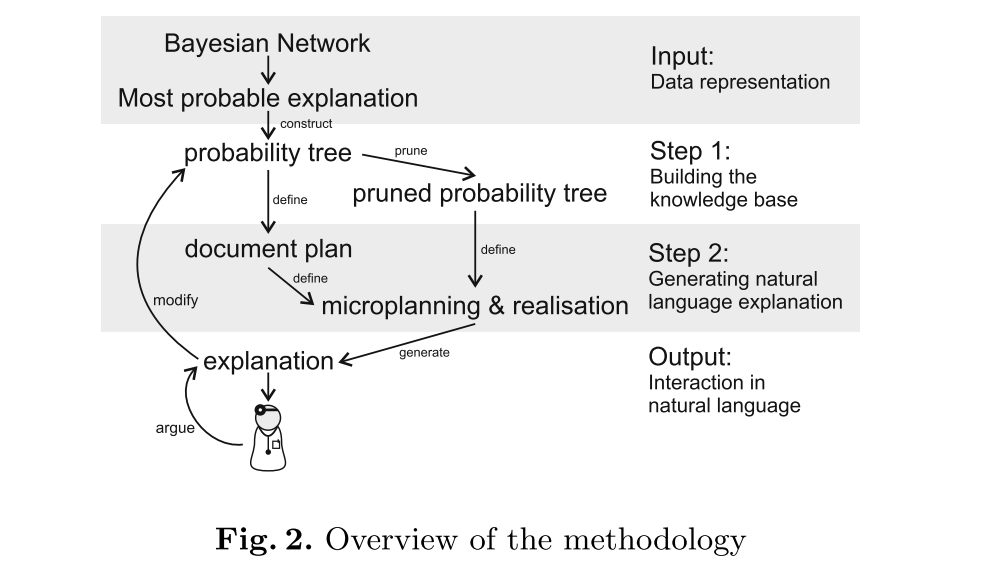
\includegraphics[width=\textwidth]{literature-review/images/butz-methodology}}
\caption{Overview of methodology followed by \citet{Butz2018}}
\label{fig:butz-methodology}
\end{figure}

The document plan for the argumentation follows the same chain of strongest dependencies constructed in the knowledge base until the expert disagrees; at that point, the user is presented with an alternative \enquote{MPE}.
An example of how the document plan may look after interaction with the user is shown in Figure \ref{fig:butz-tree}.
All the natural language phrasing is generated via boilerplates that take care of realising both the micro-planning phase and the generation of the text.

\begin{figure}[htbp]
\centerline{
\includegraphics[width=\textwidth]{literature-review/images/butz-tree}}
\caption{\textit{Document plan} generated from the \textit{probability tree} \citep{Butz2018}}
\label{fig:butz-tree}
\end{figure}

The authors recognise that such chains of deduction could become long and cognitively overloading in the case of larger BNs, as every variable in the tree is explained by all its ancestors.
A solution they propose is that of \textit{pruning} the probability tree by excluding d-separated nodes and those under a certain threshold of significance.
They also adapt some methods from literature to perform \textit{conflict analysis}; that is, only variables that contribute positively to the explanation are maintained in the document plan.

On the whole, \citet{Butz2018} offer a compelling explanation method for BNs by building on an established tradition of explainability through dialogue.
The work, though, takes some methodological missteps and also continues the \enquote{sin} of not validating its claims on real users, one of the primary gaps in the xAI field identified in the previous sections.
\section{Summary} \label{sec:literature-review-summary}
The findings outlined in this chapter refer to the concept of explainability of Machine Learning models, to its importance, to ways of evaluating it and to explainability in the specific case of Bayesian Networks.
The concept of explainability is central to the field of Explainable AI (xAI), whose goal is to make Machine Learning systems \enquote{interpretable}.
Explainability can briefly be defined as the property of a system that is able to \enquote{explain or to present in understandable terms to a human} \citep{dosilovic2018} its outputs.
Two main classes of explainable models have been identified by \citet{mittelstadt2019explaining}: ante-hoc or transparent and post-hoc interpretable ones; the formers are inherently inspectable in their inner workings while the latters are made understandable by way of extra techniques.
These two classes have also been refined by \citet{doshi2017towards} into a four-tier taxonomy consisting of: \textit{opaque}, \textit{interpretable}, \textit{comprehensible} and \textit{explainable systems}.
An opaque system, also know as a \enquote{black-box model}, is one whose inner workings are not inspectable from the outside; an interpretable system corresponds to an ante-hoc interpretable one; a comprehensible one emits extra information together with its output; an explainable system explicitly outputs a human-understandable line of reasoning aimed at clarifying its workings.

Explainability has become a central concept to the field of AI as a whole; as ML models take over more and more functions in our societies, the pressure for them to be able to explain their decisions is increased accordingly.
The \textit{General Data Protection Regulation} (GDPR) that became effective in 2018 was viewed by many as increasing the societal pressure to make systems explainable; many may have been mistaken as regards the actual rules mandated by the regulation - that aren't really prescribing a broad \enquote{right to an explanation} \citep{edwards2018enslaving} - but nonetheless the feeling of urgency is sure to increase the focus of both researchers and laypeople.
In general, explainability is framed as an issue of moral necessity as it easy to find a long series of situations where ML models displayed covert bias or what we would regard as bad moral judgement.

There are all manner of ways to measure explainability and these can be classified into a three-layer taxonomy \citep{doshi2017towards} based on the assumption that the best type of evaluation is the one that most involves humans.
The three classes are \textit{functionally-grounded evaluation}, \textit{human-grounded evaluation} and \textit{application-grounded evaluation}, ordered from the one least involving real humans to the one where the presence of the human-in-the-loop is greatest.
As the involvement of humans in evaluating models' explanations increases, so does the cost of such an experiment and its specificity, as the highest evaluation level necessarily entails the collaboration of domain-experts on specific tasks.
A parallel taxonomy identifies: methods to explain black box models, methods to explain black box outcomes, methods to inspect black boxes and methods to design transparent boxes.
An overarching notion that has been stressed is that \textit{explainability is a graded notion} that depends on the knowledge and expertise of the particular user: different users, with different expertises and backgrounds, may rate the quality of a same explanation very differently.

Bayesian Networks (BNs) have enjoyed widespread appeal in mission-critical domains like that of medicine and thus the drive to develop methods to explain their outputs has always been strong.
BNs have three main elements that necessitate an explanation \citep{lacave2002review}: the \textit{knowledge base}, the \textit{reasoning process} and the \textit{evidence propagated}.
Explaining the first \enquote{consists of determining which values of the unobserved variables justify the available evidence} and is done by solving the Most Probable Explanation (MPE) problem.
For the second, a static explanation of the BN is achieved by displaying it graphically or verbally.
The last element is explained by showing the reasoning that brought the BN to give the outputs it did that can be achieved by providing a justification for its outputs, for the results it did not give or via hypothetical reasoning.
The fact that BNs are able to naturally support counterfactual reasoning, combine single variables into composite outputs and model causality puts them at an advantage compared to other ML systems when generating an effective explanation for a user.
This is because the capabilities of a BN enable it to generate explanations that are uniquely suited to out psychological biases and expectations of what an explanation should entail.

Some of the main gaps that were found during the review of the literature relate to how there is still a great confusion in the field of xAI regarding what an explanation really is and thus what constitutes a good instance of it.
There is also a prevalent methodological confusion, as different authors use terms in incongruous ways, for example sometimes \textit{intepretation} is taken to mean \textit{explanation} while in other cases they refer to different concepts, for example in the taxonomy of interpretable systems proposed by \citet{doshi2017towards}.
This naturally makes it difficult for the field to converge onto methods to evaluate such explanations and this is reflected in the barrage of methods present in the literature, each one focused only on a particular system or instance of model.
This confusion is exacerbated by a seeming lack of interest or awareness of xAI researchers for the sizeable corpus of work in psychology, philosophy, social sciences, neuroscience and human computer interaction that has already investigated the nature of explanations, what desiderata they may possess and which are most effective.
In fact, the great majority of proposed approaches is only focused on proving formal explainability and neglects the human side that is naturally present in any explanation; there has been little work carried out to validate approaches in real settings with real domain experts so many explainability methods are substantiated only at theoretical level.
The underlying issue that has been seen to run transversely across the various concepts investigated in this chapter is best summarised by the idea that \enquote{inmates are running the asylum}, meaning that individual researchers are claiming that their models are interpretable referring only to their own personal views and biases and not to established literature and methods.
It would be hard for them to do otherwise, as the field of xAI seems, at present, to be a collection of diverging strands without a comprehensive program able to help it converge onto its stated goal: to make Machine Learning systems understandable by their users and thus increase their social utility and acceptance.


%%%%
%%%% MATHEMATICAL BACKGROUND
%%%%
\chapter{Mathematical Background}\label{chap:mathematical-background}
\section{Introduction} \label{sec:mathematical-background-introduction}
This chapter will arrive to give a formal definition of Bayesian Networks, a class of Probabilistic Graphical Models that are used to represent systems under conditions of uncertainty.

The chapter is organised as follows:
\begin{itemize}
  \item Section \ref{sec:probability-theory} introduces a series of basic concepts from Probability Theory focusing mainly on the basic concept of random variables and also establishing the notions of conditioning, independency and correlation.
  \item Section \ref{sec:information-theory} presents information entropy and uses it to define measures for random variables, \textit{Kullback-Leibler divergence}, and distance measures for other objects, \textit{Hamming and Jaccard distances}.
  \item Section \ref{sec:graph-theory} introduces the objects of graphs and polytrees and the central concept of \textit{d-separation}.
  \item Section \ref{sec:bayesiannetworks} uses the content of the previous sections to define the Bayesian Network formalism and then gives an overview of structure learning algorithms and the notions of \textit{conditional probability and maximum a posteriori queries}.
\end{itemize}

Not all the concepts introduced in this chapter are strictly needed for the description of the Bayesian Network formalism, but all will be useful as a mathematical reference for the methods developed in later chapters of this thesis.
\section{Probability Theory} \label{sec:probability-theory}
We will be dealing with \textit{standard probability} so random variables and probability measures will always be real-valued.
We will also, in the work carried out in this thesis, only be considering the case of random variables that can assume a finite number of possible values/states.
We will refer to these variables as \textit{categorical} to indicate that there is no natural ordering among their states.

\subsection{Random Variables} \label{subsec:random-variables}
\begin{definition}[Event]
	Given $\mathcal{S}$ the space of all possible outcomes of interest, an event $\sigma$ is a subset of $\mathcal{S}$: $\sigma \subseteq \mathcal{S}$.
	
	$\mathcal{F} \subseteq 2^{\mathcal{S}}$ is the set of all events that are under consideration.
	
	Two events $\sigma$ and $\tau$ are called disjoint when $\sigma \cap \tau = \emptyset$.
\end{definition}

\begin{definition}[Random Variable]
	A random variable $X$ is a function $X: \mathcal{S} \rightarrow \mathcal{X} \subseteq \mathbb{R}$ that associates every outcome $s \in \mathcal{S}$ with a value.
\end{definition}

\textit{Random variables} are a way of bringing to the fore the attributes of interest of events while dealing with them in a clean, mathematical way.
The values that a random variable can take are a function of the events in sample space $\mathcal{S}$, with each of these having a value assigned by the random variable function.

\begin{definition}[Probability Measure] \label{def:probability-measure}
	Given a sample space $\mathcal{S}$ and events $\mathcal{F}$, a discrete probability measure $\mathbb{P}$ is a function $\mathbb{P}: \mathcal{F} \rightarrow [0,1]$ that assigns a probability value to every event. 
	In the discrete case all subsets of $\mathcal{S}$ can be treated as events thus $\mathcal{F}$ is the power set of $\mathcal{S}$.
To be a valid probability measure, $\mathbb{P}$ must satisfy:
\begin{itemize}
	\item $\mathbb{P}(\mathcal{S}) = 1$;
	\item If events $\sigma$ and $\tau$ are disjoint then $\mathbb{P}(\sigma \cup \tau)=\mathbb{P}(\sigma)+\mathbb{P}(\tau)$.
\end{itemize}
\end{definition}
Each event $\sigma \in \mathcal{F}$ must have a probability $\mathbb{P}(\sigma) \in [0,1]$ and the sum of all these must equal $1$. 
An event with $\mathbb{P}(\sigma) = 0$ is deemed \textit{impossible} while one with $\mathbb{P}(\sigma) = 1$ is \textit{certain}.

\begin{definition}[Probability Mass Function]\label{def:mass-function}
	A probability mass function of a discrete random variable $X$ is a function $f_X: \mathcal{X} \rightarrow [0,1]$ defined, using a probability measure $\mathbb{P}$, as:
\begin{equation*}
	f_X(x) = \mathbb{P}(\{s \in \mathcal{S} : X(s)=x\}) \,,
\end{equation*}
and thus assigns a probability to every value $x \in \mathcal{X}$ in the domain of $X$.
\end{definition}
The probability mass function returns the probability of a random variable $X$ taking on exactly its value $x$.
This probability is the size of the subset of the event space $\mathcal{S}$ whose events $s$ are mapped to $x$ by the random variable function $X$.

Every random variable has a probability distribution induced by the cardinality of the subsets of its values; in the case of discrete one, such a distribution is \textit{multinomial}.

Often, in the context of random variables the probability distribution $f_X$ is called the \textit{marginal of $X$} and is usually contrasted with the notion of \textit{joint probability distribution}.
\begin{definition}[Joint Probability Mass Function]
	The joint probability mass function of discrete random variables $X$ and $Y$ is a function $f_{XY} : \mathcal{X} \times \mathcal{Y} \rightarrow [0,1]$ defined as:
	\begin{equation*}
		f_{XY}(x,y) = \mathbb{P}( \{s \in \mathcal{S} : X(s)=x \} \cap \{ s \in \mathcal{S} : Y(s)=y\} ) \,,
	\end{equation*}
	and thus assigns a probability to every tuple $(x,y)$ with $x \in \mathcal{X}$, $y \in \mathcal{Y}$.
\end{definition}

In what follows, we will sometimes refer to the marginal probability $f_X$ of $X$ as $\mathbb{P}(X)$, to $f_X(x)$ as $\mathbb{P}(X = x)$, to joint probability $f_{XY}$ of $X$ and $Y$ as $\mathbb{P}(X,Y)$, and to $f_{XY}(x,y)$ as $\mathbb{P}(X=x,Y=y)$ as the only random variables we will be dealing with will be discrete.
Notice that the notation $(E = e)$ is also often overloaded to signify an assignment of values to a set of random variables $E$; in this case what is meant is that every variable in the set $E = {X_1,...,X_k}$ assumes a certain value from its own domain. 
We will denote sets in bold so $\boldsymbol{E} = \boldsymbol{e}$ stands to mean that every variable $E$ in the set of random variables $\boldsymbol{E}$ assumes a value $e$ from its own domain. 
Finally, recall that the set of values that $X$ can take is denoted by the cursive $\mathcal{X}$.

\subsection{Probability interpretations} \label{subsec:probability-interpretations}
There are two main views through which to interpret the probability of an event: the \textit{frequentist} and the \textit{subjectivist/Bayesian} one.

The former views the probability of an event as the expected ratio of times it would occur over a great number of trials.
That is, the probability of an event is seen as the \textit{limiting frequency} of a repeatable event.
So, for example, the probability of observing heads when tossing a coin is said to be $0.5$ because over repeated throws heads was observed half the time.

The other view is the subjectivist or \textit{Bayesian} one (from the 18th century mathematician Thomas Bayes) in which probabilities are instead viewed as the \textit{subjective} degree of belief attributable to the manifestation of an event.
In this interpretation, stating that a coin has probability of heads of $0.5$ simply means that the person making the claim personally believes that the chances of seeing heads or tails are the same.
This is useful in that it enables the characterisation of certain events that haven't yet come about or that are liable to happen only once or a small number of times (that is, they are not repeatable).

Philosophically, Bayesian inference assigns a probability to a hypothesis (a \textit{prior}) while the frequentist method tests a raw hypothesis empirically before assigning it any probability.
As Bayesian inference naturally embraces and deals with uncertainty, it is an enormously useful tool to model and reason about the real, stochastic world we live in.

From the Bayesian point of view, we would consider the probability of a state of a random variable as simply representing the subjective degree of belief we would have over a set of outcomes we believed could manifest themselves.

\subsection{Conditional Probabilities} \label{subsec:conditional-probabilities}
\begin{definition}[Conditional Probability] \label{def:conditional-probability}
	The conditional probability mass function of random variable $Y$ given $X=x$, $x \in \mathcal{X}$, $y \in \mathcal{Y}$ is:
\begin{equation*}
\mathbb{P}(Y=y \mid X=x) = \frac{\mathbb{P}(X=x,Y=y)}{\mathbb{P}(X=x)} \,.
\end{equation*}
To be defined, it must be that $\mathbb{P}(X=x) > 0$.
\end{definition}

Definition \ref{def:conditional-probability} can easily be manipulated in order to obtain another basic result, called the \textit{chain rule of conditional probabilities}:
\begin{equation} \label{eq:chainrule}
	\mathbb{P}(Y=y,X=x) = \mathbb{P}(Y=y \mid X=x) \mathbb{P}(X=x) \,.
\end{equation}
Equation \ref{eq:chainrule} can be generalised to any number of variables:
\begin{align} \label{eq:chainrule-multiple}
\begin{split}
	\mathbb{P}(X_1=x_1, \ldots , X_n=x_n ) = & \mathbb{P}(X_n=x_n \mid X_1=x_1, \ldots, X_{n-1}=x_{n-1}) \times \\
	&  \ldots   \\
	 &\times \mathbb{P}(X_1=x_1 \mid X_2=x_2 ) \; \times \\
	 &\times \mathbb{P}(X_1=x_1) \,.
\end{split}
\end{align}
Intuitively, it means that we can decompose joint probabilities as products of conditional probabilities.  

Another immediate, and crucial, consequence of Definition \ref{def:conditional-probability} is known as \textit{Bayes' Theorem}, which lets us calculate the revised probability of an event given new knowledge regarding another event.
\begin{theorem}[Bayes' Theorem] \label{th:bayes-theorem}
	Given random variables $X$, $Y$ and the events $X=x$, $Y=y$, $\mathbb{P}(Y=y) > 0$, it holds that:
	\begin{equation*}
		\mathbb{P}(X=x \mid Y=y)=\frac{\mathbb{P}(Y=y \mid X=x) \mathbb{P}(X=x)}{\mathbb{P}(Y=y)} \,.
	\end{equation*}
\end{theorem}
Intuitively, this is a process of \textit{belief revision} as the belief in event $X=x$ is revised by the new knowledge that $Y=y$. 

\subsection{Independence} \label{subsec:independence}
\begin{definition}[Random Variables Independence]
	Two random variables $X$ and $Y$ with domains $\mathcal{X}$ and $\mathcal{Y}$ are independent when their joint probability mass $\mathbb{P}(X,Y)$ is equal to the product of their probability densities:
	\begin{equation*}
		\mathbb{P}(X=x,Y=y) =  \mathbb{P}(X=x) \times \mathbb{P}(Y=y) \quad \forall x \in \mathcal{X}, \forall y \in \mathcal{Y} \,.
	\end{equation*}
\end{definition}
In the real world it is hard or even impossible - if we consider Nature being based on chaos theory when viewed at a fine-enough level - to find two such perfectly non-interacting events.
Thus, a more useful concept is that of \textit{conditional independence} where two previously dependent events become independent when conditioned on a third one

\begin{definition}[Random Variables Conditional Independence]
	Two random variables $X$ and $Y$ with domains $\mathcal{X}$ and $\mathcal{Y}$ are conditionally independent on a third random variable $Z$ with domain $\mathcal{Z}$ when their probability densities conditioned on $Z$ are independent.
	That is, when the joint probability mass function conditioned on $Z$ is equal to the product of the conditional probability mass functions:
	\begin{equation*}
		\mathbb{P}(X=x,Y=y \mid Z=z) = \mathbb{P}(X=x \mid Z=z) \times \mathbb{P}(Y=y \mid Z=z) \quad \forall x \in \mathcal{X}, \forall y \in \mathcal{Y}, \forall z \in \mathcal{Z} \,.
	\end{equation*}
\end{definition}
Intuitively, this means that knowing any value of $Z$ makes the probability distributions of $X$ and $Y$ independent.
\section{Information Theory} \label{sec:information-theory}
The birth of the field of \textit{information theory} is usually traced back to the seminal paper \enquote{A Mathematical Theory of Communication} (\cite{Shannon1949}) where Claude Shannon set the mathematical basis for the quantification of the amount of \textit{information} transmissible over a noisy channel. 
In his words \enquote{The fundamental problem of communication is that of reproducing at one point, either exactly or approximately, a message selected at another point.}
The concepts of field are broad enough to have influenced practically every other scientific discipline and deep enough to have enabled the \enquote{digital age}, for example by enabling the creation of ever more complicated coding schemes for the compression, reconstruction and obfuscation of digital data.

\subsection{Entropy} \label{subsec:entropy}
In classical mechanical statistics, entropy can be seen as a measure of the uncertainty, or randomness, of a physical system.  
This concept was reapplied by Shannon to measure the amount of randomness in a random variable.
\begin{definition}
	Given a random variable $X$ with probability distribution $\mathbb{P}(X)$, its entropy $\Eta(X)$ is defined as the expected amount of information content carried by $X$ (\cite{Schneider2005}):
\begin{equation} \label{eq:entropy}
	\Eta(X) = \mathbb{E}(I(X)) = \mathbb{E}(-\log (\mathbb{P}(X)) = -\sum_{i=1}^{n} \mathrm{P}\left(x_{i}\right) \log _{b} \mathrm{P}\left(x_{i}\right)
\end{equation}
\end{definition}
The base $b$ of the logarithm defines the unit of measure.  Shannon used $b=2$ as he was dealing with the transmission of digital, binary-coded data; in this case the unit of measure are $bits$.

The simplest example of how information entropy characterises a random variable $X$, is in imagining $X$ to model a coin and the task being to predict the probability of the outcome of a throw being heads.
If the coin is fair, we will not be any more surprised to see the outcome being heads than tails; the entropy is maximum as there is maximum uncertainty regarding the outcome.
However, if the coin is not fair and tails is more probable the we will be more surprised than not to see the outcome being heads.  
The entropy is sub-maximal because there is less uncertainty regarding the outcome: tails is more probable than heads.
If one of the outcomes is impossible, for example if the coin has two heads, then the entropy of the coin is $0$ as there is no uncertainty regarding the result of a toss.


\subsection{Normalised Entropy} \label{subsec:normalised-entropy}
Plain entropy is not a good choice when trying to characterise random variables with different cardinalities of their sample space.
Let us suppose that the objective is to find the variable with the least \enquote{entropic} distribution and we suppose that their values have all been generated by the same process, say Gaussian.
Simply calculating their entropies and ordering them according to this criterion will bias the selection process towards the variables with smallest cardinality.
This is because we supposed them to be distributed in the same way so there will naturally be less uncertainty when there are fewer possible outcomes.
This can easily be understood by imagining the distributions to all be random uniform.

To obviate to this problem we need to \textit{normalise} the entropy so that different-sized variables can be directly compared to each other.
To achieve this, we can look at a measure of \textit{normalised entropy} or \textit{efficiency}:
\begin{equation} \label{eq:normalisedentropy}
 	\eta(X)=-\sum_{i=1}^{n} \frac{p\left(x_{i}\right) \log _{b}\left(p\left(x_{i}\right)\right)}{\log _{b}(n)}
\end{equation}
From Eq. \ref{eq:normalisedentropy} it can be seen that $\eta(X) \in [0,1]$; it is thus normalised and comparable among distributions.
This ratio expresses the amount of entropy found in the distribution compared to the maximum possible entropy when using $n$ symbols, corresponding to the uniform distribution:
\begin{equation}
\mathrm{H}\left(\underbrace{\frac{1}{n}, \ldots, \frac{1}{n}}_{n}\right) = - \sum_{i=1}^n \frac{1}{n} \log _{b} \left( \frac{1}{n} \right) = -n \cdot \frac{1}{n} \log _{b} \left( \frac{1}{n} \right) = - \log _{b} \left( \frac{1}{n} \right) = \log _{b}(n) 
\end{equation}   

\subsection{Mutual Information} \label{subsec:mutualinformation}
Another way of characterising the interrelatedness of two variables is through the concept of \textit{mutual information}, as defined in \cite{Cover2006}, that is closely linked to entropy (Eq. \ref{eq:entropy}).
\begin{definition}
	The mutual information of two random variables $X$ and $Y$ is given by:
	\begin{equation} \label{eq:mutual-information}
		I(X,Y) = \sum_{x \in \mathcal{X}} \sum_{y \in \mathcal{Y}} p_{XY}(x,y) \log \left( \frac{p_{XY}(x, y)}{p_{X}(x) p_{Y}(y)} \right)
	\end{equation}
\end{definition}
NB: In Information Theory, the convention is that $0 \log(0) = 0$.

$I_{XY}$, intuitively, measures the amount of information that $X$ and $Y$ share that can also be seen as the degree to which one variable is informative of the other.
If $X$ and $Y$ are independent then they share no mutual information and knowing one of the two gives no information about the other.
This can be immediately understood by rewriting Eq. \ref{eq:mutual-information} as:
\begin{equation}
	I(X,Y) = H(X) - H(X|Y) = H(Y) - H(Y|X)
\end{equation}
The mutual information I(X,Y) is the reduction in uncertainty of one of the variables given the knowledge of the other.
if $X$ and $Y$ are perfectly correlated ($\rho_{XY}= \pm 1$) then they both convey the same amount of information and $I_{XY}$ is equal to the entropy $\Eta(X) = \Eta(Y)$.

\subsection{Hamming Distance} \label{subsec:hamming-distance}
The \textit{Hamming Distance} is a widely-used distance measure that quantifies the similarity of strings.
\begin{definition}
	The Hamming Distance $d_H(x,y)$ between two vectors $x$ and $y$ is given by:
	\begin{equation}
		d_H(x,y) = \sum_i \Gamma(x_i, y_i)
	\end{equation}
	with $\Gamma(i,j)$ defined as:
	\begin{equation}
		\Gamma(i,j) = 
		\begin{cases}
			0 \quad i \neq j \\
			1 \quad i = j	
		\end{cases}
	\end{equation}
\end{definition}
Given strings of characters, or more in general vectors over some field, of equal length, their Hamming Distance is the number of positions where they differ.
It can be seen as the number of substitutions needed to transform one into the other.

This is a valid distance measure because:
\begin{itemize}
  \item it is non-negative: $d_H(x,y) \geq 0 \quad \forall x, y$
  \item it fulfils the identity of indiscernibles: $x = y \Rightarrow d_H(x,y)=0$
  \item it respects the \textit{Triangle Inequality}: $d_H(x,y) \leq d_h(x,z) + d_H(z,y) $
\end{itemize}

For example, strings $x=01234$ and $y=15244$ have $d_H(x,y)=2$, as they differ in two positions.

\subsection{Jaccard Distance} \label{subsec:jaccard-distance}
The \textit{Jaccard Distance} is a popular metric to measure the similarity of sets.
\begin{definition}
	The Jaccard Similarity Coefficient $J(A,B)$ of two sets $A$ and $B$ is given by:
	\begin{equation}
		J(A,B) = \frac{|A \cap B |}{| A \cup B |}
	\end{equation}
\end{definition}
\begin{definition}
	The Jaccard Distance $d_J(A,B)$ between two sets $A$ and $B$ is given by:
	\begin{equation}
		d_J(A,B) = 1 - J(A,B)
	\end{equation}
\end{definition}

This is a valid distance measure because:
\begin{itemize}
  \item it is non-negative: $d_J(A,B) \geq 0 \quad \forall A, B$
  \item it fulfils the identity of indiscernibles: $A = B \Rightarrow d_J(A,B)=0$
  \item it respects the \textit{Triangle Inequality}: $d_J(A,B) \leq d_J(A,C) + d_J(C,B) $
\end{itemize}

For example, the sets $A = \{ 0, 2, 3, 4, 1 \}$ and $B = \{ 1, 3, 5 \}$ have $d_J(A,B) = \frac{2}{6}$, as their intersection is of cardinality 2 and their union of cardinality 6.

\section{Graph Theory} \label{sec:graph-theory}
Many problems in machine learning do not involve classification or prediction of single data points in isolation, but of sets of entities that may present a more, or less, complex relation with each other. 
Most real-world phenomena fit into the latter framework.
Graphs are one of the most powerful tools for the modelling of this class of problems, as their structure naturally captures the wide variety of relations that may exist between entities.
These range from the atomic structure of a molecule to a social network of friends.  
In all these examples graphs help in reasoning, visualising and making inferences and predictions.

\subsection{Directed Graphs} \label{subsec:graphs}
\begin{definition}[Directed Graph]
	A directed graph is a tuple 
	\begin{equation*}
		\mathcal{G} = (\mathcal{V}, \mathcal{E}) \,,
	\end{equation*}
with $\mathcal{V} = \{ v_1 \ldots v_n \}$ the set of vertices/nodes and $\mathcal{E}\subseteq \mathcal{V} \times \mathcal{V}$ the set of edges.
\end{definition}
We will not be concerned with the subclass known as \textit{undirected graphs} that are characterised by $\mathcal{E}$ being a \textit{set} of unordered pairs; that is, of sets of the form $\{x,y\}$, with $x,y \in \mathcal{V}$.

The class of graphs which interest us at present are those where there can be at most a single directed edge between any pair of nodes in $\mathcal{V}$; that is, we are not considering \textit{multigraphs}.
We are also interested in enforcing that there be no \textit{cycles} in the graph so there can be no subset of edges in $\mathcal{E}$ that when followed starting from vertex $v_i$ eventually ends up in $v_i$ again.
A cycle is a \textit{walk} - a sequence of edges which joins a sequence of vertices - of nodes of the form $v_i, v_j, \cdots, v_i$ i.e., a walk where only the first and last vertex are repeated.
Thus we have also automatically excluded the special case of cycle called \textit{self-loop}: an edge from a node to itself. 
The resulting graph possessing only directed edges and no cycles is commonly called a \textit{directed acyclic graph}, or DAG for short.  
\begin{definition}[Directed Acyclic Graph] \label{def:dag}
	A directed acyclic graph is a graph where every edge is directed and there are no cycles.
\end{definition}

In a DAG we may qualify nodes based on their \enquote{relationship status}:
\begin{description}
	\item[children] the children of node $u$ are all nodes $k$ for which there is a \textit{directed edge} from $u$ to $k$;
	\item[parents] the parents of node $u$ are all nodes $k$ for which there is a \textit{directed edge} from $k$ to $u$;
	\item[descendants] the descendants of node $u$ are all nodes $k$ for which there is a \textit{directed path} i.e., a walk where all vertices are distinct, from $u$ to $k$;
	\item[ancestors] the ancestors of $u$ are all nodes for which there is a directed path from $k$ to $u$.
\end{description}
An example of a DAG, containing five nodes, is shown in Figure \ref{fig:bn-example-dag}.

\begin{figure}[htbp]
\centerline{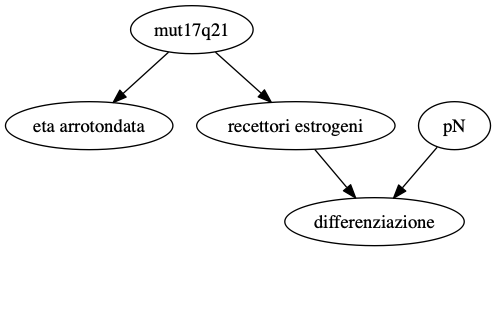
\includegraphics[width=0.5\textwidth]{mathematical-background/images/bn-example-structure}}
\caption{Example DAG representing a subset of the data set used in this thesis.}
\label{fig:bn-example-dag}
\end{figure}

Polytrees and trees will also be defined because these are fundamental concepts for the work carried out in this thesis.
\begin{definition}[Tree] \label{def:tree}
	A tree is an undirected graph where there is one and only one walk between every node.	
\end{definition}
\begin{definition}[Polytree] \label{def:polytree}
	A polytree is a DAG whose underlying undirected graph is a tree.
	That is, if the directionality of edges is removed from the DAG, the resulting object is a tree. 
\end{definition}

\subsection{D-separation} \label{subsec:d-separation}
\textit{Dependence-separation} or \textit{d-separation}, as the name entails, is a concept relating to the conditional dependence between variables and was first presented by \citet{Pearl1988}.
We define the notation $u \rightarrow v$ to signify that there is a \textit{trail} between $u$ and $v$ in the graph, with a trail $(u, \ldots ,v)$ being a walk where all edges are distinct.

$u$ and $v$ and a node $z$ may be arranged in the graph in one of the following four configurations, called \textit{v-structures} in this context:
\begin{itemize}
  \item \textit{chain}: $u \rightarrow z \rightarrow v$
  \item \textit{chain}: $u \leftarrow z \leftarrow v$
  \item \textit{fork}: $u \leftarrow z \rightarrow v$
  \item \textit{collider}: $u \rightarrow z \leftarrow v$
\end{itemize}

We say that these v-structures are \textit{closed} by the set $Z$ when:
\begin{itemize}
  \item \textit{chain}: $u \rightarrow z \rightarrow v$ and $z \in Z$
  \item \textit{chain}: $u \leftarrow z \leftarrow v$ and $z \in Z$
  \item \textit{fork}: $u \leftarrow z \rightarrow v$ and $z \in Z$
  \item \textit{collider}: $u \rightarrow z \leftarrow v$ and $z \notin Z$ and no descendant $z'$ of $z$ i.e., $z'$ such that $z \rightarrow z'$ exists, is also in the set $Z$
\end{itemize}

We say that $u$ and $v$ are \textit{d-separated} by $Z$ if every v-structure they appear in is closed by $Z$.
Conversely, if there is at least one \textit{open} v-structure then $u$ and $v$ are \textit{d-connected}.

If $u$ and $v$ are d-connected, then knowing something about $u$ also tells us something new about $v$, and viceversa.
An intuition for this can be given by interpreting the paths \textit{causally}.
In the case of a \textit{chain}, $z$ is the cause of $v$ so knowing $z$ tells us everything we need to know about the value of $v$ (or of $u$, if the chain is reversed).
In a \textit{fork}, conditioning on the \textit{common cause} $z$ has the same effect: $z$ is sufficient to know $u$ and $v$.
This is also called the \enquote{Common Cause Principle} \citep{sober1988principle}.

A good intuition for the behaviour of \textit{colliders} was given by \citet{Pearl1988}: imagine that there are two independent causes for a car refusing to start ($z$): having no gas ($u$) and having a dead battery ($v$): $u \rightarrow z \leftarrow  v$.
Only knowing that the battery is charged gives no information about the car having fuel or not.
But if we now know that the battery is charged after observing that the car won't start, we know for sure that it must be out of fuel.
So knowing something about $u$ is informative about $v$, after conditioning on $z$.

\begin{definition}[D-Separation] \label{def:d-separation}
	Given vertices $u$ and $v$ and a set of vertices $Z$, then $u$ and $v$ are d-separated by $Z$ if:
	\begin{itemize}
		\item $Z \neq \emptyset$ and $u$ and $v$ are never part of a collider;
		\item $Z = \emptyset$ and $u$ and $v$ are always part of a collider.
	\end{itemize}
\end{definition}

The independencies between variables are encoded in the structure of the DAG so every probability distribution modelled by a BN that has the same connections between nodes, also necessarily has the same independencies regardless of the values of the variables.

A series of examples using the DAG presented in Figure \ref{fig:bn-example-dag} are shown in Figures \ref{fig:bn-separations-example-1}, \ref{fig:bn-separations-example-2}, \ref{fig:bn-separations-example-3}.
We can see how the network's topology and the nodes chosen to be in the observed set $Z$, define the resulting separations.
In all cases $u=$\enquote{eta arrotondata} and $Y=V \mysetminus u \mysetminus Z$; we are asking for the set of all nodes in the DAG that are d-separated from $u$, given evidence $Z$.
This can easily be answered by enumerating all the v-structures in the network and applying Definition \ref{def:d-separation}.
In the case shown in Figure \ref{fig:bn-separations-example-1} we see that the node \enquote{eta arrotondata} is separated from nodes \enquote{recettori estrogeni}, \enquote{differenziazione} and \enquote{pN} given the observed evidence \enquote{mut17q21}.
The reason for this is because \enquote{eta arrotondata} $\leftarrow$ \enquote{mut17q21} $\rightarrow$ \enquote{recettori estrogeni} is a \textit{fork} and thus the flow of information from the rest of the network is blocked.
The way in which changing the conditioning set $Z$ also changes the independencies, can clearly be seen by comparing Figures \ref{fig:bn-separations-example-2} and \ref{fig:bn-separations-example-3}.

\begin{figure}[htbp]
\centerline{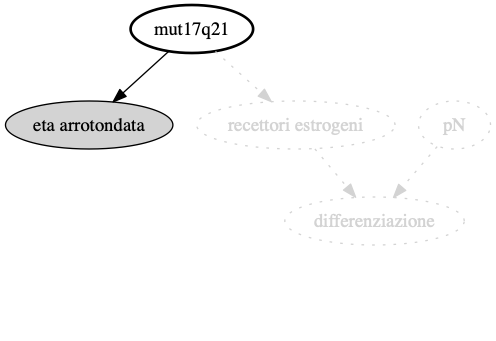
\includegraphics[width=0.5\textwidth]{mathematical-background/images/bn-example-separations-1}}
\caption{D-Separations in a subset of the provided data set (see Section \ref{sec:data-set}).}
\label{fig:bn-separations-example-1}
\end{figure}

\begin{figure}[htbp]
\centerline{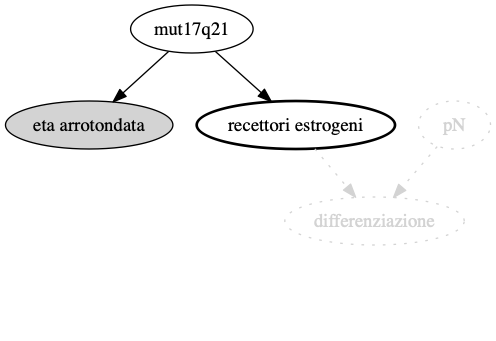
\includegraphics[width=0.5\textwidth]{mathematical-background/images/bn-example-separations-2}}
\caption{D-Separations in a subset of the provided data set (see Section \ref{sec:data-set}).}
\label{fig:bn-separations-example-2}
\end{figure}

\begin{figure}[htbp]
\centerline{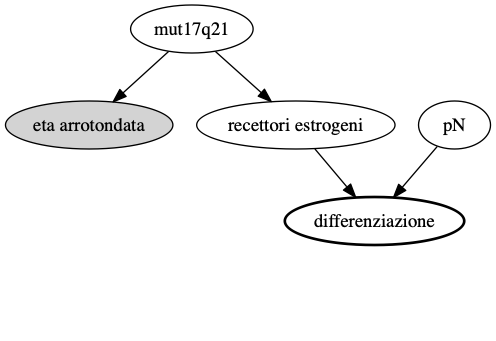
\includegraphics[width=0.5\textwidth]{mathematical-background/images/bn-example-separations-3}}
\caption{D-Separations in a subset of the provided data set (see Section \ref{sec:data-set}).}
\label{fig:bn-separations-example-3}
\end{figure}

\section{Bayesian Networks} \label{sec:bayesiannetworks}
\begin{definition}
	A Bayesian Network (BN) is a probabilistic graphical model represented by a DAG where each vertex corresponds to a random variable $X_i$ and the edges model the dependencies among these.
\end{definition}
Such a model is basically a way of compactly representing an explicit joint distribution $\mathbb{P}(X_1 \cap \ldots \cap X_n) = \mathbb{P}(X_1) \ldots \mathbb{P}(X_n)$, that is factorised into $\mathbb{P}(X_n \mid X_1 \cap \ldots \cap X_{n-1}) \ldots \mathbb{P}(X_2 \mid X_1 ) \mathbb{P}(X_1) $.
The way this compactness is achieved is in exploiting the independencies that exist among the random variables:
\begin{equation} \label{eq:bnindependencies}
	\forall X_i:  ( X_i \perp \neg Desc(X_i) \mid Pa(X_i))
\end{equation}
with $Pa(X_i)$ the set of nodes that are parents of $X_i$ and $Desc(X_i)$ the nodes that are not \textit{descendents} of $X_i$.
That is to say, every random variable $X_i$, given its parent nodes, is independent of all other nodes in the Bayesian Network that are not descended from it.
Also, a BN gives the flexibility to drop the many weak dependencies that are bound to exist between variables thus leading to an even simpler model.
A full probability table for a joint distribution of random variables obscures the independencies and requires an exponential number of entries for the representation.
A Bayesian Network on the other hand can represent the same distribution using only a linear number of parameters.
The way that Bayesian Networks can be used to reduce the storage requirements for uncertain information is by taking advantage of the conditional independencies embedded in the underlying distribution being modelled.
The power of BNs comes from the additional information encoded in their structure and this was first explicitly described in its entirety by \cite{Pearl1988} who defined the concept of dependence separation (see Subsec. \ref{subsec:d-separation}) and applied it to Bayesian Networks.

One nice characteristic of BNs is that they very naturally model the type of mixed causal and stochastic processes that we find in all of Nature.
Imagine we want to represent the process modelled by joint distribution $\mathbb{P}(B,A) = \mathbb{P}(B) \mathbb{P}(A)$; using the chain rule for conditional probabilities (Eq. \ref{eq:chainrule}) we can write this as $\mathbb{P}(B \mid A) \mathbb{P}(A)$.
A BN modelling this process would be composed of two nodes $A$ and $B$ with an edge from the former to the latter $A \rightarrow B$, $A$ is called the ``parent'' of $B$.  Each of these two nodes would have its own probability table, with $\mathbb{P}(A)$ representing the \textit{prior} distribution over $A$ and $\mathbb{P}(B \mid A)$ the \textit{conditional probability distribution} of $B$ given $A$.

We can now see why these types of models are named \textit{Bayesian} Networks: the inference process is based in a given prior distribution/belief and evolves through a parent $\rightarrow$ child relationship to constantly yield an updated \textit{posterior} belief.
The BN DAG encodes a generative sampling where each variable's value is determined stochastically by Nature, based on the value of its parents.
This process is also highly compatible with our view of causality and this is one of the reason that makes BNs highly interpretable.
The prior $\mathbb{P}(A)$ can be seen as the result of some stochastic process caused by a series of latent (unmodelled) variables while the posterior $\mathbb{P}(B \mid A)$ is stochastically, causally determined by $A$. 
As I have mentioned in the previous paragraphs, there are probably no truly ``prior'' distributions in the Universe, at the modelling scale we are usually interested in.
Only on arriving on the quantum particle level may we find ``pure'' stochastic, uncaused processes due to quantum collapse.

A good example of how BNs are well compatible with our notion of causality may be to imagine $A$ as the random variable modelling the predisposition to having a certain disease and $B$ to actually developing the symptoms for it.
\textit{First}, genetic and epigenetic factors such as the environment stochastically contributed to having the predisposition and \textit{then} the development of the symptoms was stochastically determined by the degree of predisposition.
Adding an extra time dimension certainly helps us in dealing with this class of models.

The example show in Fig. \ref{fig:bn-example-dag} is the underlying graph structure of a Bayesian Network, each node is now representing a Random Variable with an associated \textit{Conditional Probability Table} (CPD), that defines its probability distribution, conditional on its parents.
The CPDs for \textbf{eta arrotondata} and \textbf{mut17q21} in the Bayesian Network in question are shown in Tab. \ref{tab:mut-cpd} and \ref{tab:eta-cpd}.
\textbf{Mut17q21} is a root node, i.e. has no parents, in the DAG so its probability distribution is unconditional or \textit{marginal}.
\textbf{Eta arrotondata}, on the other hand, is a child of \textbf{mut17q21} so the probability of its values is conditional on that of its parent.
For example, \textbf{eta arrotondata} takes on value \enquote{<40} $44\%$ of the time when \textbf{mut17q21} has value \enquote{mut}, but only $4\%$ of the time when \textbf{mut17q21} has value \enquote{unknown}.

\begin{table*}[htbp]
\centering
\caption{\textbf{mut17q21} CPT}
\begin{tabularx}{\textwidth/2}{cXX}
\toprule
& mut & unknown    \\ 
\textbf{mut17q21} & 0.006 & 0.99  \\
\bottomrule
\end{tabularx}
\label{tab:mut-cpd}
\end{table*}

\begin{table*}[htbp]
\centering
\caption{\textbf{eta arrotondata} CPD}
\begin{tabularx}{\textwidth/2}{ccXX}
\toprule
      & &  \multicolumn{2}{c}{\textbf{mut17q21}} \\
\cmidrule(lr){3-4}
 & & mut & unknown    \\ 
 \multirow{3}{*}{\textbf{eta arr.}}  & <40 & 0.42 & 0.04  \\
 & 40-50 & 0.42 & 0.17    \\
 & >50 & 0.15 & 0.78 \\
\bottomrule
\end{tabularx}
\label{tab:eta-cpd}
\end{table*}

\subsection{Bayesian Networks Structure Learning} \label{subsec:bnstructurelearning} 
In many probabilistic models initialisation is fast but then fitting the data is slow (ex. k-means).
For Bayesian Networks the converse is true: fitting is fast as only sums of the counts in the data are needed but identifying the correct graph structure can take super-exponential time.
Learning the Bayesian Network structure from data is commonly known as the Bayesian Network Structure Learning (BNSL) problem.
The methods to solve this problem can be roughly categorised into one of three types.

\subsubsection{Search and Score}
This is the most na{\"i}ve method as it does a brute force search over all the possibile graph structure space - i.e. all DAGs with the same number of variables as the input data - and scores all these depending on some cost function.
This process is super-exponential but though the use of dynamic programming and heuristic search algorithms it can become sub-exponential.
Nonetheless, solving the exact BNSL is only feasible up to $~ 30$ variables.

\subsubsection{Constraint Learning}
Methods of this type calculate some measure of correlation to identify the presence and direction of edges between nodes.
A typical test is to iterate over all triplets while testing for conditional independencies.
Thanks to the d-separation properties outlined in Subsec. \ref{sec:bayesiannetworks}, this test is able to identify the correct edges.
The algorithm is quadratic in time in the number of vertices.

\subsubsection{Approximations}
Several heuristical approaches have been developed to be able to find good network structures in an efficient manner.
Examples of these are:
\begin{itemize}
  \item Chow-Liu, that builds a tree approximation of the probability distribution
  \item Greedy Hill-Climbing, that adds/removes/flips an edge at a time
  \item Optimal Reinsertion, that iteratively calculates the optimal $Markov blanket$ (the subset of all nodes that are sufficient to determine the value of another subset) of an ever-smaller subset of nodes
\end{itemize}

\subsection{Bayesian Networks Updating} \label{subsec:bnupdating}
All the types of inference presented are instances of \textit{diagnostic reasoning}, also known as \textit{abductive reasoning}.  
This type of explanation can either be modelled as a conditional probability or a MAP query and is of fundamental importance in many important problems of machine learning including medical diagnosis, that is of particular interest to us.

\subsubsection{Conditional Probability Query}
The \textit{updating} problem is the process of updating the probabilities of nodes in the BN based on the observation of the values of other vertices.
This process of conditioning on observed information is also called \textit{data propagation}.

The following algorithm was described by \cite{Normand1992} and applies to our case where the random variables follow a multinomial distribution.
What we want, is to calculate the conditioned probability $\mathbb{P}(B \mid D)$ i.e. the updated probability of node $B$ based on observed evidence $E$.
\begin{definition}
	The conditional probability query for variable $B$ given evidence $E$ is:
\begin{equation} \label{eq:bnupdating}
	\mathbb{P}(B \mid E) = \alpha \pi(B) \lambda(B)
\end{equation}
with $\pi(B) \lambda(B)$ analogous to the \textit{prior} and \textit{likelihood} of $B$, respectively.
\end{definition}
The likelihood of $B$ depends only on the weighted likelihoods of its children $C_1, \ldots ,C_k$:\begin{align}
	\lambda(B) = \prod_l \lambda_{C_l}(B) \\
	\lambda_{C_{l}}(B)=\sum_{C_{l}} \lambda\left(C_{l}\right) P\left(C_{l} \mid B\right)
\end{align}
and its prior similarly depends only on the information received from its parents $A$:
\begin{align}
	\pi(B)=\sum_{A} P(B \mid A) \pi_{B}(A) \\
	\pi_{B}(A)=\alpha \pi(A) \prod_{S_{B}} \lambda_{S_{B}}(A)
\end{align}
The information is propagated down if any variable observed is above $B$ while up if any variable observed lives in the tree rooted in $B$.
Initially all leaf nodes' likelihoods are set at $1$ and the priors of root nodes are assumed to be observable.

\subsubsection{Maximum a Posteriori Query}
Another common type of question we might ask a BN is the following: ``given evidence $E$ which is the most likely assignment of a subset of variables $Y$?''.
This is know as \textit{Maximum a posteriori (MAP)} inference and is a much harder problem that a conditional probability query.
We are trying to solve the an optimisation problem.
\begin{definition}
As defined by \cite{koller2007introduction}.
Given evidence/observed variables $E=e$, $E \subseteq \mathcal{X}$ and sets $Y \subseteq \mathcal{X} - E$ and $Z = \mathcal{X} - E - Y$, with $\mathcal{X}$ the set of all variables in the BN, the MAP query for $Y$ is the assignment of values $Y=y$ that has maximum probability:
	\begin{equation} \label{eq:map}
	\text{MAP}( Y=y \mid E=e ) = \underset{y}{\text{argmax }}  \sum_z \mathbb{P}(Y=y, Z=z \mid E=e)
\end{equation}
\end{definition}

The MAP problem is hard to solve efficiently; that is it is part of the \textit{NP-hard} complexity class, as proved by \cite{Shimony1994}.
Calculating it in a brute-force way would mean elencating all the possible variable-value tuples and computing their joint probabilities; as these are exponential in the number of variables, the problem is evidently untractable.
Moreover, this is true even in a Bayesian Network.  
Such a model may possess a linear number of parameters but the underlying distribution is still exponential.
Explicitly calculating the MAP defeats the very purpose of the BN, that is computational efficiency.
For this reason, there exist a host of approaches to optimising MAP: elimination algorithms, gradient methods, simulated annealing and other stochastic local searches, belief propagation and integer linear programming.

\textbf{A very important thing to note is that the greedy assignment where each variable picks its most likely value can be very different from the most likely joint assignment of all variables.}

\subsubsection{Most Probable Explanation Query}
A special case of MAP is the \textit{Most probable explanation (MPE)} that, 
\begin{definition}
	As defined by \cite{koller2007introduction}.
 Given evidence/observed variables $E=e$, $E \subseteq \mathcal{X}$ and $W = \mathcal{X} - E$, the MPE query for $W$ is the assignment of values $W=w$ that has maximum probability:
	\begin{equation} \label{eq:mpe}
	\text{MPE}( W=w \mid E=e ) = \underset{w}{\text{argmax }} \mathbb{P}(W=w \mid E=e)
\end{equation}
\end{definition}

This is an easier problem than MAP, as can be seen by comparing Eq. \ref{eq:map} with Eq. \ref{eq:mpe}; MAP presents both a summation and a maximisation and as such is part conditional probability query, part MPE query.
All algorithms for the computation of MAP obviously apply to MPE too, but there exist efficient approximate algorithms for MPE that do not generalise to MAP such as Loopy Belief Propagation (\cite{Pearl1988}) and Stochastic Local Search (\cite{Kask1999}).



\section{Summary}
The chapter has introduced a number of concepts from Probability, Information and Graph Theory to be used as groundwork for the formal description of Bayesian Networks, that are a widely used class of probabilistic graphical models.

The section dealing with Probability Theory opens by describing \textit{random variables}, a mathematical construct that associates a value to every outcome in the set of possible events and is used to bring to the fore the attributes of interest while dealing with them in a clean way.
The probability of an event may be interpreted through the \textit{frequentist} or the \textit{Bayesian} lens; the former sees probability as simply the limit of the ratio between the number of times the event of interest occurred and the total number of trials; the latter views probabilities as the subjective degree of belief of the manifestation of the event.
The main results presented are \textit{Bayes' Theorem}, that states how to update a prior belief in light of new knowledge, and the concept of \textit{independence} between events, that will be central when introducing \textit{d-separation}.
The final concept presented in the Probability Theory section is that of \textit{correlation}, a universally accepted measure for the interrelatedness between random variables.

The second section introduces a few key concepts from Information Theory relating to entropy and distance measures.
\textit{Entropy} is a measure for the expected amount of information carried by a random variable, first introduced by Claude Shannon under inspiration by mechanical statistics. 
A convenient derived quantity is \textit{normalised entropy} - also known as \textit{efficiency} - varies in $[0,1]$ and thus enables random variables and probability distributions of different cardinalities to be compared.
A second method, closely related to entropy, of measuring the interrelatedness of two random variables is that of \textit{mutual information}; this measure quantifies the amount of information of one variable already contained in the other.
Three popular distance measures were introduced: \textit{Kullback-Leibler divergence, Hamming and Jaccard distances}; the first is closely connected to the concept of entropy and is another measure for the interrelatedness between two variables, the second measures the similarity of strings, based on the number of substitutions needed to transform one into the other, and the last quantifies the similarity of sets, given the size of their intersection over union.

The third section relates to Graph Theory and starts by defining the basic notion of \textit{directed graph} and of \textit{directed acyclic graph}, a special case of graph that presents no cycles between vertices.
\textit{Trees} and \textit{polytrees} are briefly introduced and characterised as basis for future use.
Finally, \textit{d-separation}, first introduced by Judea Pearl, is discussed.
D-separation is a concept relating to the conditional dependence between variables; sets of variables may become independent i.e., not influence each other, based on conditioning on a third set of evidence variables.
The independence properties depend on the topology of the graph, specifically in how the variables of interest are connected to each other; they may be organised into \textit{chains}, \textit{forks} or \textit{colliders}.

The final section of the chapter deals with introducing \textit{Bayesian Networks}, using many of the concepts laid out in the previous sections.
A Bayesian Network is a probabilistic graphical model represented by a DAG where each vertex corresponds to a random variable and the edges model the dependencies among these.
The basic idea is to factorise a complete joint distribution of the constituent variables into a series of Conditional Probability Tables, one for each variable, that are assigned to the nodes in the DAG.
The defining characteristic is that each variable's node values depend only on those of its parents.
Such a representation efficiently represents a joint distribution and very naturally models the type of mixed causal and stochastic processes found in Nature.
The DAG of a BN can either be given or learned directly from data; in the latter case, that is a super-exponential problem, there are three main classes of algorithms that may be applied: \textit{search and score}, \textit{constraint learning} and \textit{approximations}.
Once a DAG has been learned, the problem moves to querying (updating) the BN; the main classes of queries are \textit{conditional probability and maximum a posteriori queries}.
The first class asks for the value of a set of variables given the observation of the values of others in the network.
The second class, known as MAP queries, ask to find the most probable assignment of values to a subset of variables, given the observation of the values of another subset.
This is, in general, an NP-hard problem but efficient solutions exist to a special case known as the \textit{most probable explanation}, where the set of query variables is the complementary subset to the evidence one.


%%%%
%%%% METHODOLOGY
%%%%
\chapter{Methodology} \label{chap:methodology}
\section{Introduction} \label{sec:methodology-introduction}
 The inspiration for the work carried out in this thesis was the paper \citep{Butz2018} that has been reviewed in detail in Section \ref{sec:explaining-the-most-probable-explanation}.
 This paper proposed a system that, starting from a Bayesian Network modelling a medical data set, would learn a \enquote{knowledge base} tree representing the chain of most probable deductions, starting from a set of initial evidence.
 This tree, deemed to represent the solution to the MPE query, could then be used to generate a dialogue in natural language with the medical expert, that the authors claim could lead to the extraction of extra knowledge from the original data set.  
 The driving hypothesis of the paper was that Bayesian Networks and the solution to the MPE problem would be a powerful tool in helping medical experts gain insights into data.
 
The paper did not provide any indication that a such a system had ever been built and any validation of the method was left by the authors for future work.
This lack of real-world validation has been seen, as discussed in Chapter \ref{chap:introduction} and \ref{chap:literature-review}, to, unfortunately, be the norm in most papers published under the Explainable AI moniker.
 Many works are content to only give a \textit{functionally-grounded Evaluation} (in the taxonomy of \citet{doshi2017towards}) for the methods they propose.
The one by \citet{Butz2018} does not even give such an evaluation of the methods it proposes.
 As of the finalisation of this thesis in early September 2019, there has been no work carried out in substantiating the methods of \citet{Butz2018}.
 As introduced in Chapter \ref{chap:introduction} and discussed in detail in Section \ref{sec:importance-of-explainability}, there is an ever greater need for Machine Learning models and systems to be explainable, especially in mission-critical domains as healthcare.
 
 For these reasons the hope was that building a proof of concept system, whose logic were inspired by the method presented in the aforementioned paper, and validating it with real medical experts, would prove to be an important step forwards in the direction of providing the work with the highest level of corroboration, an \textit{application-grounded evaluation}.
 The objective of this thesis is not only to provide an assessment of the paper, but also to set a methodological precedent for the evaluation of a Machine Learning system with real domain experts on real tasks.
 This, as discussed in Chapter \ref{chap:introduction} and \ref{chap:literature-review}, is one of the main gaps existing today in the field of xAI.
 Thus, carrying out such an evaluation could be seen as presenting an element of novelty.
 It is also hoped that the proof of concept system may be of real use to the medical experts who were provided with it, in performing their daily work.

 As anticipated in Section \ref{sec:response}, the work carried out in this thesis had a high degree of collaboration with a third party, the \textit{Istituto Cantonale di Patologia}, based in Locarno, Switzerland (see \citet{istitutocantonalepresentazione}).

 The chapter is organised as follows:
 \begin{itemize}
  	\item Section \ref{sec:data-set} opens with an introduction of the partner involved in the evaluation of the methods: \textit{Istituto Cantonale di Patologia} (ICP). The institute is based in Locarno in the Swiss canton of Ticino and specialises in the histological analysis of tissue samples in support of cancer diagnosis.
 	\item Section \ref{sec:methods} gives an overview of the standard tools used in building the proof of concept system that was evaluated with the pathologists of the ICP and includes a brief survey of classic Machine Learning methods, with the objective of making the reader familiar with them before describing how they are used as a benchmark for the BN's classification performance.
 	\begin{itemize}
  		\item Subsection \ref{subsec:libraries} presents the main Python libraries that were employed in implementing the system.
  		\item Subsection \ref{subsec:algorithms} shows the algorithms that are part of the methods of this thesis but that making use of standard techniques are presented; these include a classic algorithm for \textit{d-separation} by \citet{koller2007}	
	\end{itemize}
	\item Section \ref{sec:novel-contributions} introduces the algorithms and methods that were developed specifically for the implementation of the system in question and explains the rationale behind the selection method used to build the \enquote{knowledge base} (see Section \ref{sec:explaining-the-most-probable-explanation}) and algorithm for the calculation of the \textit{mutual information} (see Subsection \ref{subsec:mutual-information}) between pairs of variables in the BN.
	\begin{itemize}
  		\item Subsection \ref{subsec:algorithms-novel} gives a detail presentation of the methods developed, including the three variants of the \textit{dialogue} that are adaptations of the method presented by \citet{Butz2018}, an algorithm to generate alternative explanation branches when the domain expert disagrees with the system during a dialogue, a greedy algorithm to construct a \enquote{pseudo-MPE} branch from random evidence that is then compared to the true MPE solution in a specific procedure.
  		\item Subsection \ref{subsec:interfacing-user} concentrates on the methods in charge of interfacing with the user.
	\end{itemize}
	\item Section \ref{sec:validation} presents the methodology used to validate the proof of concept tool, that implements all of the methods presented in the previous sections, from the point of view of its clinical relevance and its capacity to surface explainable outputs to the user.
\end{itemize}
\section{The Benchmark Data Set} \label{sec:data-set}
This section focuses on presenting the data set that was the basis for the methods developed in this chapter.
The data set was provided by the Istituto Cantonale di Patologia and preprocessed in order to be used to learn a Bayesian Network.

\subsection{The Medical Partner: Istituto Cantonale di Patologia} \label{subsec:istituto-cantonale}
Istituto Cantonale di Patologia (ICP)\footnote{\url{https://www4.ti.ch/dss/dsp/icp/istituto/}} is an institute based in Locarno that is specialised in the histological analysis of tissue samples received from private patients, clinics and hospitals, mainly in support of cancer diagnosis.
Its Laboratory of Molecular Pathology supports the diagnostic approach to neoplastic diseases through the application of biomolecular and cytogenetics techniques, which focus on understanding the impact of molecular alterations in carcinogenesis.
One of the methods used is Fluorescence in Situ Hybridization (FISH) (see Figure \ref{fig:fish-picture} for an example of the results of this technique) that is able to localise the presence or absence of specific DNA sequences in chromosomes.
These tests are aimed at identifying the precise profile of the cancer cells and thus inform the clinician on the best treatment for the specific patient.

\begin{figure}[htbp]
\centerline{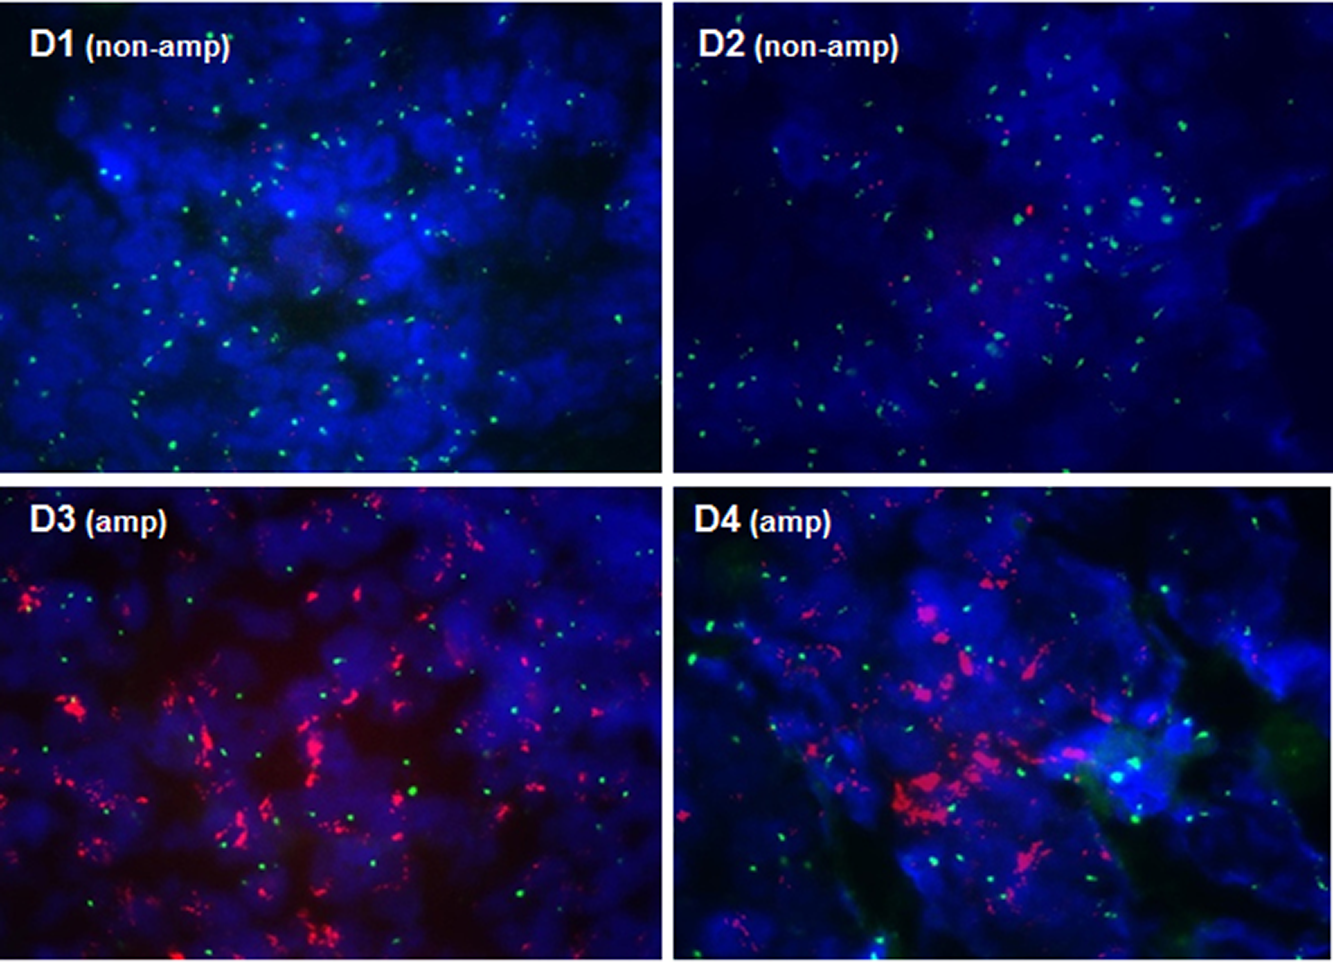
\includegraphics[width=0.8\textwidth]{methodology/images/fish-picture}}
\caption{FISH analysis of HER2 gene expression in samples of breast tumour. The probe mix consists of a mixture of Texas Red-labelled DNA probe against HER2 gene (which is located on chromosome 17) and a fluorescein (green)-labelled probe targeted at the centromeric region of chromosome 17. The upper panels (D1 and D2) show normal expression - 2 green and 2 red signals per cell. The lower panels (D3 and D4) show HER2 amplification whereby there is a clear increase in the red signal. [source: https://www.bioivt.com/fluorescent-in-situ-hybridization-fish/]}
\label{fig:fish-picture}
\end{figure}

Molecular diagnosis is the most recent approach in pathology. It mainly aims to support pathologists in the diagnosis of neoplastic diseases through the employment of molecular biology and cytogenetics techniques and it enables the deep understanding and monitoring of patients' profiles, as well as as defining the prognosis and ad-hoc therapies. All together, it allows the development of an increasingly personalised medicine, also in terms of research (e.g. understanding of pathological mechanisms and thus the possibilities of intervention).
However, it is still limited in its capabilities by the presence of a dishomogeneous information pool, especially in terms of knowledge extraction; a non-uniform data set entails, for the pathologist, an increased cognitive complexity because of having to manage a high number of variables and heterogeneous meaning behind the data; these consequently force to resort to problem decomposition and reduction.

In addition to its clinical support activities, the ICP also carries out scientific research aimed at better understanding certain types of cancers at translational level i.e., at the level of protein synthesis.
In the last ten years, the ICP has published more than 200 peer-reviewed papers and more than 100 works in non-peer reviewed journals and is active at a national and international level.

\subsection{Motivation} \label{subsec:motivation}
The Istituto Cantonale di Patologia already had a collaboration in place with the Dalle Molle Institute for Artificial Intelligence (IDSIA)\footnote{\url{http://www.idsia.ch}} to investigate a series of specific issues, whose details are outside of the scope of this thesis.
The prospect of the work to be carried out in this thesis was deemed of interest because it extended beyond the existing collaboration.
The institute had originally expressed interest in bringing machine learning into their workflow in order to both augment its profiling capabilities for patients and to be able to extract new knowledge from their existing data; this was paired with an attention for more experimental research directions, as the facilitation of human-machine interaction.

Given that the theoretical work carried out in this thesis is, at its core, an investigation into the explainability of Bayesian Networks, collaboration with the Institute provided the precious opportunity to implement a proof of concept system (described in Chapter \ref{chap:methodology} and \ref{chap:results}) based on a real medical data set and, most importantly, opened an opportunity for an \textit{application-grounded evaluation} of it (see Section \ref{sec:evaluation-of-explainability}).

The first contact with the ICP was in January 2019, during a meeting with Vittoria Martin (PhD), molecular cytogenetist, and Luca Mazzucchelli (Dr. Med.), director of the institute.
Since then, the clinicians and researchers of the ICP have been able to validate, from an Explainable AI and clinical relevance point of view, the model software that has been developed.
That is to say, they have validated, to an extent that will be made clear in Chapter \ref{chap:results}, the developed software both in its adherence to established medical literature and in its capacity to support clinical decision making and to surface clarifying explanations of the data set.
This is a great opportunity because the lack of real-world validation of ML systems with real domain experts is one of the prime gaps in the existing xAI literature (as discussed in depth in Chapter \ref{chap:literature-review}).

An example application for a clinician of the ICP, would be ability to \enquote{fill in the blanks} of a patient's profile, as it is not uncommon, for a variety of reasons, to have missing data.
This may be because of degraded or insufficient tissue samples or because some test may not yet be part of the standard diagnostic procedure, even though their importance may already be suggested by clinical research.
In other cases, patients may be missing a result because the specific test had not yet been invented, for example FISH was not available prior to 2010, so an a posteriori inference could be made possible.
Another crucial use may be in understanding and quantifying in an efficacious manner the relationship between clinical variables.
It is not uncommon for some variables to have been observed but for their clinical relevance not to have yet been determined; learning their relationship with other variables could potentially not only help in defining their importance in tracing new patient profiles in terms of diagnostic, prognosis and support in decision making but also in placing them in terms of pathological mechanisms.
These are all examples highlighting the importance of the \textit{inference} capabilities of machine learning and \textit{uncertain reasoning} techniques, but the current work aims to principally address the interfacing of the human user with the software while carrying out these queries.
It is also hoped that facilitating the process of knowledge-extraction may lead towards the confirmation of current scientific theories or may be the first step towards the formulation of novel ones.

\subsection{Provided Data Set}
The provided data set was created by \textit{Registro Tumori Ticino}\footnote{\url{https://www4.ti.ch/dss/dsp/icp/registro-cantonale-dei-tumori/home/}} (Locarno, Ticino) in order to highlight possible new relations between clinical, histopathological and molecular features, as well as to potentially discover novel biomarkers involved in the progression of the disease.
It consists of the histopathological records, over 38 variables of interest, of 3218 breast cancer patients who have been diagnosed between the years 2005 and 2014 within the Ticino canton of Switzerland.
The data set had already been pre-processed by collaborators of IDSIA under supervision of the ICP, with 13 of the variables being dropped because not relevant.
In particular, all variables relating to patients post-treatment were discarded as well as those recording the diagnosis date.
The data set was also anonymised, for obvious privacy issues.
Some of the variables were initially numerical (for example \enquote{FISH}) but all were converted to categorical.

In Table \ref{tab:datasetvariables} is a description of the remaining variables, together with their clinical meaning.
The distribution of the densities of the data set variables is shown in Table \ref{tab:datasetdistribution}.
The indications from Dr. Martin on how to further preprocess the data are shown in Table \ref{tab:datasetpreprocess}.
Note that some variable names were simplified and that the conversion to coarser categories should aid in boosting the explainability of the data set by reducing the number of possible values of each variable.

\begin{table*}[htbp]
\centering
\caption{Data set variables}
\begin{tabularx}{\textwidth}{@{} l Y @{}}
\toprule 
\textbf{Variable} & Clinical meaning \\
\midrule 
\textbf{Codice globale} & Unique patient identifier \\
\textbf{mut17q21} & Mutation of chromosome 17 \\
\textbf{loss 17} & Loss of chromosome 17 \\
\textbf{et\`a arrotondata} & The age of the patient at diagnosis \\
\textbf{Lateralit\`a} & The affected breast \\
\textbf{Situ SUBGROUP MZ} & The primary site code of the tumour \\
\textbf{Morfologia SUBGROUP MZ} & The morphology classification of the tumour \\
\textbf{pT SUBGROUP MZ} & Primary tumour dimensions in the TNM classification for breast cancer \\
\textbf{pN SUBGROUP MZ} & Pathologic nodes involvement in the TNM classification for breast cancer \\
\textbf{M 8.2.96} & Distant metastasis in the TNM classification for breast cancer \\
\textbf{Differenziazione} & Tumour grade \\
\textbf{Recettori estrogeni percento 1.1.2003} & Expression of estrogen receptors \\
\textbf{Recettori progestinici percento 1.1.2003} & Expression of progestin receptors \\
\textbf{c erbB 2  cod percento 1.1.2003} & ErbB2 marker expression \\
\textbf{Ki67 cod percento} & Tumoural proliferation index \\
\textbf{FISHRatio} & FISH analysis result \\
\bottomrule
\end{tabularx}
\label{tab:datasetvariables}
\end{table*}

\begin{table*}[htbp]
\centering
\caption{Data set distribution before pre-processing}
\begin{tabularx}{0.7\textwidth}{lXX}
\toprule 
\textbf{Variable} & Cardinality & Distribution \\
\midrule 
\textbf{mut17q21} & 2 &  
\includegraphics[width=0.2\textwidth, height=10mm]{methodology/images/mut17q21}\\
\textbf{loss 17} & 3 &  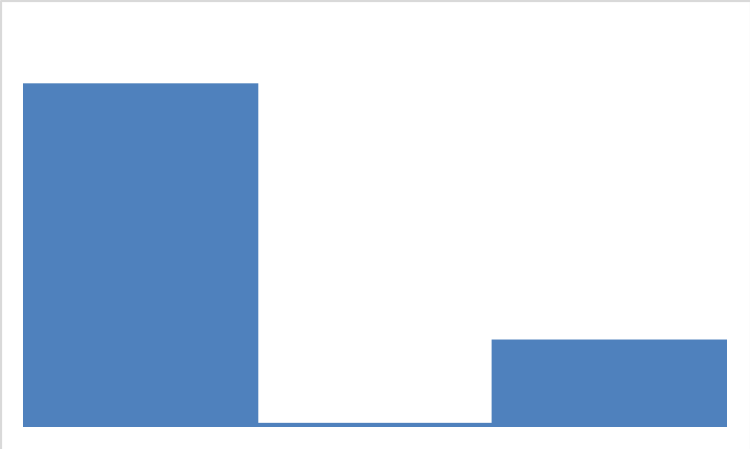
\includegraphics[width=0.2\textwidth, height=10mm]{methodology/images/loss_17}\\
\textbf{eta arrotondata} & 74 &  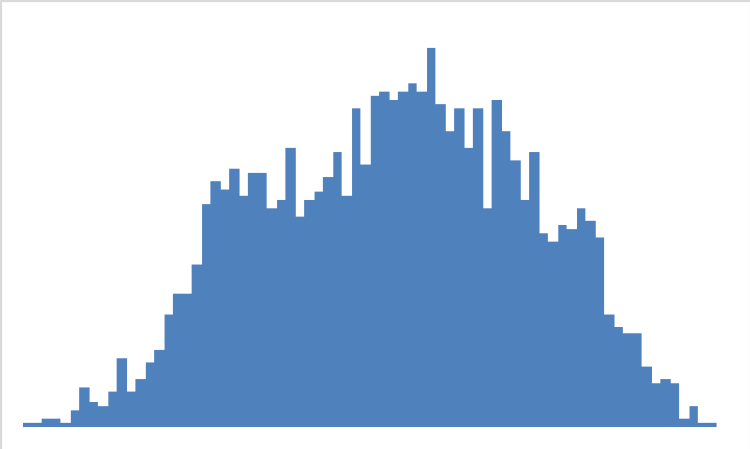
\includegraphics[width=0.2\textwidth, height=10mm]{methodology/images/eta_arrotondata}\\
\textbf{lateralit\`a} & 3 & 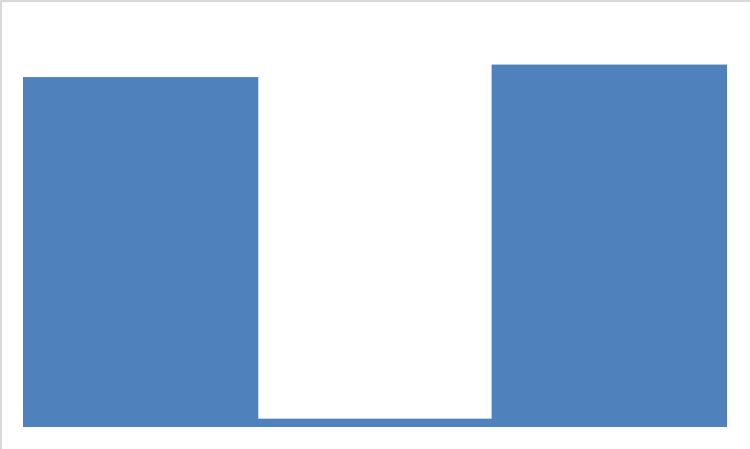
\includegraphics[width=0.2\textwidth, height=10mm]{methodology/images/lateralita} \\
\textbf{situ} & 5 & 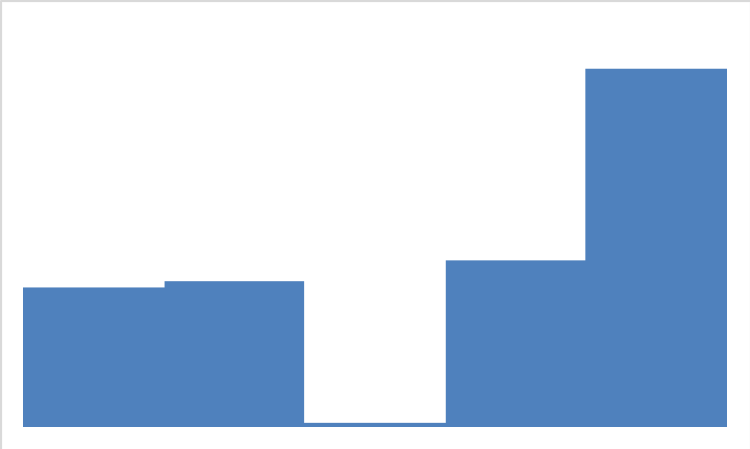
\includegraphics[width=0.2\textwidth, height=10mm]{methodology/images/situ} \\
\textbf{morfologia} & 5 & 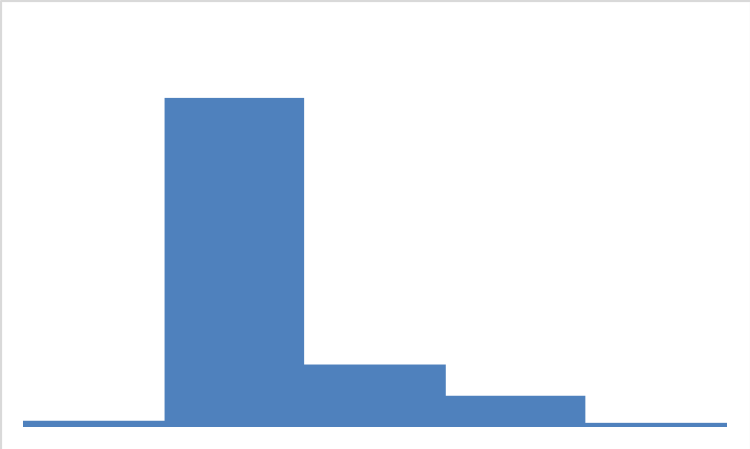
\includegraphics[width=0.2\textwidth, height=10mm]{methodology/images/morfologia} \\
\textbf{pT} & 23 & 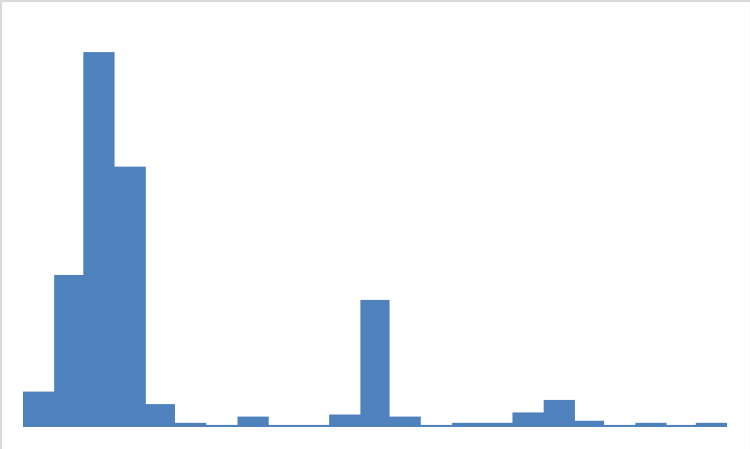
\includegraphics[width=0.2\textwidth, height=10mm]{methodology/images/pt} \\
\textbf{pN} & 6 & 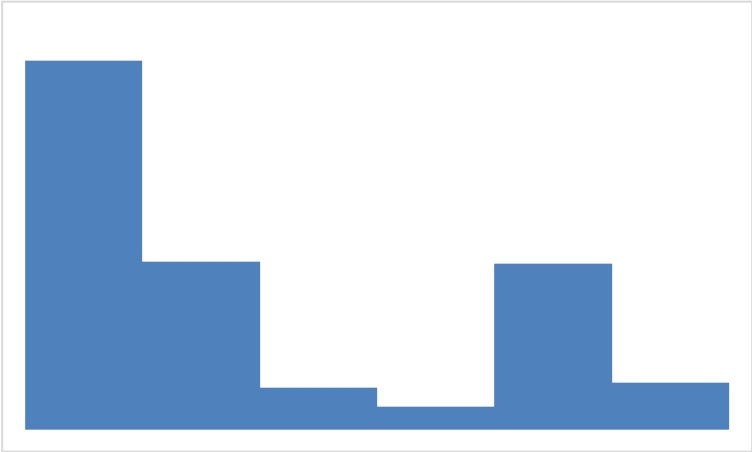
\includegraphics[width=0.2\textwidth, height=10mm]{methodology/images/pn} \\
\textbf{M} & 3 & 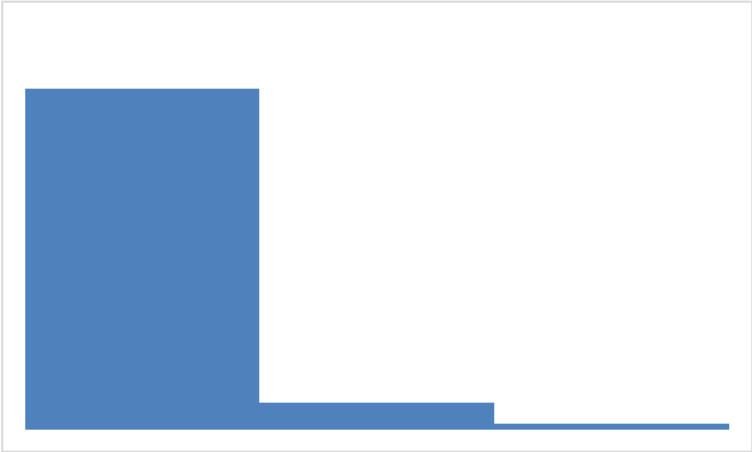
\includegraphics[width=0.2\textwidth, height=10mm]{methodology/images/m} \\
\textbf{differenziazione} & 5 & 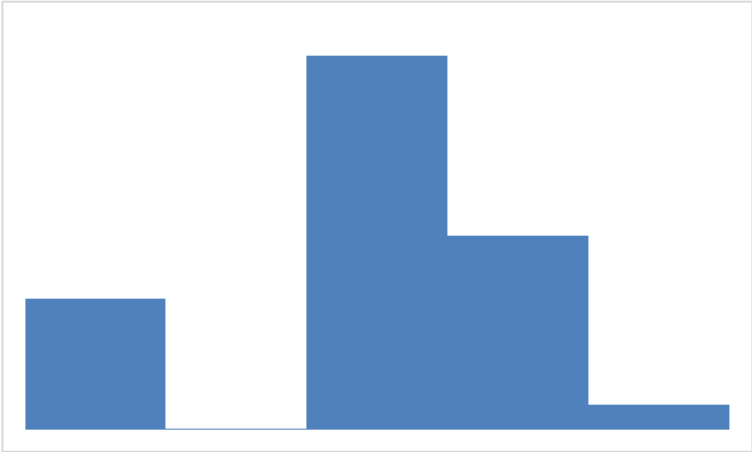
\includegraphics[width=0.2\textwidth, height=10mm]{methodology/images/differenziazione}  \\
\textbf{recettori estrogeni} & 40 & 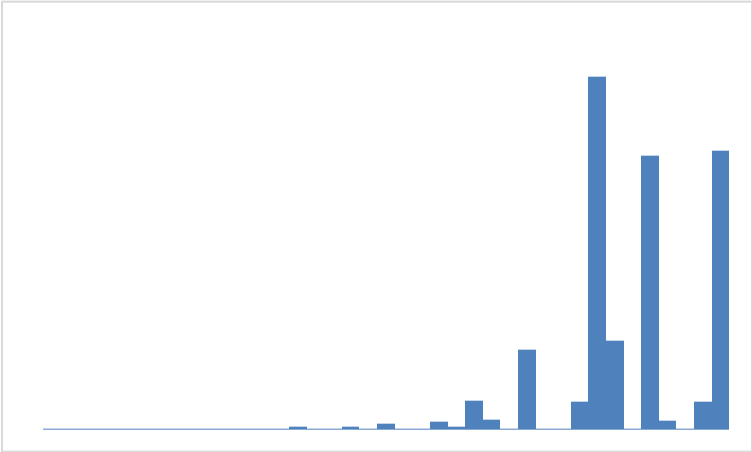
\includegraphics[width=0.2\textwidth, height=10mm]{methodology/images/recettori_estrogeni} \\
\textbf{recettori progestinici} & 40 & 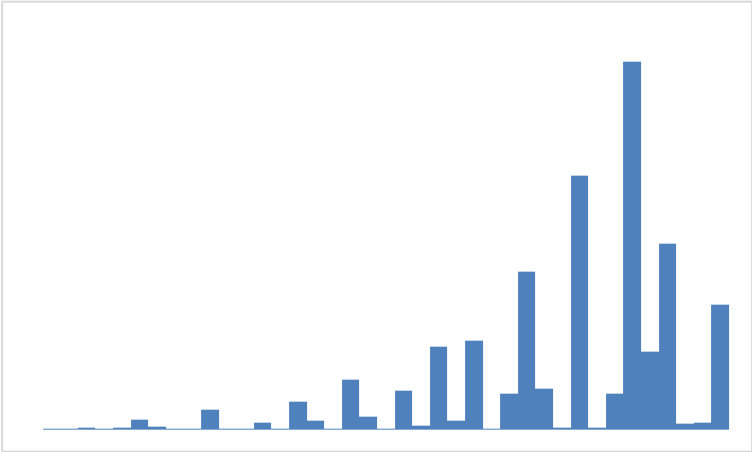
\includegraphics[width=0.2\textwidth, height=10mm]{methodology/images/recettori_progestinici}\\
\textbf{c erbB 2} & 4 & 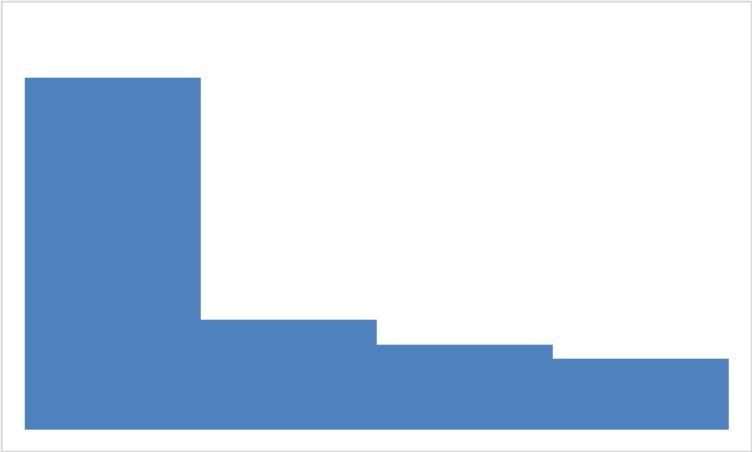
\includegraphics[width=0.2\textwidth, height=10mm]{methodology/images/c_erb_2}\\
\textbf{Ki67} & 52 & 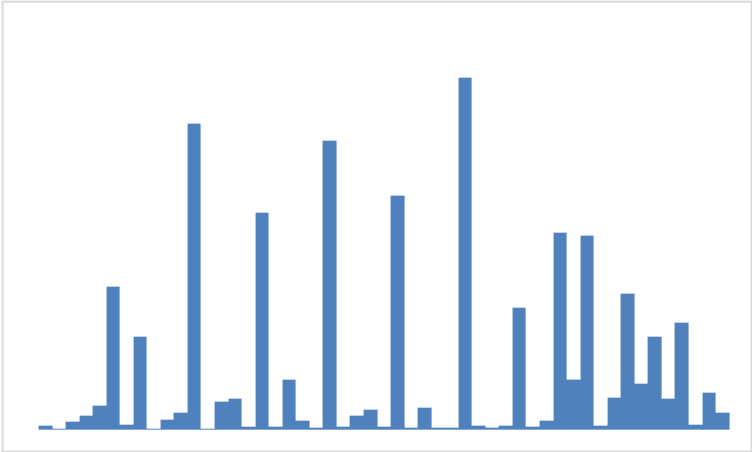
\includegraphics[width=0.2\textwidth, height=10mm]{methodology/images/ki67}\\
\textbf{FISHRation} & 5 &  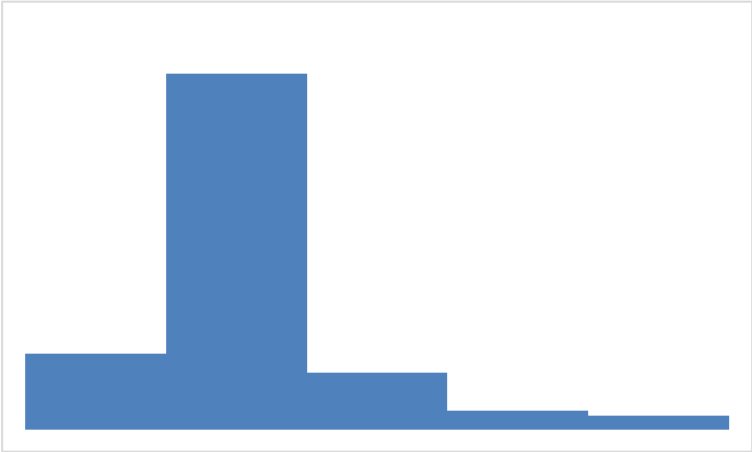
\includegraphics[width=0.2\textwidth, height=10mm]{methodology/images/fish}\\
\bottomrule
\end{tabularx}
\label{tab:datasetdistribution}
\end{table*}

\begin{table*}[htbp]
\centering
\caption{Data set preprocessing steps}
\begin{tabularx}{\textwidth}{@{} l Y @{}}
\toprule 
\textbf{Variable} & Action \\
\midrule 
\textbf{Codice globale} & Remove variable \\
\textbf{mut17q21} & Remove variable \\
\textbf{loss 17} & Remove variable \\
\textbf{eta arrotondata} & Bin into \enquote{$< 40$}, \enquote{$40-50$}, \enquote{$\geq 50$} \\
\textbf{lateralita} & Remove blanks and \enquote{sconosciuta} \\
\textbf{situ} & Remove blanks \\ \addlinespace
\textbf{morfologia} & Remove blanks and \enquote{unuseful} if performance on classification is subpar \\ \addlinespace
\textbf{pT} & Remove blanks and \enquote{unuseful}  \\
\textbf{pN} & Remove blanks and bin into \enquote{0} and \enquote{$\neq0$}\\
\textbf{M} & Remove blanks \\ 
\textbf{differenziazione} & Remove blanks and \enquote{Sconosciuto o non applicabile} \\ \addlinespace
\textbf{recettori estrogeni} & Remove blanks and bin into \enquote{negativo} if $\leq 10$,
		\enquote{debolmente positivo} if $\leq 50$, 
		\enquote{fortemente positivo} if $> 50$ \\ \addlinespace
\textbf{recettori progestinici} & Remove blanks and bin into \enquote{negativo} if $\leq 10$, 
		\enquote{debolmente positivo} if $\leq 50$, 
		\enquote{fortemente positivo} if $> 50$ \\ \addlinespace
\textbf{c erbB 2} & Remove blanks \\ 
\textbf{ki67} & Remove blanks and bin into \enquote{<14}, 
		\enquote{14-20}, \enquote{20-30}, \enquote{>30} \\ 
\textbf{FISH} & Remove variable \\
\bottomrule
\end{tabularx}
\label{tab:datasetpreprocess}
\end{table*}


% !TEX root = thesis-thomas-tiotto.tex

\section{Methods}
\subsection{Libraries}
\subsubsection{pomegranate}
Pomegranate (\cite{pomegranate}) is an open-source probabilistic models package for python.
Its core philosophy is that every probabilistic model, from Hidden Markov to Bayesian Network, can be seen as a probability distribution and, as such, can be flexibly composed into hierarchical mixture models (\cite{Schreiber2017}).
The package implements:
\begin{itemize}
	\item Probability Distributions
	\item General Mixture Models
	\item Hidden Markov Models
	\item Bayes Classifiers and Na{\"i}ve Bayes
	\item Markov Chains
	\item \textbf{Bayesian Networks}
	\item Factor Graphs
\end{itemize} 

This package was chosen among others for its good implementation of Bayesian Networks, its clear API and its performance.
The package is written in cython and natively supports multi-core parallelism and out-of-core learning.
Network structure learning from data, described in \ref{subsec:bnstructurelearning}, appears to be particularly efficient, thanks to the implementation of prior knowledge into the graph selection process as described by \cite{schreiber_noble_2017}.
The claim of this novel selection process is that it possesses the speed of a heuristic approach while yielding a far better quality estimate.

pomegranate currently only supports Discrete Bayesian Networks so the random variable of each node must have a categorical distribution.

\textit{Structure learning} from data is achieved using the \texttt{from\_samples} method of the \texttt{BayesianNetwork} class, with the default algorithm being the novel one described by \cite{schreiber_noble_2017}.
The \textit{probability} of a sample is calculated using the \texttt{probability} function of an object of \texttt{BayesianNetwork} type; the \texttt{predict\_proba} function is used to return the probability of each variable in the model given some evidence.
\textit{Predictions} (described in detail in Sec. \ref{subsec:bnupdating}) are run by passing to the \texttt{predict} function of an object a matrix with \texttt{None} as placeholders for missing values .
\textit{Fitting} is done thought the \texttt{fit} function that uses MLE estimates to update each node's distribution in the model based on the input data.

A \texttt{BayesianNetwork} object can also be displayed graphically by calling its \texttt{plot} function.
The output is a DOT file that is generated using the PyGraphviz package (\cite{pygraphviz}), that is a python interface to the famous Graphviz (\cite{graphviz}) graph visualisation software.
An example of such an output is shown in Fig. \ref{fig:pomegranate_graph_example}.

\begin{figure}[htbp]
\centerline{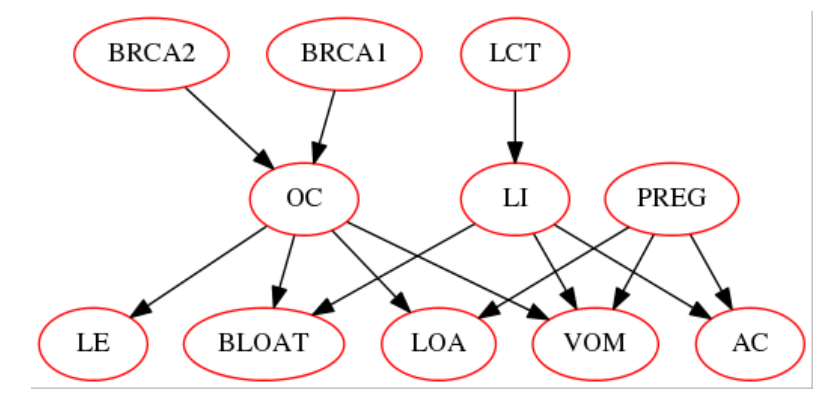
\includegraphics[width=\columnwidth]{methodology/images/pomegranate_example}}
\caption{Example output of \texttt{plot} (\cite{pomegranatetutorial}) }
\label{fig:pomegranate_graph_example}
\end{figure}

\subsubsection{pandas}
\subsubsection{scikit-learn}
\subsubsection{numpy}
\subsubsection{networkx}
\subsection{Algorithms}
\subsubsection{d-separation}
\subsubsection{MPE}
\section{Novel contributions}\label{sec:novel-contributions}
 \todo{tengo qui o sposto nel cap 4?}

\subsection{Theory} \label{subsec:theory}
\todo{la discussione con l'esperto ci da' belief revision dei dati}
\todo{counterfactual explanations}
\todo{magari togliere theory e mettere tutto assieme}

\subsubsection{Selection based on entropy}
\todo{utilizzo entropia}

\subsection{Algorithms}
An important part of my work was developing the algorithms needed to adapt the ideas presented in the paper \enquote{Explaining the Most Probable Explanation} by \cite{Butz2018} and \enquote{A Progressive Explanation of Inference in \enquote{Hybrid} Bayesian} by \cite{Kyrimi2016}.
From the former, the construction of the probability tree through a constructive dialogue with the domain expert, the building of counterfactual explanation branches, the automatic generation of the most probable probability tree from initial evidence.
From the latter, the generation of an \enquote{Inverse explanation}.
Finally, a simple procedure to output a natural language explanation was developed.

\subsubsection{\enquote{Pseudo-MPE}} \label{subsubsec:pseudo-mpe}
\todo{dove critico il fatto che non calcolano veramente l'MPE come dicevano? qui o in cap.4 on cap.2?}
The so-called \enquote{Pseudo-MPE} algorithm is inherently wrapped up with the concept of \textit{dialogue} and is central to the explanatory powers of the system being developed in this thesis.
The algorithm was developed as a way of implementing the \enquote{MPE branch} of the \enquote{Argumentative Probability Tree} hypothesised by \cite{Butz2018}.
It was termed \enquote{Pseudo-MPE} because there are no guarantees of it returning the MPE solution (see Subsec. \ref{subsec:bnupdating}), as noted by \cite{koller2007introduction} in their definition of the MAP problem.

At a lower level of detail, the algorithm may be broken into:
\begin{itemize}
	\item a dialogical part, that interfaces with the expert user through the use of natural language, menus and visualisations
	\item the part responsible for constructing the \enquote{MPE branch}
\end{itemize}
The former process was informed and shaped by the results obtained by the methods described in Subsec. \ref{subsec:explainability-validation} and, as such, presented substantial elements of novelty.

The latter process is, at its core, a greedy procedure that aims at selecting the \enquote{best} next $(state, value)$ tuple at each step, based on some measure of optimality and on the variables already in the evidence set.
In the actual implemented system the two parts are intertwined, given their close inter-dependence.

The \texttt{dialogue} procedure starts by asking the user to select a subset of variables and their relative values to add as initial evidence.
This initial evidence is used to radicate the MPE Branch.
It should be noted than in the description given by \cite{Butz2018}, the Argumentative Probability Tree is a real tree as each node is guaranteed to have at most one parent.
My application, on the other hand, constructs an \textit{Argumentative Probability Polytree} (see Subsec. \ref{subsec:polytrees}) because, as will better be described in Chap. \ref{chap:results}, it was seen early on that the users much preferred to be able to start from a set of initial evidences and not be limited to a single one.
The algorithm then proceeds to call the \texttt{next\_most\_probable\_states} subroutine that is tasked with returning an ordered list of $(state,value)$ pairs.
It does this by calculating the posterior distribution given evidence of all the states not already in the evidence, then calculating the efficiency (see \ref{subsec:normalised-entropy}) and the maximally probable symbol of each state's distribution and finally returning the $(state,value)$ tuples ordered according to their normalised entropy (most efficient/least entropic at the head).
The $(state,value)$ pair at the head of the list is proposed to the user who has the faculty to accept the system's evaluation or refuse it.
If the user accepts, the state is added to the evidence set and to the MPE Branch under construction.
Thus, the evidence set's cardinality increases by one each time a user accepts a proposal.
The updated evidence will be used to calculate the new list of $(state,value)$ pairs at the following round.
If the expert chooses to refuse, then she is iteratively presented with the remaining $(state,value)$ items, in order of decreasing efficiency. 
Once she accepts one of the explanations given by the system, the \texttt{generate\_alternative\_branch} subroutine is called to automatically generate a maximally probable MPE Branch, radicated in the newest $(state,value)$ node of the MPE Branch.
The proposal loop for alternative states runs until there are increasingly less probable elements in the list and exits with a partial solution if the user refuses all of them at a given step.
Thus, the Pseudo-MPE solution is constructed only if the user runs through all variables proposed, accepting each one at least once.

Three slightly different operational modes of the algorithm were implemented.
This was done for research purposes, in order to understand which of the three, if any or if a combination of their distinctive features, the expert users would find the most useful from a usability, comprensibility and explainability standpoint:
\begin{itemize}
  \item exhaustive: In the basic dialogue type, the set of variables under consideration monotonically decreases by one every time the user accepts one of the system's proposals and the dialogue terminates only when the user has accepted all variables at least once or refused all proposals at a given step.
	In the first case the user will have the Pseudo-MPE solution while in the second she will be left with a partial assignment to some of the variables not present in the initial evidence.
	The pseudocode is shown in Alg. \ref{alg:pseudo-mpe-exhaustive}.
  \item d-separated: In the second variant, the set of variables under considered at each step is dynamic and depends on the separation properties of the underlying Bayesian Network's DAG and the evidence set constructed by the user's choices.
  	Differently from the first type of dialogue, an additional \texttt{evidence\_d\_separation} subroutine is called before \texttt{next\_most\_probable\_states} to calculate the set of variables that are d-separated from the evidence set, up to that step of the dialogue.
  	\texttt{next\_most\_probable\_states} is then executed but the variables that the previous function found to be separated from the evidence, are removed from the returned list.
  	This way, variables that can have no effect given the current evidence are not proposed.
  	As the d-separation operation is not monotonic, adding new nodes to the evidence set can both increment or diminish the number of nodes that will be proposed at each step.
  	The user is shown an updated view of the independencies of the graph at each step; an example of such an output is shown in Fig. \ref{fig:pseudo-mpe-independencies_1} and \ref{fig:pseudo-mpe-independencies_2}.
  	The pseudocode is shown in Alg. \ref{alg:pseudo-mpe-independencies}.
  \item thresholded: The final variant of the algorithm prunes the set of variables using a different strategy from the previously presented one.
  	In this case, the $(state,value)$ pairs in the list returned by \texttt{next\_most\_probable\_states} are dropped automatically based on their probability.
  	Pairs whose probability is below a user-defined threshold or are \enquote{worse than random} (for ex. a $(state,value)$ tuple will be discarded if $state$ is binary and the probability of $value$ is lower than $0.5$) are removed and not proposed to the user. 
  	This thresholding strategy based on the probability of the tuples is paired with one where there is a user-defined threshold on the number of times that the expert can refuse a particular $(state,value)$. 
  	In the general dialogue, tuples can be proposed multiple times, with an ever lower probability, if the user has previously refused them; in the thresholded scheme a $(state,value)$ pair can only be proposed a maximum number of times before being permanently discarded.
\end{itemize}

The underlying Bayesian Network that represents the data set is learned and queried through the  \texttt{pomegranate} (see Subsec. \ref{subsec:libraries}), API but the great majority of all the code is completely custom-written.
This was necessary because \texttt{pomegranate}, while having a powerful backend, was found to be severely lacking in the breadth and flexibility of its API.
Many basic operations, such as the calculation of a joint distribution, were not available so the only way was to implement lower-level workarounds while still using \texttt{pomegranate} for the most basic operations, as the calculation of a posterior distribution.
In particular, \texttt{dialogue} is implemented with the only direct calls to the API being when learning the network and when calling \texttt{predict\_proba}, that queries the \texttt{BayesianNetwork} object to calculate the posterior distribution of the states given the current evidence.
D-separation, in the second variant of the algorithm, is calculated via the \texttt{evidence\_d\_separation} procedure that implements the pseudocode presented in Alg. \ref{alg:d-separation}.

\begin{algorithm}[htp!]
	\caption{Exhaustive pseudo-MPE algorithm}
	\label{alg:pseudo-mpe-exhaustive}
	\begin{algorithmic}[1]
		\State $evidence = $ user selected $(state,value)$ tuples
		\State $MPE\_polytree = $ MPE Polytree rooted in $evidence$
		\While{True} 
			\State $mpe\_states$ = \texttt{next\_most\_probable\_states($evidence$)}
			\If{$mpe\_states$ is not empty}
				\State $next\_state$ = head of $mpe\_states$ 
				\State propose $next\_state$ to user \Comment{the least entropic state}
				\If{the user refuses $next\_state$}
					\For{$alternative\_state$ in $mpe\_states \smallsetminus next\_state$}
						\State propose $alternative\_state$ to user \Comment{the next least entropic states}
						\If{the user accepts $alternative\_state$}
							\State call \texttt{generate\_alternative\_branch()} on $MPE\_polytree$ 
							\State add $alternative\_state$ to $MPE\_polytree$
							\State $evidence = evidence \cup alternative\_state$
						\Else
							\State continue
						\EndIf
					\EndFor
				\Else
					\State add $next\_state$ to $MPE\_polytree$
					\State $evidence = evidence \cup next\_state$
				\EndIf
			\Else 
				\State return
			\EndIf
		\EndWhile
	\end{algorithmic}
\end{algorithm} 

\begin{algorithm}[htp!]
	\caption{Independencies pseudo-MPE algorithm}
	\label{alg:pseudo-mpe-independencies}
	\begin{algorithmic}[1]
		\State $evidence = $ user selected $(state,value)$ tuples
		\State $MPE\_polytree = $ MPE Polytree rooted in $evidence$
		\While{True} 
			\State $separated = $ \texttt{evidence\_d\_separation($evidence$)} \Comment{based on evidence of previous step}
			\State $mpe\_states$ = \texttt{next\_most\_probable\_states($evidence$)}
			\State $mpe\_states = mpe\_states \smallsetminus separated$ 
			\If{$mpe\_states$ is not empty}
				\State $next\_state$ = head of $mpe\_states$ 
				\State propose $next\_state$ to user \Comment{the least entropic state}
				\If{the user refuses $next\_state$}
					\For{$alternative\_state$ in $mpe\_states \smallsetminus next\_state$}
						\State propose $alternative\_state$ to user \Comment{the next least entropic states}
						\If{the user accepts $alternative\_state$}
							\State call \texttt{generate\_alternative\_branch()} on $MPE\_polytree$ 
							\State add $alternative\_state$ to $MPE\_polytree$
							\State $evidence = evidence \cup alternative\_state$
						\Else
							\State continue \Comment{go to next proposal}
						\EndIf
					\EndFor
				\Else
					\State add $next\_state$ to $MPE\_polytree$
					\State $evidence = evidence \cup next\_state$
				\EndIf
			\Else 
				\State return 
			\EndIf
		\EndWhile
	\end{algorithmic}
\end{algorithm} 

\begin{figure}[htbp]
\centerline{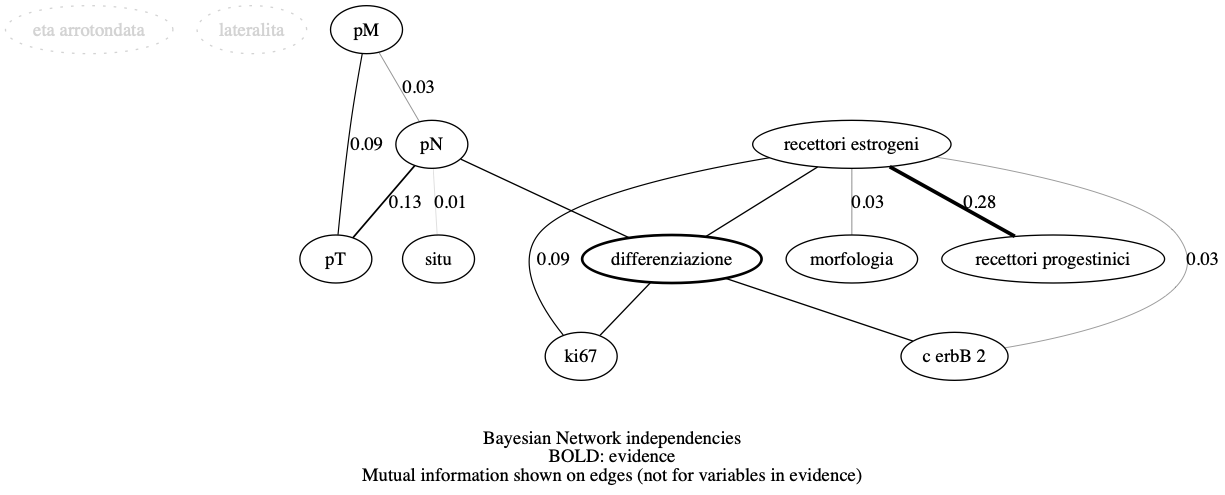
\includegraphics[width=\columnwidth]{methodology/images/example-d-separation-mpe_1}}
\caption{Example output during the first round of the d-separation-aware variant of \texttt{dialogue}.
	The variable \enquote{mut17q21} is the initial evidence.}
\label{fig:pseudo-mpe-independencies_1}
\end{figure}

\begin{figure}[htbp]
\centerline{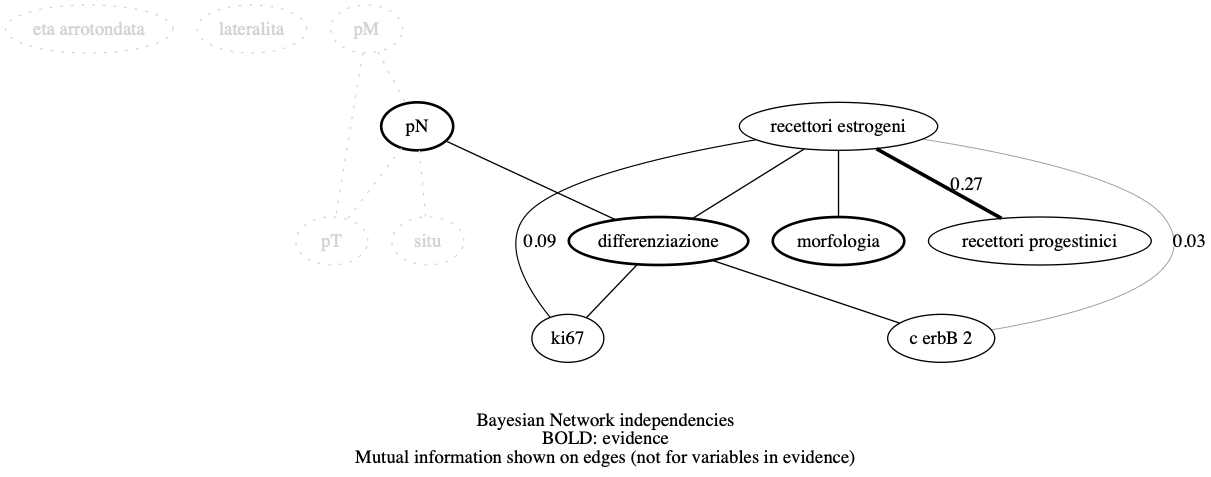
\includegraphics[width=\columnwidth]{methodology/images/example-d-separation-mpe_2}}
\caption{Example output during the second round of the d-separation-aware variant of \texttt{dialogue}.
	\enquote{morfologia} is added to the evidence set and this makes a large part of the network redundant.}
\label{fig:pseudo-mpe-independencies_2}
\end{figure}

\begin{algorithm}[htp!]
	\caption{Thresholded pseudo-MPE algorithm}
	\label{alg:pseudo-mpe-thresholded}
	\begin{algorithmic}[1]
		\State user selected $refuse\_bound$
		\State $refuse\_thresholds = \emptyset$
		\State $lower\_thresholds = \emptyset$
		\For{$v \in V$}
			\For{value $k$ of $v$}
				\State element $[v,k]=0$ in $refuse\_thresholds$
			\EndFor
			\State element $[v]=1 / |v|$ in $lower\_thresholds$ \Comment{refuse worse than random pairs}
		\EndFor
		\State $evidence = $ user selected $(state,value)$ tuples
		\State $MPE\_polytree = $ MPE Polytree rooted in $evidence$
		\State $mpe\_states$ = \texttt{next\_most\_probable\_states($evidence$)}
		\While{True} 
			\For{$s \in mpe\_states$}
				\If{probability of $s < lower\_thresholds[s] \wedge refuse\_thresholds[s] > refuse\_bound$}
					\State remove $s$ from $mpe\_states$ 
				\EndIf
			\EndFor		
			\If{$mpe\_states$ is not empty}
				\State $next\_state$ = head of $mpe\_states$ 
				\State propose $next\_state$ to user \Comment{the least entropic state}
				\If{the user refuses $next\_state$}
					\State increment $refuse\_thresholds[next\_state]$
					\For{$alternative\_state$ in $mpe\_states \smallsetminus next\_state$}
						\State propose $alternative\_state$ to user \Comment{the next least entropic states}
						\If{the user accepts $alternative\_state$}
							\State call \texttt{generate\_alternative\_branch()} on $MPE\_polytree$ 
							\State add $alternative\_state$ to $MPE\_polytree$
							\State $evidence = evidence \cup alternative\_state$
						\Else
							\State increment $refuse\_thresholds[alternative\_state]$
							\State continue
						\EndIf
					\EndFor
				\Else
					\State add $next\_state$ to $MPE\_polytree$
					\State $evidence = evidence \cup next\_state$
				\EndIf
			\Else 
				\State return
			\EndIf
		\EndWhile
	\end{algorithmic}
\end{algorithm} 

\subsubsection{Alternative Explanation Branches}
The function to generate alternative branches to the main MPE branch in the dialogue tree is called after the user refuses a $(state,value)$ in the dialogue and accepts one of the the alternatives.
The motivation is to present the user with a simple \enquote{what-if} analysis, replying to the question \enquote{Had I accepted the $(state,value)$ presented me by the system, what would have been the most probable configuration of the remaining $(state,value)$ pairs?}.
The question is answered by generating a maximally probable, alternative MPE sub-branch rooted in the last node in the main MPE branch that is under construction through the dialogue.

The alternative branch is generated by what is essentially an automated version of \texttt{dialogue} that always accepts the first suggestion returned by \texttt{next\_most\_probable\_states}.
Given that \texttt{dialogue} and \texttt{generate\_alternative\_branch} are essentially one and the same, the latter inherits the same pruning strategies as the former.
That is, \texttt{generate\_alternative\_branch} called during the exhaustive dialogue will generate a maximally likely assignment over all variables in $V \smallsetminus E$ while when invoked from one of the other two variant of the dialogue algorithm, it will apply their same pruning strategies.

The implementation of the MPE Polytree is based on the \texttt{NetworkX} python package (see Subsec. \ref{subsec:libraries}).
The creation of a chain of nodes is done by keeping a local pointer $alt\_node$ that refers to the last added node or set of nodes, if the node being added is the successor of multiple initial evidences. 

An example of the output shown to the user at each step of the dialogue is shown in Fig. \ref{fig:alternative-branch} while the pseudocode for the three variants are shown in Alg. \ref{alg:alternative-branch-echaustive}, \ref{alg:alternative-branch-independencies} and \ref{alg:alternative-branch-thresholded}.
Note that $alternative\_evidence$ is local to this algorithm and is separate from the $evidence$ used in the main \texttt{dialogue} procedure.

\begin{figure}[htbp]
\centerline{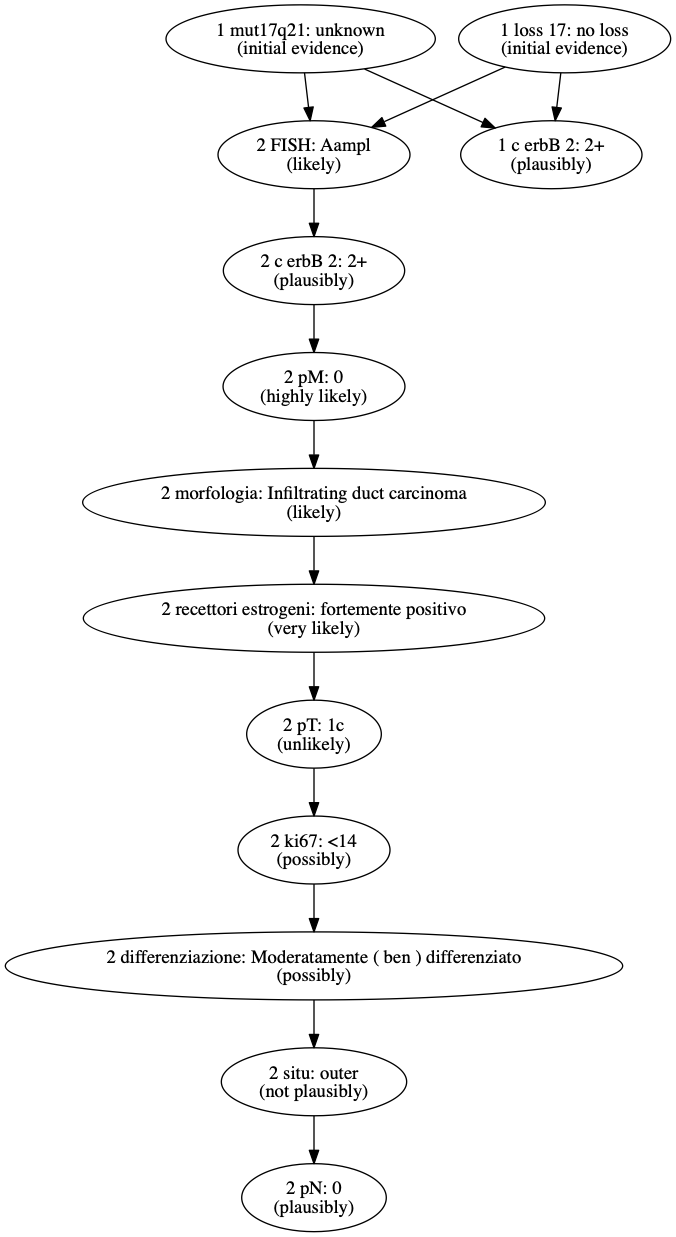
\includegraphics[scale=0.2]{methodology/images/alternative-explanation-tree-example}}
\caption{Example output during the d-separation-aware variant of \texttt{dialogue}.
	The tuple (\enquote{FISH},\enquote{Aampl}) was proposed but the expert refused it and accepted the alternative (\enquote{c erbB 2},\enquote{2+}).
	The main MPE Branch has ID 1 while the \enquote{what-if} one has ID 2.}
\label{fig:alternative-branch}
\end{figure}

\begin{algorithm}[htp!]
	\caption{Exhaustive alternative explanation branch algorithm}
	\label{alg:alternative-branch-echaustive}
	\begin{algorithmic}[1]
		\State $alternative\_evidence = evidence$ 
		\State $alt\_node = $ last node in the main MPE Polytree
		\State $branch\_id = branch\_id + 1$
		\While{True} 
			\State $mpe\_states$ = \texttt{next\_most\_probable\_states($alternative\_evidence$)}
			\If{$mpe\_states$ is empty}
				\State return
			\Else
				\State $next\_state$ = head of $mpe\_states$ 
				\State create $next\_state$ node, tag it with $branch\_id$ and make it son of $alt\_node$
				\State update $alt\_node$ node to be $next\_state$ node
				\State $alternative\_evidence = alternative\_evidence \cup next\_state$
			\EndIf
		\EndWhile
	\end{algorithmic}
\end{algorithm}

\begin{algorithm}[htp!]
	\caption{Independencies alternative explanation branch algorithm}
	\label{alg:alternative-branch-independencies}
	\begin{algorithmic}[1]
		\State $alternative\_evidence = evidence$ 
		\State $alt\_node = $ last node in the main MPE Polytree
		\State $branch\_id = branch\_id + 1$
		\While{True} 
			\State $separated = $ \texttt{evidence\_d\_separation($alternative\_evidence$)}
			\State $mpe\_states$ = \texttt{next\_most\_probable\_states($alternative\_evidence$)}
			\State $mpe\_states = mpe\_states \smallsetminus separated$ 
			\If{$mpe\_states$ is empty}
				\State return
			\Else
				\State $next\_state$ = head of $mpe\_states$ 
				\State create $next\_state$ node, tag it with $branch\_id$ and make it son of $alt\_node$
				\State update $alt\_node$ node to be $next\_state$ node
				\State $alternative\_evidence = alternative\_evidence \cup next\_state$
			\EndIf
		\EndWhile
	\end{algorithmic}
\end{algorithm} 

\begin{algorithm}[htp!]
	\caption{Thresholded alternative explanation branch algorithm}
	\label{alg:alternative-branch-thresholded}
	\begin{algorithmic}[1]
		\State $alternative\_evidence = evidence$ 
		\State $alt\_node = $ last node in the main MPE Polytree
		\State $branch\_id = branch\_id + 1$
		\While{True} 
			\For{$s \in mpe\_states$}
				\If{probability of $s < lower\_thresholds[s] \wedge refuse\_thresholds[s] > refuse\_bound$}
					\State remove $s$ from $mpe\_states$ 
				\EndIf
			\EndFor	
			\State $mpe\_states$ = \texttt{next\_most\_probable\_states($alternative\_evidence$)}
			\If{$mpe\_states$ is empty}
				\State return
			\Else
				\State $next\_state$ = head of $mpe\_states$ 
				\State create $next\_state$ node, tag it with $branch\_id$ and make it son of $alt\_node$
				\State update $alt\_node$ node to be $next\_state$ node
				\State $alternative\_evidence = alternative\_evidence \cup next\_state$
			\EndIf
		\EndWhile
	\end{algorithmic}
\end{algorithm} 

\todo{ancora da implementare true MPE}
\subsubsection{\enquote{Pseudo-MPE} from Random Evidence} \label{subsubsec: pseudo-mpe-random}
In order to compare the Pseudo-MPE output with the true MPE solution I implemented a simple algorithm that, starting from a random initial set of evidence, generates the relative pseudo-MPE and MPE solutions.
The random initial evidence set is constructed by randomly choosing a number in the interval $k = [ 1, |V| ]$, with $V$ the set of vertices in the BN, and then randomly selecting $k$ of the random variables in $V$ to yield the set of variables $E$.
The value of each variable is randomly chosen among the set of its values; as all variables are categorical, this can easily be done.

The implementation is based on the \texttt{NetworkX} python library (see Subsec. \ref{subsec:libraries}) package as what is being constructed is not a tree but a \textit{polytree} (see Subsec. \ref{subsec:polytrees}), as nodes may have multiple parents.
Note that $alternative\_evidence$ is considered separate from the main $evidence$ used in \texttt{dialogue}.

The pseudocode is shown in Alg. \ref{alg:pseudo-mpe-random-evidence} while an example output can be seen in Fig. \ref{fig:pseudo-mpe-random}.

\begin{algorithm}[htp!]
	\caption{Pseudo-MPE from random evidence algorithm}
	\label{alg:pseudo-mpe-random-evidence}
	\begin{algorithmic}[1]
		\State $evidence = \emptyset$
		\State generate random number $k \in [ 1, |V| ]$
		\State $S = $ choose $k$ variables from $V$
		\For{$s \in S$}
			\State choose random $v$ in the possible values of $e$ 
			\State $evidence = evidence \cup (s,v)$
		\EndFor
		\State $MPE\_polytree = $ MPE Polytree rooted in $evidence$
		\State $last\_node = evidence$
		\State $alternative\_evidence = evidence$ 
		\While{True} 
			\State $mpe\_states$ = \texttt{next\_most\_probable\_states($alternative\_evidence$)}
			\If{$mpe\_states$ is empty}
				\State return
			\Else
				\State $next\_state$ = head of $mpe\_states$ 
				\State create $next\_state$ node and make it son of $last\_node$
				\State update $alt\_node$ node to be $next\_state$ node
				\State $alternative\_evidence = alternative\_evidence \cup next\_state$
			\EndIf
		\EndWhile
	\end{algorithmic}
\end{algorithm}

\begin{figure}[htbp]
\centerline{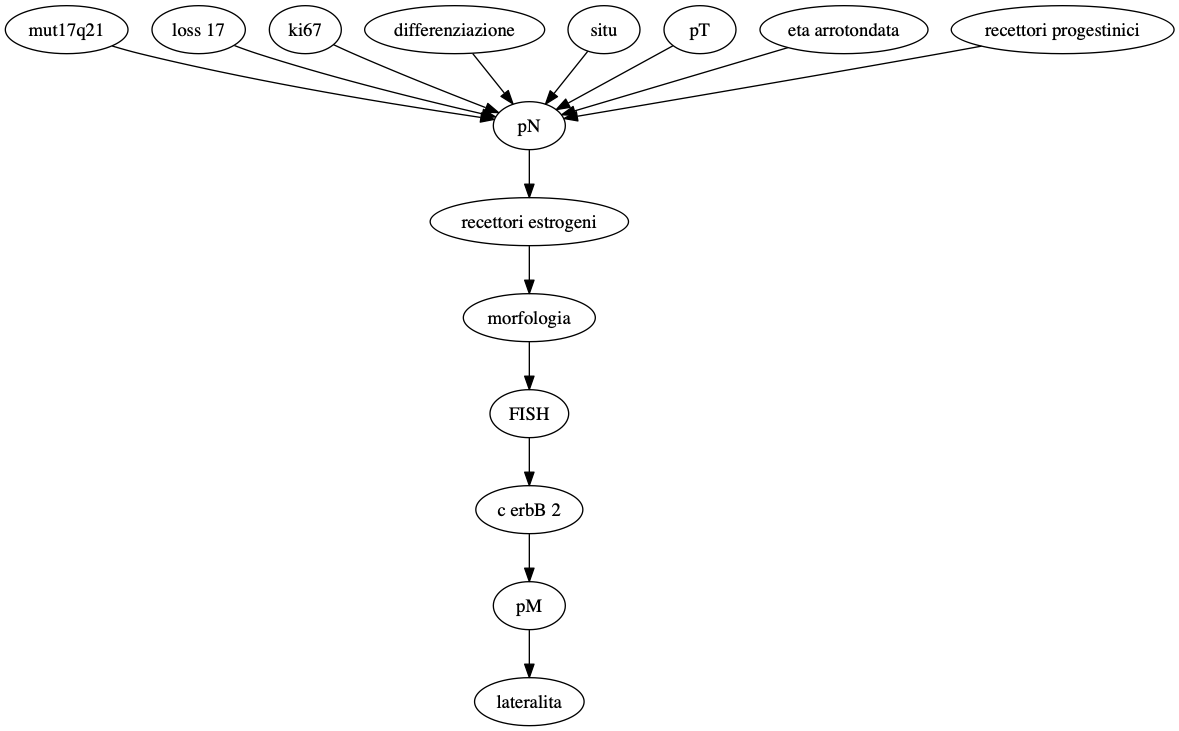
\includegraphics[width=\columnwidth]{methodology/images/pseudo-mpe-random-example}}
\caption{Example output of the Pseudo-MPE from random evidence algorithm.}
\label{fig:pseudo-mpe-random}
\end{figure}

\subsubsection{Inverse Explanation}
\todo{da fare e trovare nome migliore}

\subsubsection{Natural Language Explanation}
\todo{da fare e magari pensare anche a visual explanations?}
The probability of each proposed tuple is quantified in natural language based on the probability of the most probable value within the variable.
These are shown in Tab. \ref{tab:naturallanguageprobabilities}.

\begin{table*}[htbp]
\caption{Probability quantifiers in natural language}
\begin{tabularx}{\textwidth}{@{} X X @{}}
\toprule 
Probability range & Natural language quantifier \\
\midrule 
(0, 0.2) &  "highly unlikely" \\
(0.2, 0.3) & "very unlikely" \\
(0.3, 0.4) & "unlikely" \\
(0.4, 0.5) & "not plausibly" \\
(0.5, 0.6) & "plausibly" \\
(0.6, 0.7) & "possibly" \\
(0.7, 0.8) & "likely" \\
(0.8, 0.9) & "very likely" \\
(0.9, 1) &  "highly likely" \\
(1) &  "certain" \\
\bottomrule
\end{tabularx}
\label{tab:naturallanguageprobabilities}
\end{table*}


\subsubsection{Pairwise Correlations}
An interesting addition, in terms of both explainability and theory, is an algorithm to measure and graphically display the interrelatedness between pairs of variables.
This is achieved by calculating the \textit{conditional mutual information} \todo{AA: e' giusto così?} between each pair of parent $\rightarrow$ child variables.
The definition of mutual information presented in Subsec. \ref{subsec:mutualinformation} is extended to account for the current state of the model i.e. the set of observed variables.
What we are calculating is:
\begin{equation}
	I(X,Y|E=e) = \sum_{x \in \mathcal{X}} \sum_{y \in \mathcal{Y}} p_{XY}(x,y|E=e) \log \left( \frac{p_{XY}(x, y|E=e)}{p_{X}(x|E=e) p_{Y}(y|E=e)} \right)
\end{equation}
This is not done if the parent variable, in the $X \rightarrow Y$ tuple under consideration, is in the evidence set; this is because observing a variable in a BN conceptually corresponds to disconnecting it from its children.

The implementation takes advantage of pgmpy's (\cite{pgmpy}) inference capabilities. 
To do this, I wrote a function to convert a pomegranate-based BN to an equivalent pgmpy-based one.
The queries to the model are done using the variable Elimination algorithm, that is more than suitable for a small BN.
The marginals for $X$ and $Y$ are calculated directly from the joint distributions, by marginalising the joint over one and then the other.
The function exits with $-1$ if the parent variable is in the evidence set.
As the mutual information $I(X,Y) \in [0,1]$ this signals to the calling function to treat this couple $X,Y$ differently.

The pseudocode for the algorithm is shown in Alg. \ref{alg:mutual-information}.

\begin{algorithm}[htp!]
	\caption{Mutual information algorithm}
	\label{alg:mutual-information}
	\begin{algorithmic}[1]
		\State $X$ parent variable in the BN DAG
		\State $Y$ child variable in the BN DAG
		\State $E$ set of current evidence in the BN
		\If{$X \in E$}
			\State return -1
		\EndIf
		\State $joint=p_{XY}(X, Y|E=e)$
		\State $Y\_marginal=$ marginalise $joint$ over $X$
		\State $X\_marginal=$ marginalise $joint$ over $Y$
		\State $mutual\_information = 0$
		\For{y in $Y\_marginal$}
			\For{x in $X\_marginal$}
				\State $j=$entry in $joint$ corresponding to $y$ and $x$
				\If{$j$ is $0$}
					\State $mutual\_information += 0$
				\Else
					\State $mutual\_information = j * log( j / ( y * x ) )$
				\EndIf
			\EndFor
		\EndFor
		\State return $mutual\_information$
	\end{algorithmic}
\end{algorithm}
\section{Validation Methodology} \label{sec:validation}
Having direct access to expert pathologists has not only helped in guiding research into the theoretical explainability properties of the system but also enabled their \textit{application-grounded evaluation} (see Section \ref{sec:evaluation-of-explainability}).
There are two main validation points of view to be addressed: the clinical (Subsection \ref{subsec:clinical-validation-methodology}) and the explainability (Subsection \ref{subsec:explainability-validation}), with the results of the latter depending on part on those of the former.
 
\subsection{Clinical Validation} \label{subsec:clinical-validation-methodology}
A validation of the methods carried out in this thesis in their adherence to established clinical literature is of paramount importance.
A failure on the Bayesian network's part in capturing the true relationships between the variables would hamper it in being able to give any meaningful representation of them.
For the experts to even start to trust the system or to be able to make sense of its outputs, it is vital that there be as little cognitive dissonance between their basic beliefs and expectations and those that they see represented in the system.

For this reason, the initial validation phase with the ICP concentrated on the clinical aspect.
The methodology chosen to clinically validate the system was for the ICP to formulate a series of natural language queries; each one of these questions was annotated with the queried variable and its value, together with the values of any evidence variables.
The experts included the expected reply to the queries together with its likelihood, based on the latest medical literature and their personal, knowledge-based expertise.
These questions can be abstracted as:
\begin{center}
\enquote{Given that the value of $var_1$ is $a_1$ and $\ldots$ and the value of $var_n$ is $a_n$, what is the probability that $var_{n+1}$ takes value $a_{n+1}$?}.	
\end{center}

The natural language questions formulated by the ICP can be classified along two axes:
\begin{itemize}
  \item based on their intended purpose: \textit{validation} vs. \textit{research}.
  The former questions' replies are known from established clinical literature and are the queries that will actually be used to validate the system from a clinical point of view.
  The latter are queries that don't have a definite clinical answer but that are nonetheless extremely interesting in helping to understand the types of questions a domain expert may want to ask the system.
  \item based on the way they may be answered: by a \textit{conditional probability query} (Definition \ref{def:conditional-probability}), a \textit{d-separation query} (Definition \ref{def:d-separation}) or an \textit{MPE query} (Definition \ref{def:mpe}).
\end{itemize}
The complete series of thirty questions has been organised according to the second criterion.
Appendixes \ref{app:conditionalprobability1} and \ref{app:conditionalprobability2} present fourteen questions that can be answered by conditional probability queries.
Appendix \ref{app:dseparation} shows a series of eight natural language questions that can be answered by running a d-separation query.
Appendix \ref{app:conditionalanddseparation} presents five questions that could be answered by a conditional probability query but also, at a higher level, by a d-separation query.
This is because what is being asked, is basically wether changing the value of the evidence variable has an influence on that of the target variable.
This could be answered by running multiple conditional probability queries and comparing the resulting target variable values or, more simply, by checking if the target and evidence variables are d-connected or not.
The first method would give a finer grained answer as it would also \textit{quantify} the magnitude of the effect of one variable on the other; checking for d-separation would only give a \textit{qualitative} answer, which may nonetheless be sufficient. 
Finally, Appendix \ref{app:mpe} shows three questions that are naturally mapped onto a query of the MPE type.

Most importantly at this stage, all questions can be implemented on the proof of concept system and consequently this shows a good coverage on the tool's part of the use cases that can be imagined by a domain expert.
If the system can, in principle, answer every question imagined by the expert then this is an indication that it conforms to her \textit{worldview} and thus could be well positioned to interact fruitfully with her.

The questions marked as \textit{validation} will be posed to the system, in autonomy, by the ICP's representatives, who will then compare the outputs with the result they would have expected, based on established medical literature and their expertise.
The columns containing the experts' expected results and their comments have been omitted from the natural language questions shown in Appendix \ref{app:natural-language-questions} and included directly in the discussion of the results in Subsection \ref{subsec:clinical-validation-results}, alongside the system's outputs.
If the system's outputs conform to the experts' preconceived ideas in a high number of cases (as confirmed by the experts themselves) then the system can be said to have been \textit{clinically validated}.
This is important because the enabling condition for the user to trust the predictions made by the software is that these shouldn't be in strong discordance with her existing beliefs.
Not having a strong \textit{cognitive dissonance} is a \textit{necessary} - but not sufficient - condition to enable trust and therefore explainability.

\subsection{Explainability Validation} \label{subsec:explainability-validation}
In general, there is strong resistance to novelty in the field of medicine, both for ethical reasons and because of the need for clinicians to be conservative in attending to established best practices in the field.
Any tool that is too onerous in terms of time and cognitive load is liable to remain underutilised.
In this field, \textit{a tool must therefore only be the means by which a question is answered}, not itself become a question; the methods developed in this thesis aim to conform to this objective, barring the experimental nature of the software and the consequent lack of refinement of its interface.
The need for a comprehensible and efficient tool is especially present because the goal of a pathologist is to arrive at a diagnosis, containing the elements useful to define prognosis and therapeutical approach, in the briefest time possible.
The main reasons are ethical, since for a patient waiting for a report is extenuating, and clinical, because a timely diagnosis is the first factor at the base of life expectancy.
Obviously, the highest possible accuracy is always strived for.
The clinical field and that of biomedicine are forced to embrace uncertainty, as this is an integral part of their practice.
Consequently, any tool able to support in comprehension and decision-making is automatically useful, once it has been clinically validated; in other words, even though a specific system may not be decisive or applicable to all reviewed cases, it will nonetheless be taken into account.

Thus, a system validated in terms of its adherence to clinical literature could then also meaningfully be validated from an explainability point of view.
The main question to be addressed is its capacity to relate to the expert user.
Is the system able to engender the user's trust?
In doing so, is she able to extract more knowledge from existing data when using the system than not?
Especially in cases where there may be a dearth of data, can the expert maximise the benefit from the available information?
Does the user subjectively feel that the system may positively impact her work?
These are all hard questions to answer, as there is a very high degree of subjectivity involved.
Thus to attempt to answer them, the chosen methods were borrowed from the social sciences.

In an earlier stage, the experts were introduced to the system in prototype form and instructed on the use cases it offered.
This process would enable the collection of feedback on the functionalities of the system and help in shaping its subsequent design.

The finalised system was, in a later phase (early August 2019), provided to the experts at the ICP for use in their daily work.
To quantify the performance of the system, as perceived by its users in a real setting over an extended period of time, a follow-up was done after three weeks by way of an \enquote{explainability evaluation questionnaire}, designed to test the gaps identified in Chapter \ref{chap:literature-review}.
The full questionnaire can be found in Appendix \ref{app:questionnaire}.

The \enquote{explainability evaluation questionnaire} presents five sections:
\begin{itemize}
  \item \textit{confidence}: aimed at assessing wether the use of the system incremented the confidence the clinician felt in making her decisions;
  \item \textit{features}: to understand in more detail which interaction modes were perceived as most useful and the subjective reasons for this.
  Of particular interest is the understanding of the perceived quality of the dialogical interaction modes and of the \enquote{pseudo-MPE} query;
  \item \textit{time}: questions focusing on the the temporal element, mainly the time needed to understand various explanations offered by the system.
  This element is often overlooked in the relevant xAI literature (see Section \ref{sec:explainability-in-bayesian-networks});
  \item \textit{tool}: general questions regarding the use of tool and if any important use-case was felt to be missing;
  \item \textit{clinical}: investigating if the tool was clinically relevant in day-to-day work.
  Unlike the clinical validation presented in Subsection \ref{subsec:clinical-validation-methodology}, these questions investigate \textit{a posteriori} the use of the tool and as such should provide a broader evaluation of its clinical relevance;
  \item \textit{satisfaction}: simple question asking to rate the general satisfaction with the proof of concept system.
\end{itemize}

As discussed throughout Chapter \ref{chap:literature-review} and summarised in Section \ref{sec:literature-review-summary}, one of the main gaps in the field of explainable AI is the absence of real-world validation of the - supposedly - explainable models.
The objective of the questionnaire is to act as an \textit{application-grounded evaluation}, in the taxonomy proposed by \citet{doshi2017towards} and presented in Section \ref{sec:evaluation-of-explainability}, and thus provide what is considered the gold standard for the evaluation of a machine learning system.
Also included, since it is almost always neglected in literature, is a focus on the \textit{temporal element} of the explanations that was noted as important by \citet{gilpin2018explaining}.
Of particular interest is evaluating the Bayesian network - underlying the tool's capabilities - in its capacity to surface cogent explanations for the target user; the questionnaire inflects the questions in order to identify which particular characteristics of the system and BN were perceived by the user as the most useful in order to gain an understanding of the underlying data set.
As noted in Section \ref{sec:explainability-in-bayesian-networks}, by acknowledging the psychological characteristics of an explanation identified by \citet{miller2018explanation}, explanations have various essential characteristics that seem to also be inherent in BNs; the questionnaire thus seeks to understand if these are actually present and perceived as useful, in the sense of enabling explainability, by the domain experts.

The questionnaire is not the only source of the results relating to the \textit{application-grounded evaluation} of the developed system; similarly to \citep{stumpf2009interacting} in their \enquote{think-aloud experiment}, many results and details throughout Chapter \ref{chap:results} will be the outcome of observing and listening to the expert users while they were engaging with the system.
We refer to these as \enquote{informal explainability evaluation results} contrasting them with the \enquote{formal explainability evaluation results} that will be the outcomes of the questionnaire.
\section{Summary}
This chapter has presented a series of methods whose aim is to enable the creation of a proof of concept system inspired by the paper \enquote{Explaining the Most Probable Explanation} \citep{Butz2018} and to validate this system from the point of view of its explainability.
This evaluation with expert pathologists at the Istituto Cantonale di Patologia (ICP), whose results will be presented in Chapter \ref{chap:results}, aims at validating the methods proposed by \citet{Butz2018} together with newly proposed one, BNs' explainability in general and to act as a methodological framework for future work.
This is important because, as discussed in Chapter \ref{chap:literature-review}, the lack of evaluation of explainability is one of the main gaps in the xAI literature.

The chapter opens by presenting the data set that was supplied by the ICP and how this was integrated into the system and used to learn the structure and Conditional Probability Tables of the Bayesian Network, based on the \textit{Pomegranate} Python package.
A series of standard-based algorithms have been presented to learn the BN from the data, to calculate the \textit{d-separation} between sets of nodes in the BN and to use the external solver DAOOPT to calculate the solutions to the MPE problem.

After these, a set of novel algorithms that constitute the core of this thesis have been presented: three variants of the \textit{dialogue} that is the realisation of the interaction method proposed by \citet{Butz2018} together with a procedure to generate alternative explanation branches to the \enquote{knowledge base} when and if the expert user dissents with the system on a proposal.
The remaining two algorithms are connected to evaluating the \enquote{pseudo-MPE} as compared to the true MPE solution.

Then, the rationale relating to the user interface has been presented together with the boilerplates in Extended Backus-Naur form used to generate the natural language outputs of the system.
Regarding to interfacing with the user, the method for calculating and displaying pairwise \textit{mutual information} between the variables in the BN is also introduced.

The final topic discussed is the evaluation methodology that will be used to assess the proof of concept system from the point of view of both its adherence to clinical literature i.e., its capacity to give outputs coherent with the experts' beliefs, and its explainability: its capability to explain its outputs to the users of the ICP and to support them in their daily work.



%%%%
%%%% RESULTS
%%%%
\chapter{Results} \label{chap:results}
\section{Introduction} \label{sec:introduction-results}
At a high level, the work in this thesis has been carried out with the objective of investigating the \textit{explainability} of a medical AI system.
To this end, a proof of concept system was developed, based on a Bayesian Network model and inspired by the paper \citep{Butz2018}, in order to have a tool to probe the research hypotheses laid out in Section \ref{sec:response} \ref{sec:response} and \ref{sec:methodology-introduction}.
These are: to substantiate the claims made in \citep{Butz2018} regarding the explainability of their method, extend this method to better explore the space of BN explainability and thus investigate the effectiveness of Bayesian Networks in providing explanations to expert users; the hope is also to set a methodological precedent for an \textit{application-grounded evaluation} of an AI system in the medical domain.
The methods, algorithms and tools underlying the developed system have been presented in Subsections \ref{subsec:algorithms} and \ref{subsec:algorithms-novel} while the design rationale in Subsection \ref{subsec:interfacing-user}. 

This chapter will present the experimental results obtained through the implementation of the proof of concept system, both from the point of view of its clinical significance (as described in Subsection \ref{subsec:clinical-validation-methodology}) and of its capacity to explain the data set and meaningfully interact with the expert medical user (see Subsection \ref{subsec:explainability-validation}).
A successful clinical evaluation of the system, done in collaboration with the medical professionals of the Istituto Cantonale di Patologia (see Section \ref{sec:data-set}), is of paramount importance as one of the prerequisites for the system to be useful to its users is for them to trust its judgement.
Intuitively, there is little hope for a meaningful interaction between man and machine if the former distrusts or doesn't believe the latter.
The evaluation of the explainability of the system - and, as a consequence, of Bayesian Networks at large and of the method proposed in \citep{Butz2018} - has also been carried out together with the ICP, by using methods akin to those in the Social Sciences.
This has been necessary because what is being done is an \textit{application-grounded evaluation} (see Section \ref{sec:evaluation-of-explainability}) and, as such, the process involves humans to a high degree.
As identified in Chapter \ref{chap:literature-review}, it is important for the field of Explainable AI to borrow methods from outside Computer Science, Statistics and Mathematics in order to validate the explainability of its models.

The system was built on the foundation set by the framework identified by \citet{lacave2002review} (see Section \ref{sec:explainability-in-bayesian-networks}), as this seems to be the most complete taxonomy present in the literature.
As such the concepts of the taxonomy will be the yardstick that the software will be compared against.
The system was developed to attempt to explain all three of the elements that the authors identified as needing clarification in a BN: the \textit{knowledge base}, the \textit{model} and the \textit{evidence propagated}.
Explaining the first element is at the core of the methods of this thesis, as the \enquote{dialogues} (see Subsection \ref{subsec:algorithms-novel}) are essentially a way of approximating the MPE problem, which the authors identify as the way to explain the \textit{knowledge base}.
The \textit{model} is explained in multiple ways, by describing it both \textit{graphically} and \textit{verbally}.
The description of the \textit{evidence propagate} is also achieved by the \enquote{dialogues} and by the \enquote{pseudo-MPE method of interaction}, as their aim is to make the \enquote{reasoning} of the system clear to the user.
Every interaction mode is also compared with the characteristics that \citet{miller2018explanation} identified should be in an explanation, from a psychological perspective; that is explanations should be: \textit{contrastive}, \textit{selected}, \textit{causal} and \textit{social}.

At the same time, the findings by \citet{miller2018explanation} regarding the psychological nature of explanations (see Section \ref{sec:explainability-in-bayesian-networks}) have also been a guiding light and an excellent measure of the quality of the explanatory powers of the system.

The chapter is organised as follows:
\begin{itemize}
  \item Section \ref{sec:implemented-tool} presents the developed proof of concept system in detail and from a user-centric point of view, mainly by the use of screenshots.
	  Each subsection is dedicated to describing an interaction mode and integrated throughout are explainability and clinical significance remarks that were observed first-hand or collected informally from the ICP, that is not through the use of the structured questionnaire described in Subsection \ref{subsec:explainability-validation}.
	  Every user feature is described in terms of the taxonomy presented by \citep{lacave2002review}.
	\item Section \ref{sec:results-validation-results} exhibits the formal results of the clinical and explainability validation of the developed system, based on the methods presented in Section \ref{sec:validation}.
	\item \begin{itemize}
			  \item Subsection \ref{subsec:clinical-validation-results} presents the results of the clinical validation of the system through the display of the results to the questions described in Subsection \ref{subsec:clinical-validation-methodology} and a discussion on the significance of the results.
			  \item Subsection \ref{subsec:explainability-validation-results} shows and discusses the results of the explainability validation of the developed system by means of analysing the answers given to the questionnaire presented in Subsection \ref{subsec:explainability-validation}.
			\end{itemize}
	\item Section \ref{sec:pseudo-mpe-evaluation} Section \ref{sec:bn-prediction-evaluation} shows the results of the comparison between the Pseudo-MPE (see \ref{subsec:algorithms-novel} under the \textbf{\enquote{Pseudo-MPE} from Initial Evidence} header) and the true MPE (Definition \ref{def:mpe}) solution, from a quantitative point of view.
	The qualitative evaluation by the medical experts has been included in the questionnaire (Annex \ref{ann:questionnaire}).
	\item Section \ref{sec:bn-prediction-evaluation} quantifies the performance of the BN as a classifier against the machine learning methods listed in Subsection \ref{subsec:algorithms-novel} under the \textbf{Other Machine Learning Methods} header.
	\item Section \ref{sec:issues} discusses the issues that presented themselves during the implementation of the methods of this thesis, together with the solutions and workarounds found to address them.
\end{itemize}

\section{Implemented Tool} \label{sec:implemented-tool}
\subsection{Overview}
The system referenced in Section \ref{sec:novel-contributions} and especially in Subsection \ref{subsec:interfacing-user}, is a proof of concept terminal-based software tool that was developed in order to test the hypotheses referenced in the \nameref{sec:introduction-results} to this chapter and laid out in Sections \ref{sec:response} and \ref{sec:methodology-introduction}.
The whole software tool has been made freely available for research purposes\footnote{\url{https://github.com/Tioz90/Bayesian-Networks-Explainability-Tool}}.
The major goal in the creation of such a tool is to have a working software that could be given to a number of clinicians at the ICP (see Subsection \ref{subsec:istituto-cantonale}) in order to carry out the research program defined in Section \ref{sec:response}, which is a response to the gaps identified in Chapter \ref{chap:literature-review}.
This being only a prototype, the implementation was carried out using Python, as this was the language that enabled the best focus on rapid development, due to its familiarity and to its vast array of available libraries.

Despite never having been intended to be production software, particular care was taken in the design of the interfacing methods, as described in Subsection \ref{subsec:interfacing-user}, in line with the spirit of this work that is to study human-machine interaction.

In the following section, the various interaction modes that were developed are presented using screenshots.
The basic methods underlying the software tool have already been discussed at length in Section \ref{sec:novel-contributions} so the current examination will focus on the user interface and how these methods have been incorporated into the system.
Where relevant, the information and descriptions given in Section \ref{sec:novel-contributions} will be integrated.

Figure \ref{fig:sw_0} shows the initial screen presented during use.
The user can input the path to the data set to use or can accept the hardcoded one, which in this case is the one described in Section \ref{sec:data-set}.
Next, the number of entries before and after preprocessing are shown; the data set in question sees its number of valid records go from 3217 to 2873, after the rules summarised in Table \ref{tab:datasetpreprocess} have been applied.
The \enquote{Inspect data set} and \enquote{ML} options are only for testing purposes; the former surfaces a pair of options to visualise the distribution of the data set's variables' values and their normalised entropies, the latter runs a series of tests that will not be discussed.
%the latter runs the machine learning tests that will be discussed in Section \ref{sec:bn-prediction-evaluation}.

The user-oriented section of the software is the one accessed by selecting \enquote{Build Bayesian Network}; this is where all the methods discussed in Chapter \ref{chap:methodology} are to be found and will be the object of the present evaluation.
Selecting this option automatically uses the Pomegranate package to construct a Bayesian network model using the previously selected data set.
The user is then shown the main menu of the application, as can be seen in Figure \ref{fig:sw_1}.

\begin{figure}[htbp]
\centerline{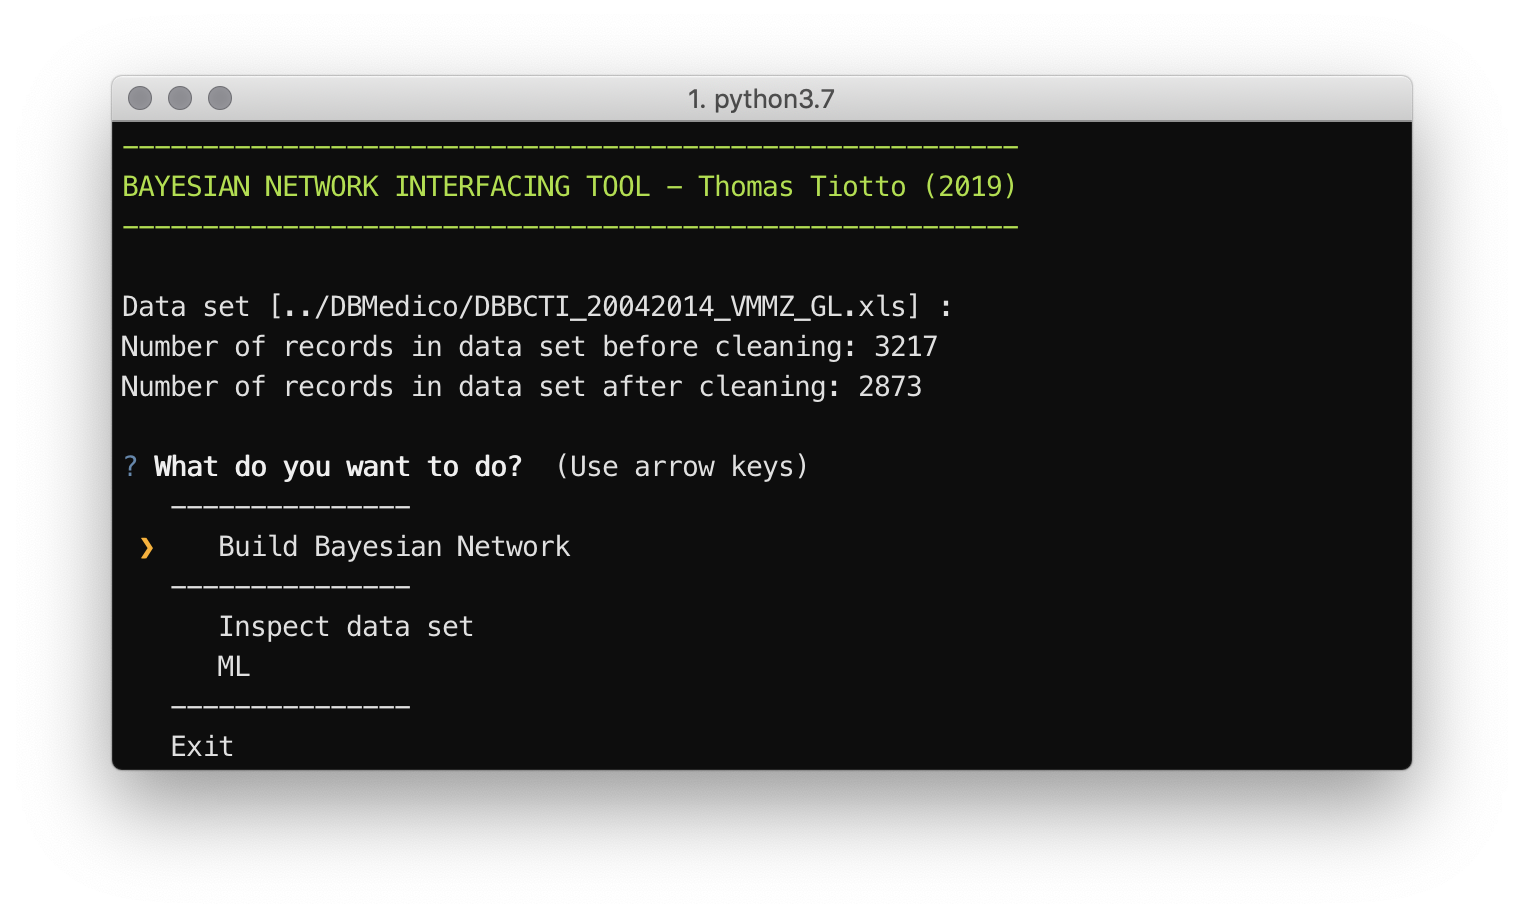
\includegraphics[width=0.7\textwidth]{results/images/sw_0}}
\caption{Initial screen in the developed tool.}
\label{fig:sw_0}
\end{figure}

\begin{figure}[htbp]
\centerline{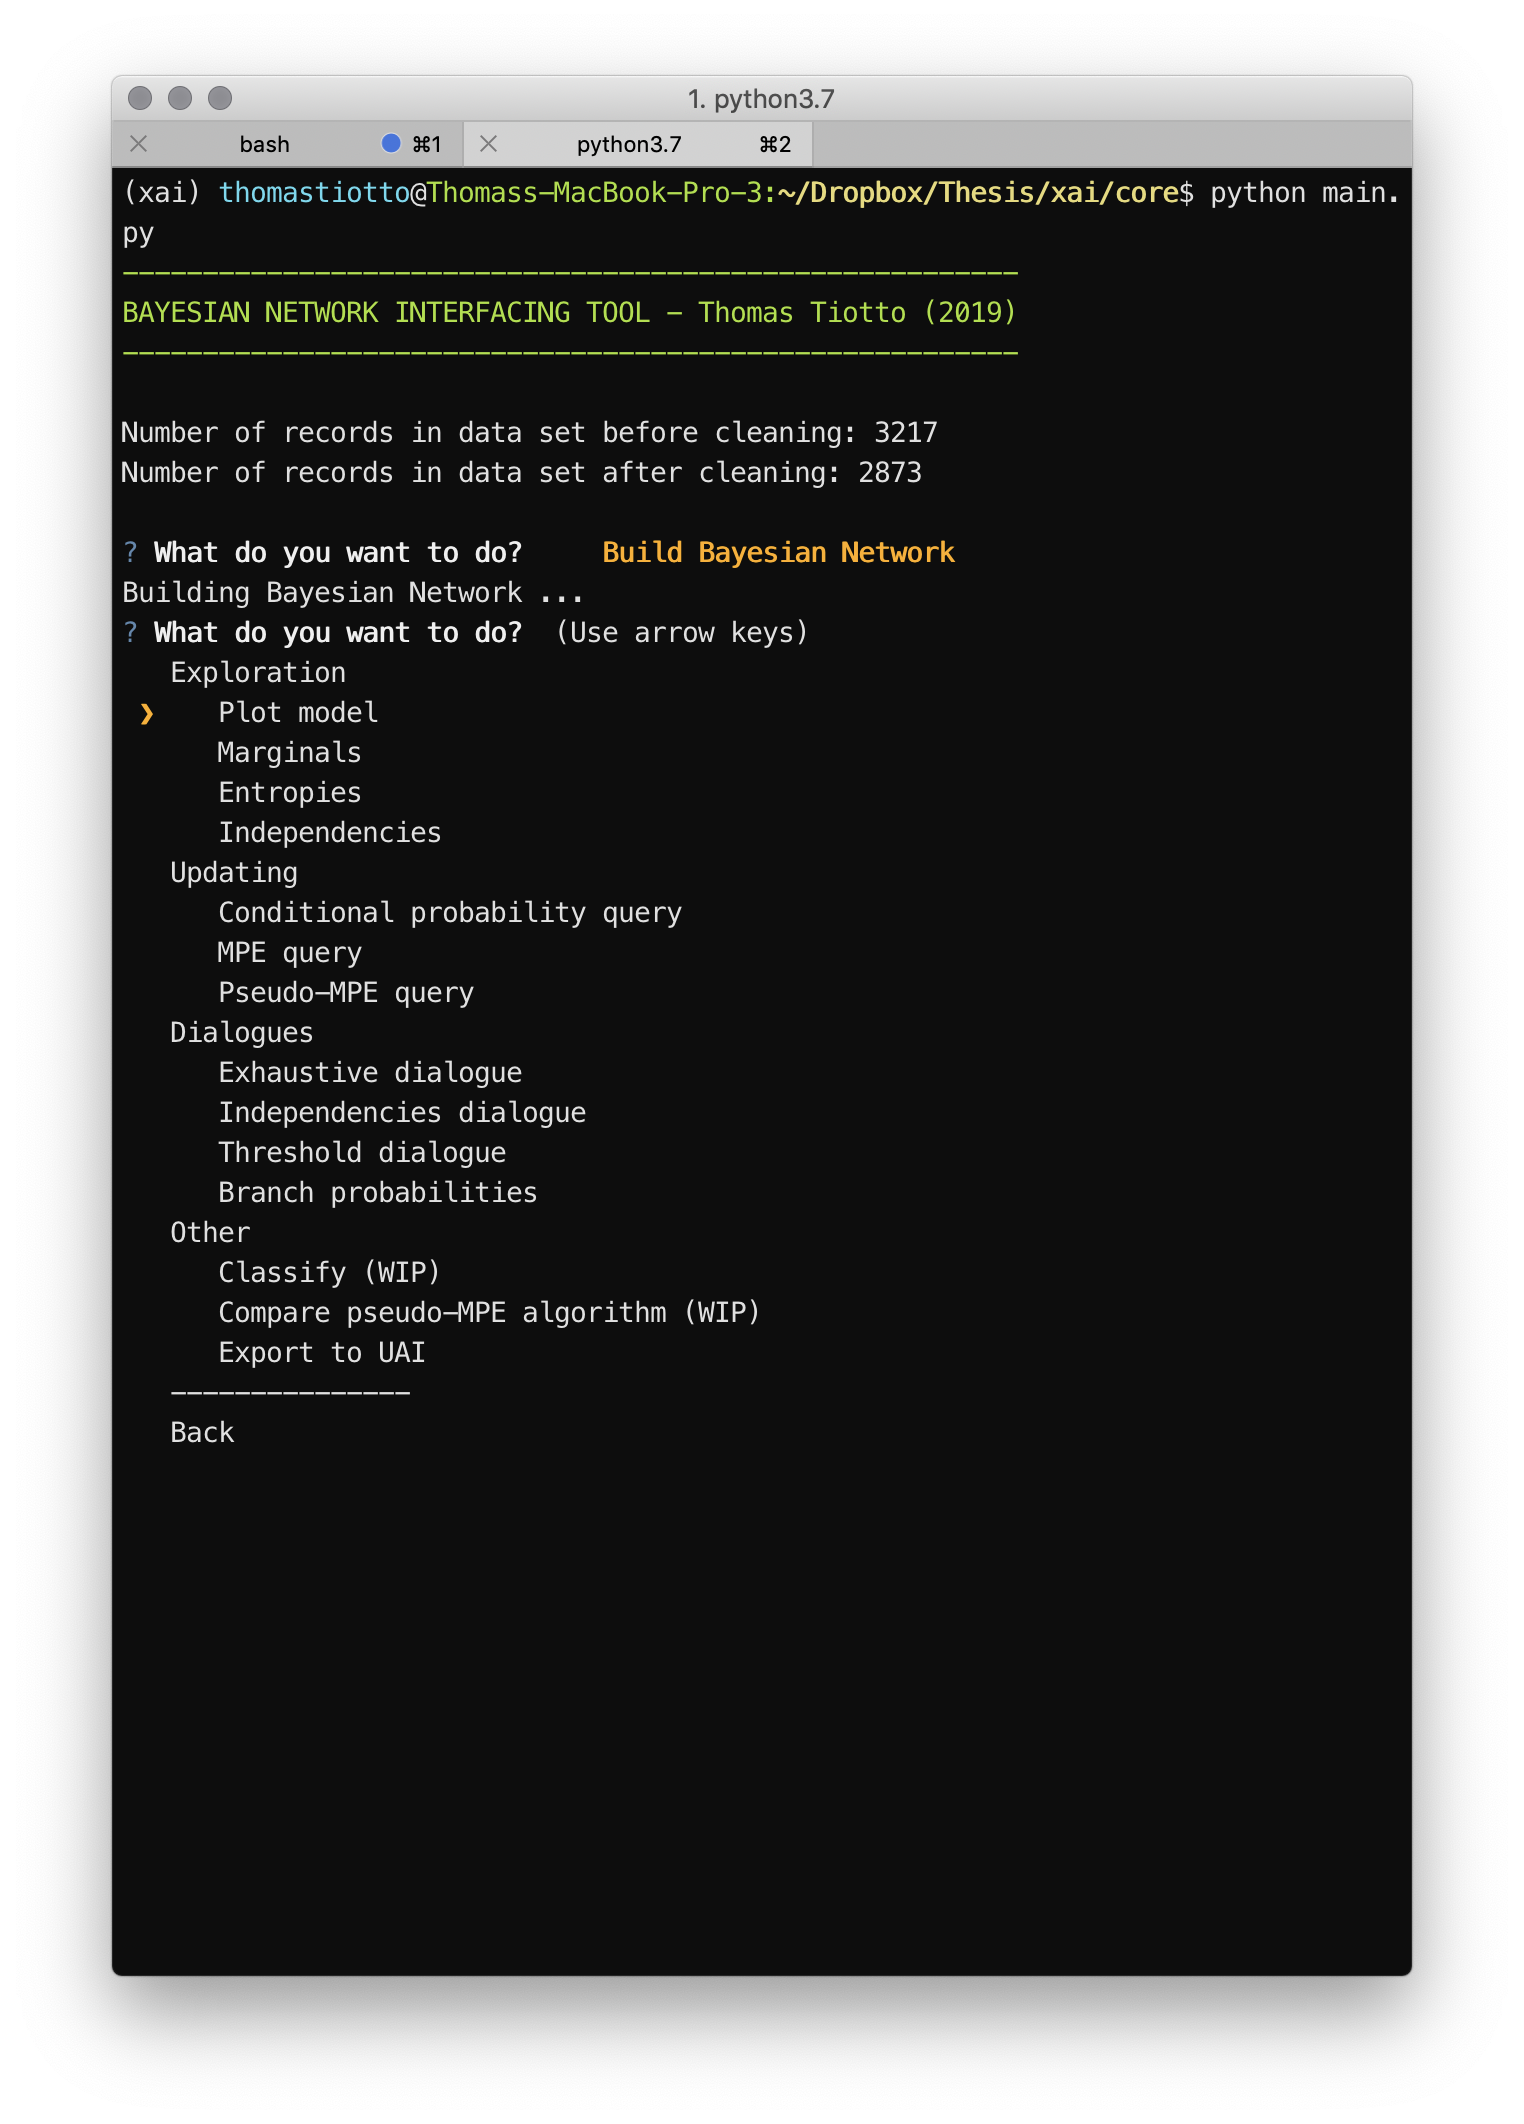
\includegraphics[width=0.7\textwidth]{results/images/sw_1}}
\caption{Main interaction menu.}
\label{fig:sw_1}
\end{figure}

\subsection{Plot Model}
The \enquote{Plot Model} interaction mode would be an example of a \textit{static}, \textit{graphical} explanation in the framework defined by \citet{lacave2002review}, aimed at \textit{explaining the model}.
Compared to the characteristics of an explanation identified by \citet{miller2018explanation}, this might be erroneously regarded as a \textit{causal} explanation. 
Yet, it is important to remember that the directed graphs underlying a Bayesian network are not necessarily describing causal relations, but only probabilistic dependencies.

The \enquote{Plot model} interaction mode gives the expert an overview of the variables present in the system and their relationships by displaying the underlying BN's DAG, with the directionality of edges removed for the reasons explained in \ref{subsec:results-independencies-dialogue}.
Apart from the DAG, mutual information (Definition \ref{def:mutual-information}) between every pair of connected variables is shown on the edges in order to help the expert gauge the strength of the connection.

The users at the ICP considered this interaction modality a good solution to immediately visualise all the features of the data set at a high level together with their relationships; i.e., it gave the user a sense of the \textit{context} of the data set at hand. 
The scaling of the thickness of an edge in a manner proportional to the mutual information of the variables it connects was also considered useful in helping to appreciate the varying strength of the correlations between clinical variables.

The output for the data set presented in Section \ref{sec:data-set} in shown in Figure \ref{fig:sw_plot_result}.

\begin{figure}[htbp]
\centerline{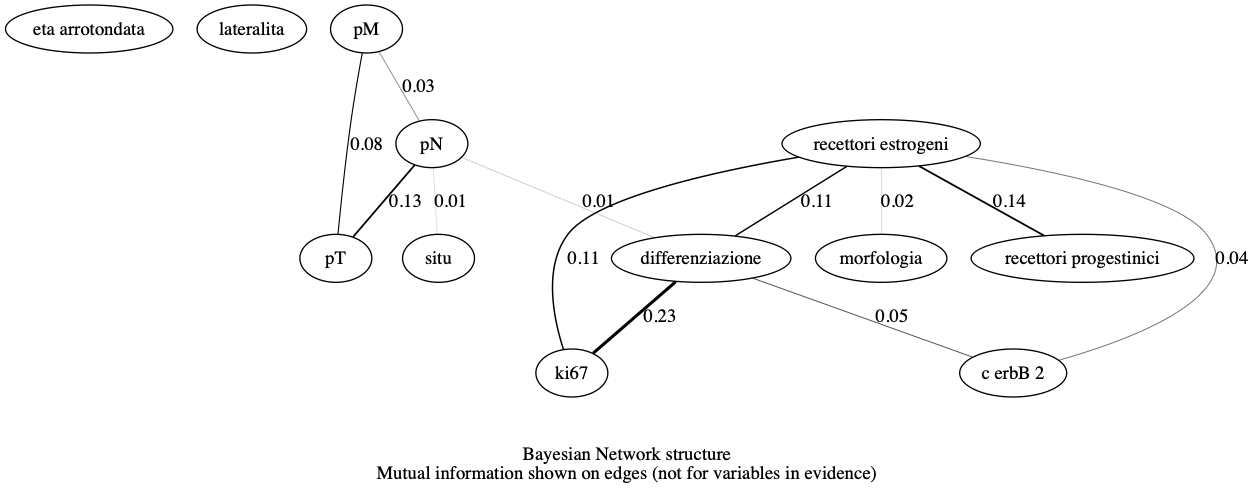
\includegraphics[width=\textwidth]{results/images/plot_result}}
\caption{Plot model output.}
\label{fig:sw_plot_result}
\end{figure}

\subsection{Independencies} \label{subsec:results-independencies-query}
The \enquote{Independencies} interaction mode would be an example of a \textit{static}, \textit{linguistic} and \textit{graphical} explanation in the framework defined by \citet{lacave2002review} aimed at \textit{explaining the model}.
Compared to the characteristics of an explanation identified by \citet{miller2018explanation}, it could be seen as possessing the \textit{selected} and \textit{causal} elements.

The \enquote{Independencies} interaction mode gives the expert the possibility of verifying which d-separations (Definition \ref{def:d-separation}) exist in the constructed Bayesian network's DAG (Definition \ref{def:dag}) .
The concept of d-separation is here reworded into a higher-level notion of \enquote{choosing a source variable and a set of evidence to see which other variables have influence on the source, given the evidence}.
This recasting was deemed necessary because the clinicians at the ICP initially had difficulty in conceptualising at the level of graph theory, probably due to the the misinterpretation of the directionality of the edges in the graphs of a Bayesian network.
Graphs and trees are quite widely-used in clinical practice; however, the presence of an edge is commonly interpreted not as a correlation, but often as an indication of causality. 
Thus, the concept of d-separation could be misinterpreted because of this consolidated viewpoint.
For this same reason, after having chosen first the source variable and then the observed set of evidence variables, the user is presented with an output both in graph (Figure \ref{fig:independencies_output}) and in natural language (Figure \ref{fig:sw_2_independencies}) form.
Having both output modalities present was seen to reduce the confusion that users trained in the medical sciences felt for such an unfamiliar concept.

The new visualisation of d-separation (see Figure \ref{fig:independencies_dialogue_output}), introduced on the basis the the ICP's suggestions, was confirmed by the clinicians to be very intuitive, especially when compared to the initial design (see Figure \ref{fig:independencies_dialogue_output_old}).

\begin{figure}[htbp]
\centerline{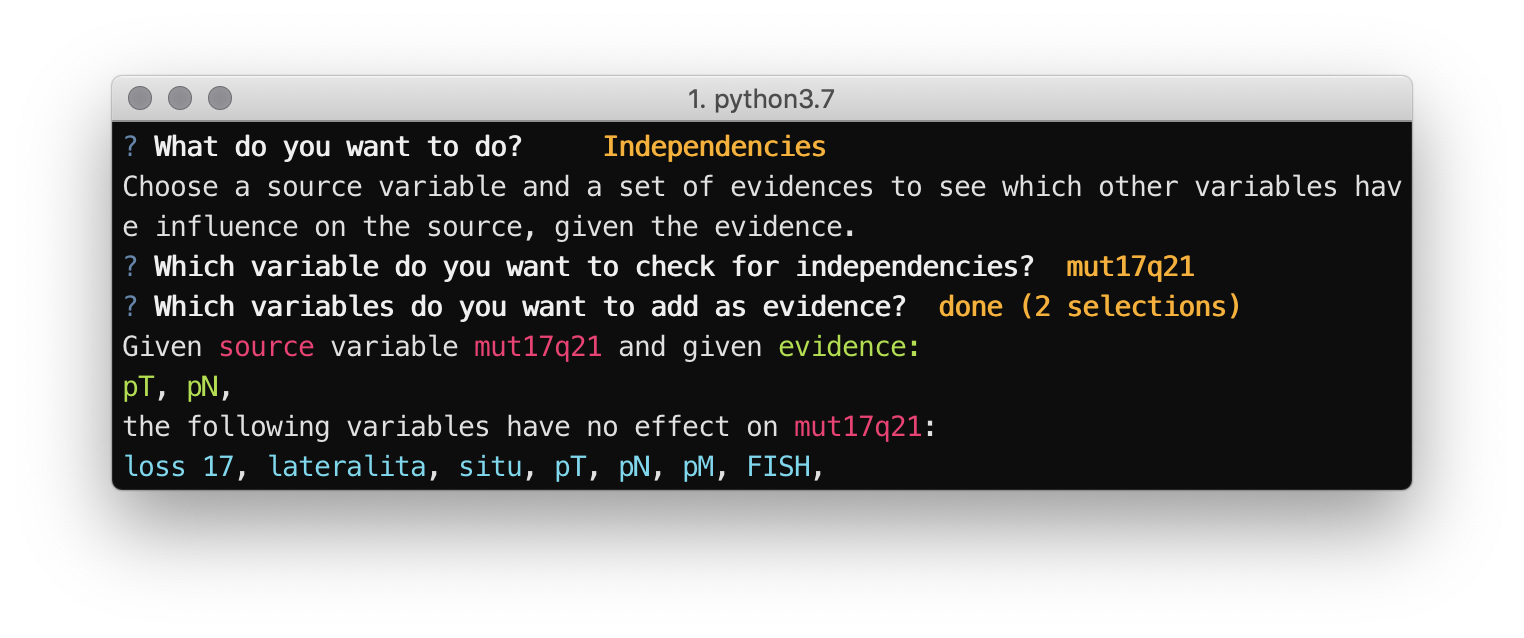
\includegraphics[width=0.7\textwidth]{results/images/sw_2_independencies}}
\caption{Independencies query natural language output.}
\label{fig:sw_2_independencies}
\end{figure}

\begin{figure}[htbp]
\centerline{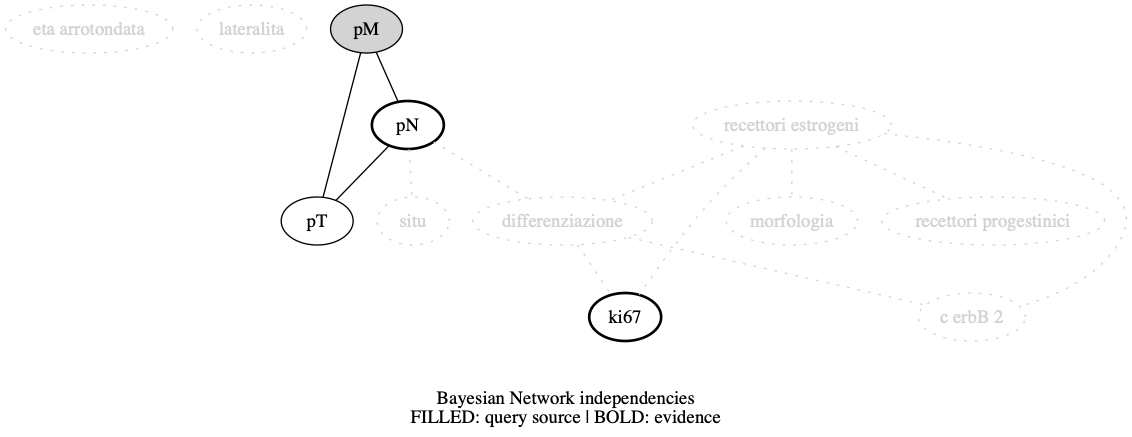
\includegraphics[width=\textwidth]{results/images/independencies_output}}
\caption{Independencies query graph output.}
\label{fig:independencies_output}
\end{figure}

\subsection{Conditional Probability Query} \label{subsec:results-conditional-probability-query}
The \enquote{Conditional Probability Query} would be an example of a \textit{static}, \textit{linguistic} explanation in the framework defined by \citet{lacave2002review} mainly aimed at \textit{explaining the evidence}.
Compared to the characteristics of an explanation identified by \citet{miller2018explanation}, it could be seen as possessing the \textit{selected} element.

Conditional probability queries (Definition \ref{def:conditional-probability}) were seen to be instinctively understood by the clinicians at the ICP.
Indeed, many of the natural language questions that they defined to clinically validate the system (see Subection \ref{subsec:clinical-validation-methodology}) could be framed as and answered by instances of this type of query.

As can be seen in Figure \ref{fig:sw_3_query}, the user is asked for a target variable (in magenta) of which to observe the conditioned values and for a set of variables, together with their observed values (in green).
The output, in natural language, includes all elements of the query together with the colour-coding described in Subsection \ref{subsec:interfacing-user}.
The answer to the question (in cyan), shows the probability of each of the states of the target variable quantified in natural language i.e., as linguistic probabilities, using the coding defined in Table \ref{tab:naturallanguageprobabilities}, and as raw probabilities, shown as percentages.

In addition, the use of colours was appreciated by the users at the ICP because they felt that it helped them to orient themselves among the different elements of the query and also to remember how they had posed it.  

\begin{figure}[htbp]
\centerline{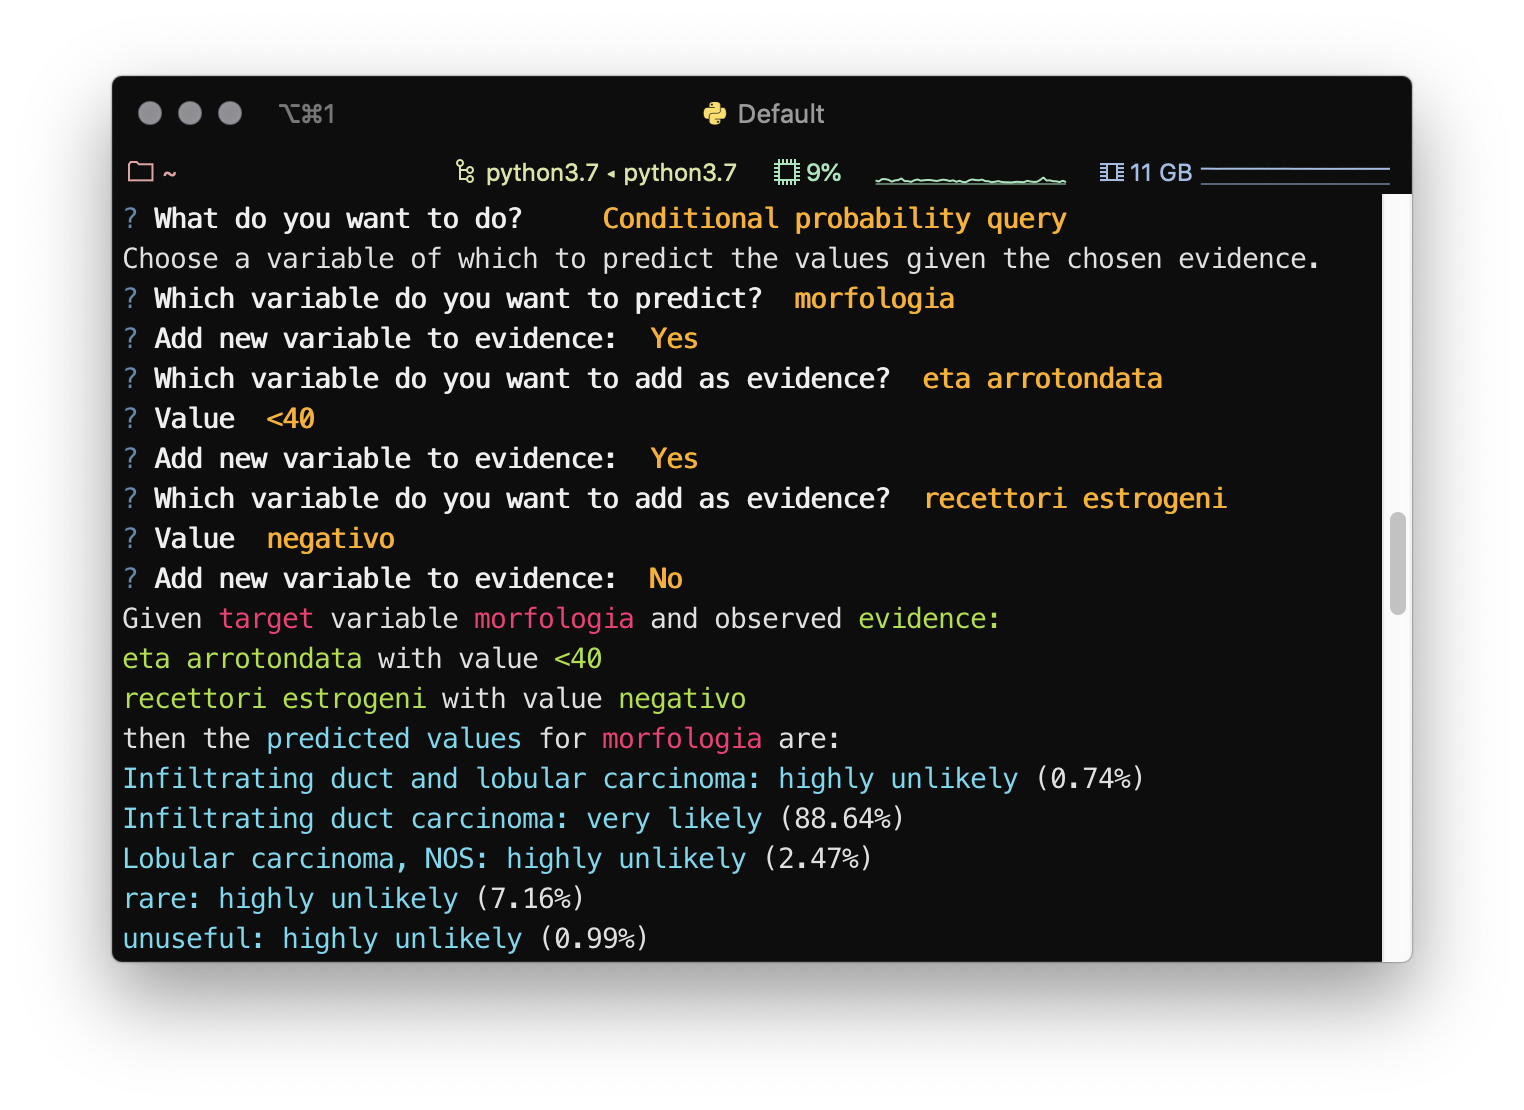
\includegraphics[width=0.7\textwidth]{results/images/sw_3_query}}
\caption{Conditional probability query output.}
\label{fig:sw_3_query}
\end{figure}

\subsection{MPE Query}
The \enquote{MPE Query} would also be an example of a \textit{static}, \textit{linguistic} explanation in the framework defined by \citet{lacave2002review} mainly aimed at \textit{explaining the evidence}.
Compared to the characteristics of an explanation identified by \citet{miller2018explanation}, it could be seen as possessing the \textit{selected} element.

Queries of the MPE type (Definition \ref{def:mpe}) were not initially understood until a bridge to concepts familiar to clinical practitioners had been established.
When presented at an abstract, mathematical level, the experts of the ICP were not sure of the utility of such a query class.
With some work, it was understood that an MPE query could be linked to a concept familiar to any clinician: that of \enquote{a maximally likely patient profile}.
That is, given a set of known parameters it is of interest for the clinician to find which is the most likely assignment to the others.
As each record in the data set represents a patient's clinical profile, this is equivalent to finding the most probable patient given a set of know values.

Another way than an MPE query makes clinical sense, is in the crucial task of predicting missing values for a patient.
This is not an unlikely case, as discussed in Subsection \ref{subsec:motivation}, because there is more than one reason that patients may be missing one or more entries in their clinical profiles.
Executing an MPE query with the known patient's values will yield the most probable assignments to the missing ones and is thus equivalent to a prediction task.
The clinical significance of such an interaction mode can also be inferred from the fact that a number of the natural language questions, that were spontaneously defined to validate the system (see Section \ref{sec:validation}), were seen to map onto instances of this type of query.

At a technical level, the MPE calculation is executed using Pgmpy's \texttt{map\_query} function. 

The output, shown in Figure \ref{fig:sw_4_mpe}, presents, in colour-coded natural language, the input evidence (in green) and most probable assignments to the remaining variables (in cyan).

\begin{figure}[htbp]
\centerline{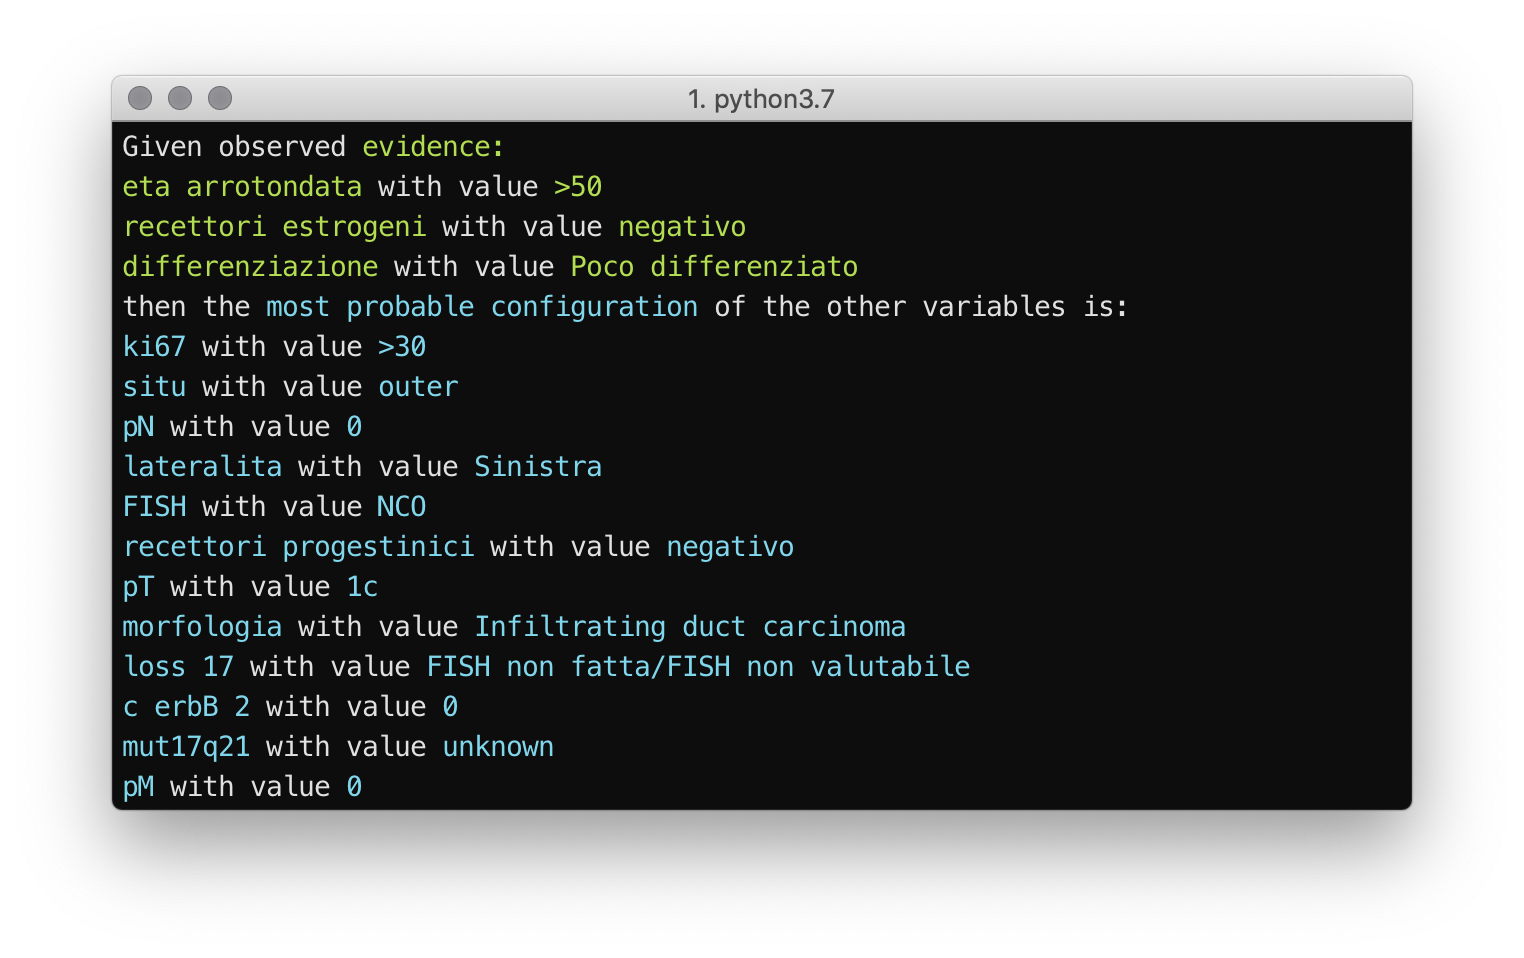
\includegraphics[width=0.7\textwidth]{results/images/sw_4_mpe}}
\caption{MPE query output.}
\label{fig:sw_4_mpe}
\end{figure}

\subsection{Pseudo-MPE Query} \label{subsec:results-pseudo-mpe-query}
The \enquote{Pseudo-MPE Query} would be an example of a \textit{static}, \textit{linguistic} and \textit{graphical} explanation in the framework defined by \citet{lacave2002review} mainly aimed at \textit{explaining the evidence} but also the \textit{reasoning}.
Compared to the characteristics of an explanation identified by \citet{miller2018explanation}, it could be seen as possessing the \textit{selected} and \textit{causal} elements, while remembering that the implications resulting from a BN are not necessarily causal.

The \enquote{pseudo-MPE query} interaction mode is aimed at generating a \enquote{maximally probable} assignment using the methods described in Subsection \ref{subsec:algorithms-novel} under the \enquote{pseudo-MPE from Initial Evidence} header.
The hypothesis is that this should be a valid explainability tool, as it is not only a \textit{linguistic} but also a \textit{graphical} explanation, with the latter element being identified by \citet{lacave2002review} as one of the most effective ways of giving a satisfactory explanation in a BN.\footnote{If the cardinality of the set of variables to explain is one, i.e., $|E| = |V|-1$, with $E$ the evidence set and $V$ the set of variables in the BN, then the \enquote{pseudo-MPE} and true MPE assignments will be identical.}

The user is first asked for the probability threshold under which to discard the \textit{(state,value)} pairs whose probability is deemed too low.
Then, after being asked for the initial observed evidence, the expert is presented with the constructed polytree (Definition \ref{def:polytree}); an output example can be seen in Figure \ref{fig:pseudo_mpe_output}.
This polytree will have the initial evidence, that the expert specified, as roots and a single chain of \textit{(state,value)} pairs, each one quantified with its probability (in natural language) given all of its ancestors.

A doubt, that presented itself quite early during the ICP's evaluation, concerned the quantification of probabilities in the chain.
The pathologists were unsure of why \textit{(state,value)} pairs appeared before others that had been reported as more probable.
For example, in Figure \ref{fig:pseudo_mpe_output}, \textit{(\enquote{morfologia},\enquote{Infiltrating duct carcinoma})} that is considered \textit{likely} appears before \textit{(\enquote{recettori estrogeni},\enquote{fortemente positivo})} which is considered \enquote{very likely}.
The pathologist's intuition brought her to expect this deduction chain to be monotonically decreasing in probability from the initial evidence (that, as such, is certain).

What turned out to be the point of confusion, was that it was unclear that the probability of every node added to the chain depends on all its ancestors.
In the specific example, \textit{(\enquote{recettori estrogeni},\enquote{fortemente positivo})}'s evidence set also contains \textit{(\enquote{morfologia},\enquote{Infiltrating duct carcinoma})}.
There is thus, mathematically, no reason for the chain to be monotonically decreasing in probability because adding new evidence is liable to boost the likeliness of some unobserved variables.
Returning to the example, the marginal probability $\mathbb{P}((\text{\enquote{recettori estrogeni},\enquote{fortemente positivo}}))$ may very well have been less probable than \enquote{very likely}, maybe it was only \enquote{likely} or even \enquote{unlikely}, but this says nothing about the posterior probability $\mathbb{P}((\text{\enquote{recettori estrogeni},\enquote{fortemente positivo}}) \mid (\text{\enquote{morfologia},\enquote{Infiltrating duct carcinoma}}) )$, which is what the polytree displays.

The unclearness of the chain of inferences is certainly not a point to underestimate, as the hope was for the \enquote{pseudo-MPE} output to be able to clarify the underlying reasoning process of the models and thus help in guiding the expert's through process.
If this reasoning process itself were unclear, this could hardly lead to a good explanation; thus an effort will have to be made to explain the underlying assumptions better, while also being mindful when evaluating if this output mode genuinely presents the characteristics of a good explanation.

\begin{figure}[htbp]
\centerline{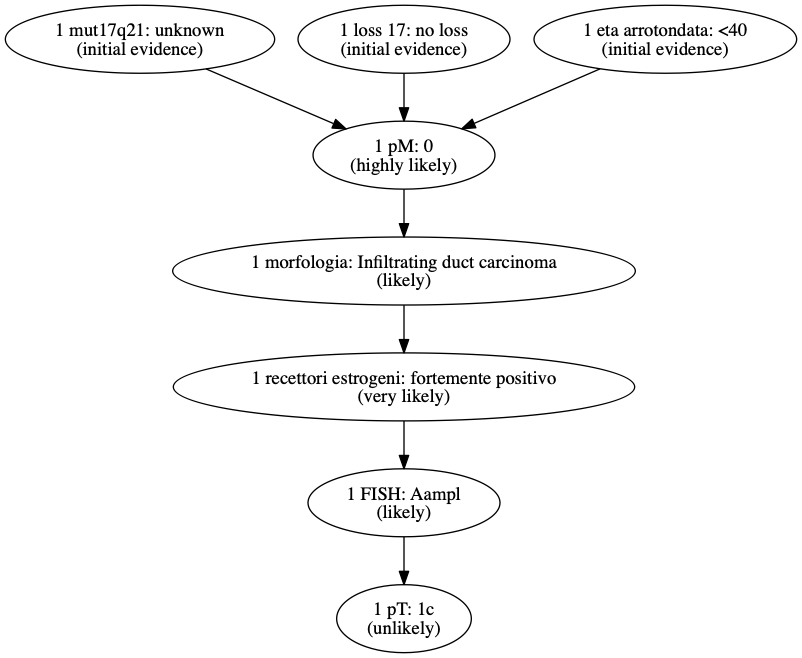
\includegraphics[width=0.7\textwidth]{results/images/pseudo_mpe_output}}
\caption{Pseudo-MPE query output with threshold $0.5$.}
\label{fig:pseudo_mpe_output}
\end{figure}
%
%\subsection{Belief revision}
%\todo[inline]{da lasciare?  da espandere?  da spostare?}
%Philosophically, what is being done during the dialogues is a process of \textit{hard belief revision}.
%This is because the expert's choice is taken by the system as absolute truth and added to the previous evidence set.
%
%The process of \textit{belief revision} is distinct from that of \textit{belief updating} as in the latter previous beliefs are updated to conform to new information received.
%Belief revision on the other hand does not modify previous evidence, as this is simply supposed to be less reliable than the newer one.
%This last setting is the one that happens during the dialogues, because previous \textit{(state,value)} tuples are not modified in their probabilities given the new evidence supplied when the expert accepts a proposal.
%We talk about \textit{hard} belief revision because the new evidence generated by the user is treated as if it were certain - i.e., with probability 1 - and added to the evidence set without creating inconsistencies.
%\todo[inline]{come si potrebbe giustificare?  ha senso tenere il paragrafo?}

\subsection{Exhaustive Dialogue} \label{subsec:dialogue-results}
The three dialogue variants would be examples of \textit{dynamic}, \textit{contrastive}, \textit{linguistic} and \textit{graphical} explanations in the framework defined by \citet{lacave2002review} aimed at \textit{explaining the evidence} but also, and most importantly, to \textit{explaining the reasoning}.
Compared to the characteristics of an explanation identified by \citet{miller2018explanation}, these could be seen as possessing all the necessary elements: \textit{contrastive}, \textit{selected}, \textit{causal} and \textit{social}.

The three \enquote{dialogues} are the most experimental interaction modes and thus also the most alien to a user.
None of the natural language questions defined by the ICP in the form described in Subsection \ref{subsec:clinical-validation-methodology} could be directly mapped onto such a dialogical process.
On the other hand, the dialogue aims to build an \textit{expert-driven MPE approximation} and could thus be regarded as essentially answering the same question as the \enquote{pseudo-MPE} and \enquote{MPE} queries (Subsection \ref{subsec:results-pseudo-mpe-query}).
The research hypothesis is wether this could be a better explainability tool, as it is not only a \textit{linguistic} and \textit{graphical} explanation but also a \textit{dynamic dialogue} that \citet{Hilton1990} and \citet{lacave2002review} identify as a key ingredient in having an effective explanation.
Another important fact is that the dialogues offer a \textit{counterfactual} branch when the expert dissents with the model; \citet{miller2018explanation} singles out being \textit{contrastive} as one of the defining characteristics of an effective explanation, as this feature closely aligns with our expectations of what an explanation should entail.

Because of the novel nature of such a knowledge-extraction process, three different versions were implemented with each one adding a different set of behaviours to the \enquote{exhaustive} version described in this subsection.
This helped in exploring the space of possibilities and aided in understanding which features were preferred by the clinicians of the ICP, both as a means for knowledge-extraction from the data set and from a comprehensibility point of view.
It should here be noted that comprehensibility of the outputs is a \textit{necessary} but \textit{not sufficient condition} to be able to gain knowledge from data.
Both variants to the basic dialogue - the independencies-aware and the thresholded one - aim to prune the space of variables proposed to the user in order to reduce her cognitive load.
This is in keeping with the insight by \citet{miller2018explanation} that explanations are \textit{selected}, meaning that we humans expect that the explaining factors be picked based on some criterion.

The \enquote{exhaustive dialogue}, as described in much more detail in Subsection \ref{subsec:algorithms-novel} under the \enquote{Dialogues} header, is so named because it ends only when the expert user has reviewed all the variables present in the data set.
It starts by asking the clinician for a set of initial evidence and from thereon after iteratively proposes the \textit{(state,value)} pair with the least entropic \textit{state}, based on the accumulated evidence (the rationale behind this is explained in Subsection \ref{subsec:entropy-based-selection}).
An example of such an ongoing interaction is shown in Figure \ref{fig:sw_5_exhaustive_dialogue}.

An issue that was highlighted early on was that the experts had great trouble in building the \textit{knowledge base} from a single evidence; this was the driving motive that pushed the representation of the \enquote{pseudo-MPE} branch beyond a simple \textit{tree} (Definition \ref{def:tree}) - as in \citep{Butz2018} - but towards a \textit{polytree} (Definition \ref{def:polytree}).
This way the expert is able to inject the query with as much domain knowledge as she feels comfortable with.
It was an unrealistic assumption to expect a domain expert to bear the cognitive load of selecting a \textit{single best initial evidence}; this would be a hard task to do in its own right but it is made even more difficult by the fact that the subsequent dialogue \textit{depends} on the initial evidence.
To effectively select one best evidence, the expert should also have been able to \textit{predict} how the dialogue would have evolved from that initial point onwards.
The dialogue is an \textit{exploratory tool} that the user utilises with the objective of extracting knowledge from the data set; expecting the user to already know the outcome of her choices would mean that she already had the domain knowledge necessary to predict the consequences of those same choices; a clear instance of \textit{circular reasoning}.
This was confirmed by the ICP: having multiple initial evidence helped the users because it reduced the number of tuples proposed by the system and therefore the quantity of choices the users were tasked to deal with.

The general feeling being echoed by the users at the ICP was that the dialogue was the hardest interaction mode to understand and to utilise.
The way they used the dialogues was by nearly always replying \enquote{yes} to its proposals, because they were mostly interested in seeing what the machine would propose.
Nonetheless, the users understood the high potential of this method especially when applied with the objective of conducting research, but they reported they would need to \enquote{trust} the interaction mode before feeling comfortable with using it in such a manner.
They felt that probably having more time to experiment with this kind of interaction might improve their confidence felt in using it, that was lower than that perceived for the other interaction methods.

\begin{figure}[htbp]
\centerline{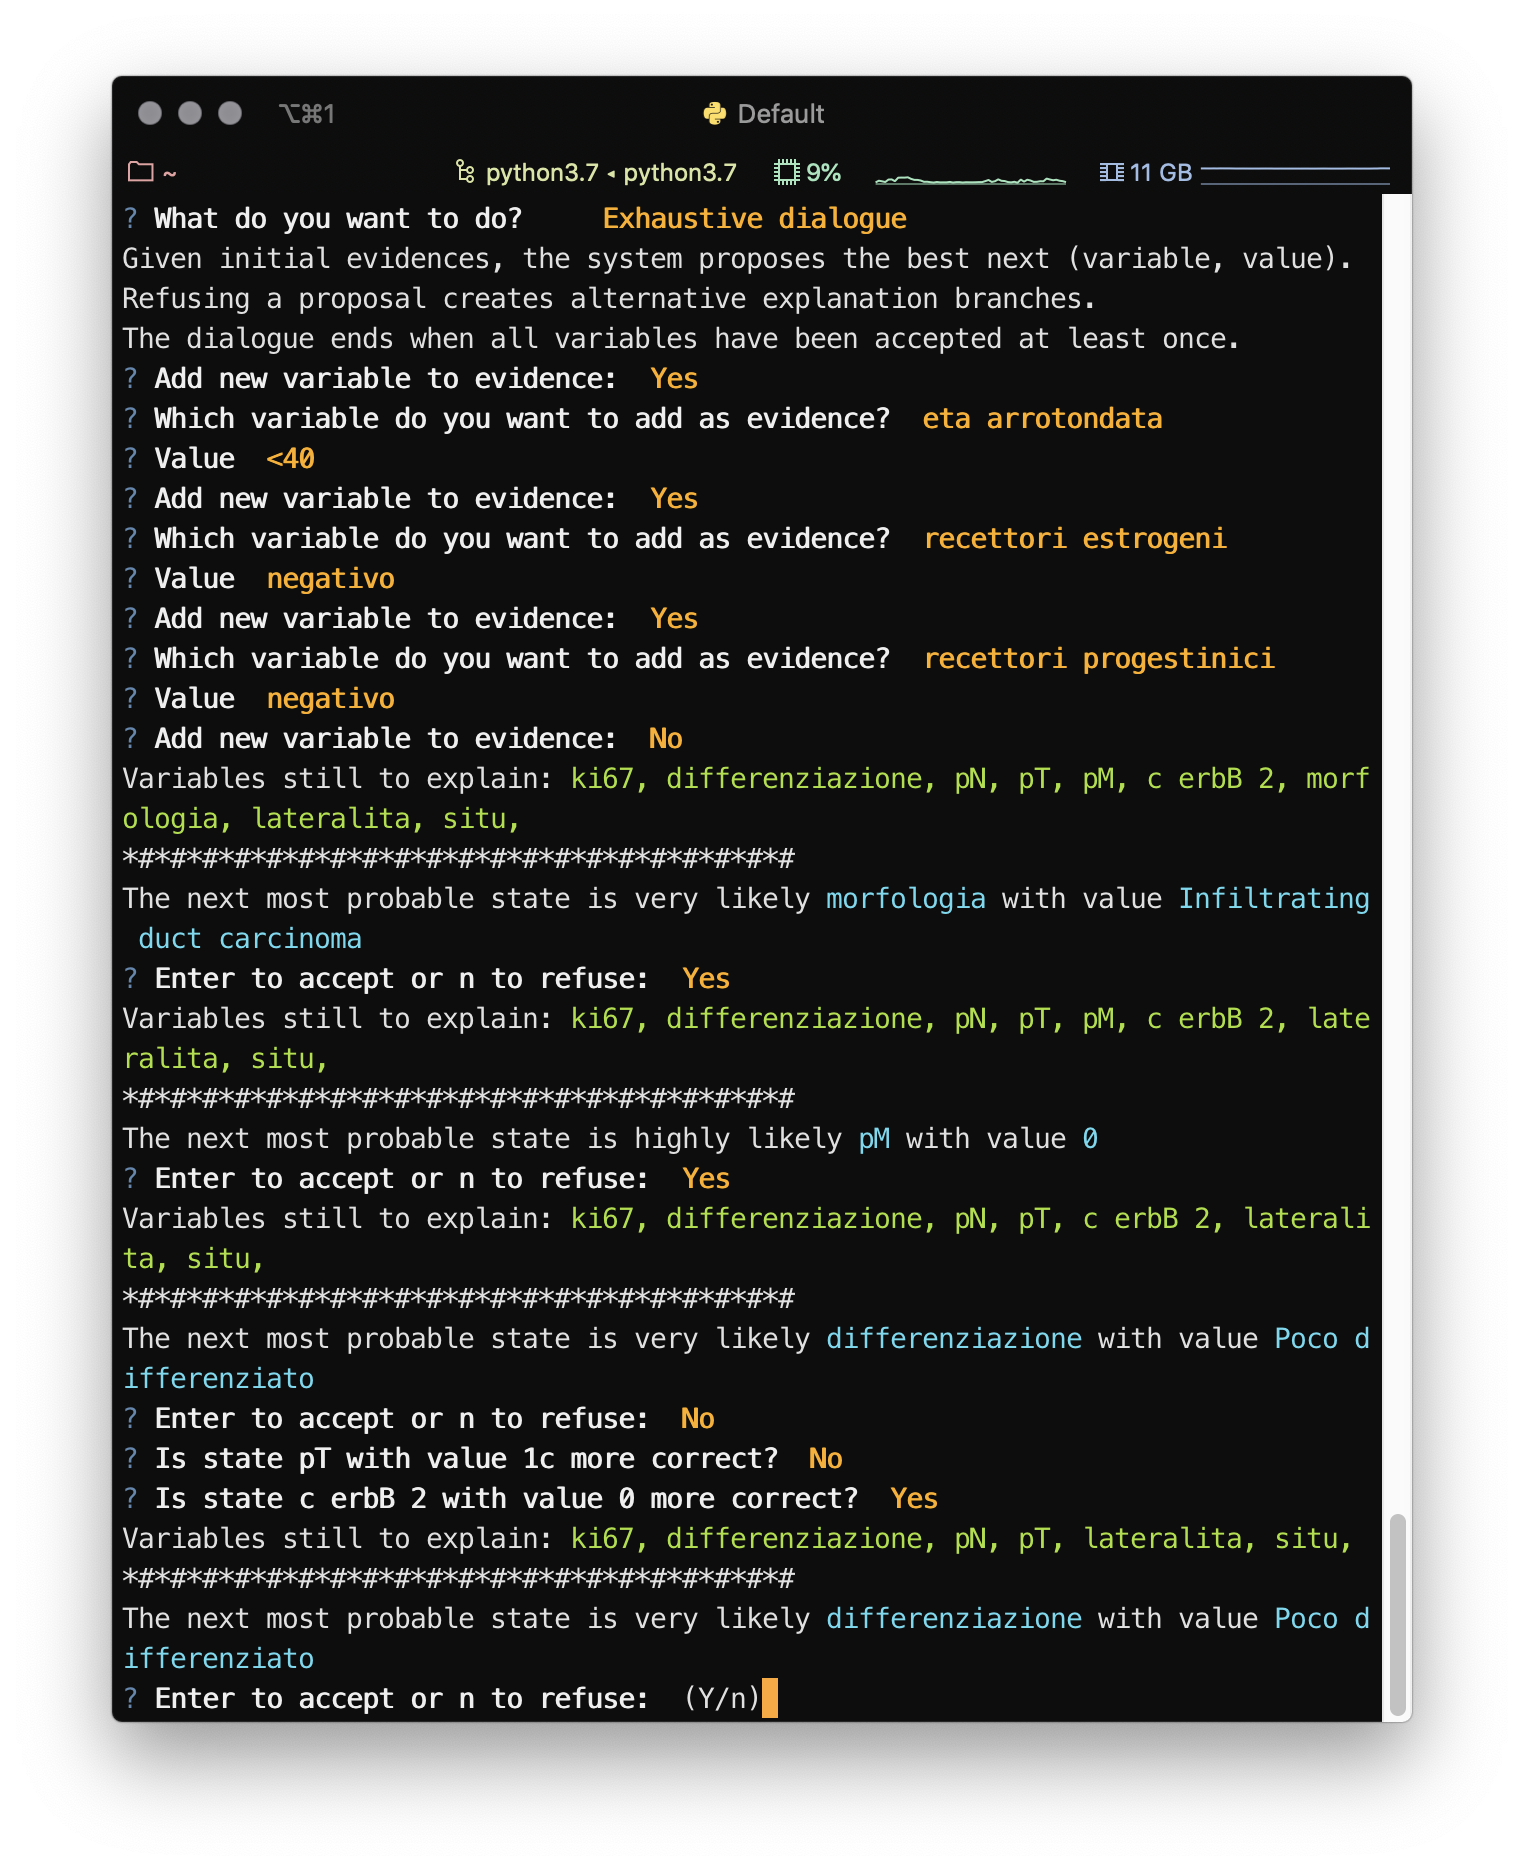
\includegraphics[width=0.7\textwidth]{results/images/sw_5_exhaustive_dialogue}}
\caption{Ongoing Exhaustive Dialogue.}
\label{fig:sw_5_exhaustive_dialogue}
\end{figure}

\subsection{Independencies Dialogue} \label{subsec:results-independencies-dialogue}
The first variant to the \enquote{exhaustive dialogue} takes the approach of excluding variables based on their d-separation properties (Definition \ref{def:d-separation}) in the underlying DAG (Definition \ref{def:dag}).
Thus the cardinality of the set of variables proposed to the user varies in a non-linear way, depending on the topology of the graph and the order of insertions into the evidence set.
In the \enquote{exhaustive dialogue}, presented under the previous header, the relationship between the set of variables still to explain at step $t$, $W_t = V \setminus E_t$, with $V$ all the variables and $E_t$ those already added to evidence, obeys the recurrence relation:
\begin{align}
\begin{split}
		W_0 := V, \\
	E_0 := \emptyset, \\
	|W_{t+1}| = |W_t| - 1, \\
	|E_{t+1}| = |E_t| + 1.
\end{split}
\end{align}
That is, at each step $t$ of the \enquote{exhaustive dialogue}, one variable moves from the set still to explain $W$ to the explained one $E$ i.e., after any iteration step, the number of instantiated variables increases by one unit, while the number of variables to explain also decreases by one.
In the \enquote{independencies dialogue}, this relationship depends on the set of variables $Z$ that are d-separated from those already in $E$.
The relationship between the cardinalities is modelled by an operator $\zeta$ that is unique to the DAG of the BN (or to any \textit{i-equivalent}\footnote{I-equivalence identifies classes of graphs that present the same d-separation properties.} one):
\begin{align}
\begin{split}
	W_0 := V, \\
	E_0 := \emptyset, \\
	|W_{t+1}| = \zeta(|E_t|), \\
	|E_{t+1}| = |E_t| + 1.
\end{split}
\end{align}
As d-separation is not monotonic (adding a variable to $E$ may open new paths and d-connect new variables), the cardinality of the set $W$ may vary, from the point of view of the user, in an unpredictable manner.
To attempt to offset this effect, during the dialogue the user is supported by an updated view of the independencies in the graph (an example during the dialogue is shown in Figure \ref{fig:independencies_dialogue_output}).

Before receiving feedback from the ICP, the visualisation of the independencies was the one shown in Figure \ref{fig:independencies_dialogue_output_old}.
The most striking difference was the use of colour-coding to identify the role and the separation of variables with pink identifying the query variables, blue the evidence, red the separated variables and green the connected ones.
As already noted in Subsection \ref{subsec:results-independencies-query}, the concept of d-separation turned out to be quite unfamiliar to the clinicians of the ICP so the first priority was to represent the concept visually in the clearest way possible.
This was achieved, and confirmed in its efficacy by the pathologists, by fading the separated variables and marking those in evidence in bold, as can be seen in Figure \ref{fig:independencies_dialogue_output}.
The fading of separated variables was felt to successfully reinforce the concept of these not influencing the remaining ones and its directness was especially appreciated.

The use of directed arcs to represent the DAG raised another critical issue that hadn't been foreseen.
In the visual representation of a Bayesian network, an arc between two variables represents a correlation between their values while the direction identifies the \textit{parent} and the \textit{child} in the relationship; for example the graphical representation $X \rightarrow Y$ means that $X$ is the parent of $Y$.
This is a defining characteristic of such a model, because the fundamental idea of a BN is to factorise the joint distribution such that each variable's values depend only on that of its parents; the concept of conditional probability table is explained in Section \ref{sec:bayesiannetworks} and some more examples can be seen in Subsection \ref{subsec:algorithms} under the \enquote{MPE} header.
Nonetheless, the pathologists explained that the DAG representing a BN is very similar to diagrams used during clinical research, with the crucial difference that in those a directed arrow represents \textit{causation} and not \textit{correlation}.
In these diagrams a correlative relationship would have usually been represented by an undirected edge.
For this reason the DAG representation of the BN was \textit{disoriented} in all visualisations.
The ICP confirmed that this new formulation was more closely aligned with the intuition that could be expected by a clinician.

The third element of difference, is the addition of the mutual information coefficient (Definition \ref{def:mutual-information}) on the arcs connecting each couple of variables; the coefficient also scales the width of its associated edge, giving further visual feedback to the user.
This functionality was a direct request from the ICP's representatives since after inspecting the initial DAG visualisation they felt the need for a feature that would increase their understanding of the relationships between the variables.
D-separation is binary while mutual information can give the practitioner a much wider (theoretically infinite) range of information.
For example looking at Figure \ref{fig:independencies_dialogue_output} it is quite easy to see that, while \enquote{morfologia} and \enquote{recettori estrogeni} are d-connected, the amount to which they influence each other's values is small compared to other connected variables.
Some arcs are missing the mutual information coefficient because one of the two variables is in the evidence set, e.g., those belonging to \enquote{recettori estrogeni}.

\begin{figure}[htbp]
\centerline{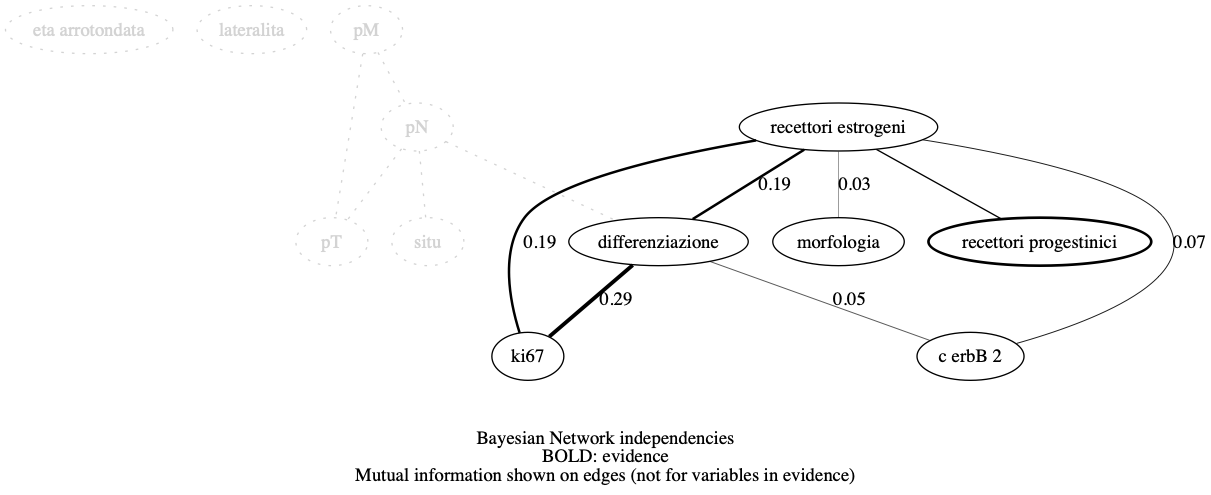
\includegraphics[width=\textwidth]{results/images/independencies_dialogue_output}}
\caption{Ongoing Independencies Dialogue.}
\label{fig:independencies_dialogue_output}
\end{figure}

\begin{figure}[htbp]
\centerline{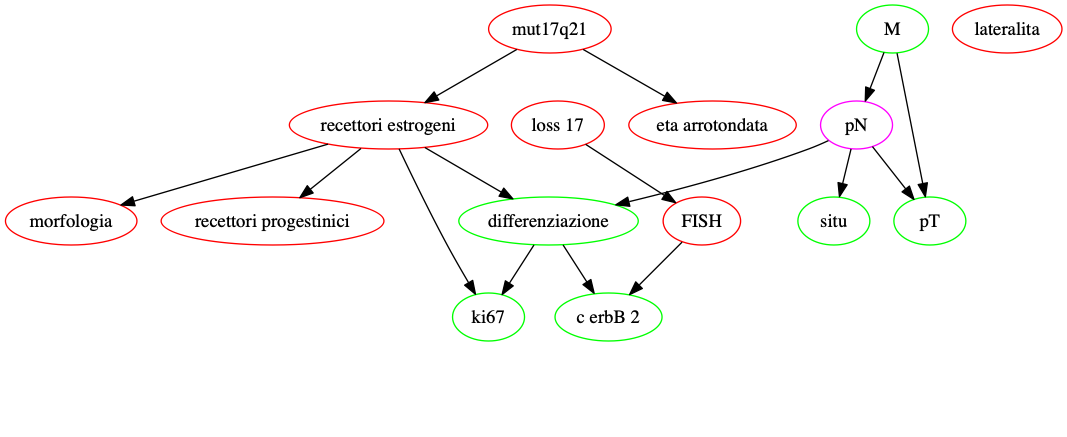
\includegraphics[width=\textwidth]{results/images/independencies_dialogue_output_old}}
\caption{Previous visualisation during Independencies Dialogue.}
\label{fig:independencies_dialogue_output_old}
\end{figure}

\subsection{Thresholded Dialogue}
The final \enquote{dialogue} variant adopts a different strategy for pruning; namely one based on the probability of the proposed tuples and on the number of times they have been refused by the expert.
This implements a suggestion found in \citet{lacave2002review} that explanations should be graded on the user and not on a \textit{fixed user model}; one of the ways this has been addressed in literature is by the introduction of thresholds to filter unwanted information.

The cardinality of the set $W$ of states to explain decreases linearly, similarly to the \enquote{exhaustive dialogue}, but potentially with a slope coefficient $\alpha \leq -1$, as many states may be infra-threshold i.e., too improbable to be considered.
Unlike the independencies dialogue, the cardinality of $W$ cannot increase:
\begin{align}
\begin{split}
	W_0 := V, \\
	E_0 := \emptyset, \\
	|W_{t+1}| = \alpha |W_t|, \\
	|E_{t+1}| = |E_t| + 1.
\end{split}
\end{align}
The default values for the threshold and the maximum number of times a \textit{(state, value)} tuple could be proposed were decided together with the ICP and set to:
\begin{itemize}
  \item \textit{threshold}: 0.4, a \textit{(state, value)} tuple is ignored if the probability of \textit{value} is less that 0.4;
  \item \textit{refusal limit}: 2, a \textit{(state, value)} is ignored if it has already been refused twice.
\end{itemize}
\section{Validation Results} \label{sec:results-validation-results}
This section will present the clinical and explainability results of the developed system, based on the methods outlined in Section \ref{sec:validation}.

\subsection{Domain Experts' Initial Expectations for an Explanation} \label{subsec:domain-experts-initial-expectations}
At the beginning of this project, it was not easy for the ICP's experts to understand what AI was exactly and how an interactive tool in this domain could look like.
For these reasons, they considered the idea of receiving an output in natural language highly intriguing, as this was the output modality they had the most experience working with.

Because of the novelty of the approach developed in this thesis as applied to the field of medicine, the experts were open to receiving many different types of explanation, for example, textual, graph-based or tables.
Nonetheless, in their mind, the preferred one would still be a natural language output, as they imagined it as being much simpler, clearer and compact than any other output modality.
Thus, their ideal explanation would be a natural language output that were corroborated by the values in the data, presented a summary of their inputs to the system (for example, the used query and evidence variables) and that were understandable in terms of probability.

The ICP representatives felt that their preference for \textit{verbal} explanations over any other form, stemmed from a \textit{forma mentis} ascribable to the fact that nearly all medical literature is highly verbal in the way it communicates content; tables are little used and graphs are often ignored because there is little standardisation in the way they are presented across the subfields of the medical domain.
Clinicians thus prefer to focus on reading the textual, conversational description that accompanies the results presented and this habit has shaped their expectations of what an explanation should look like.

\subsection{Clinical Validation} \label{subsec:clinical-validation-results}
\subsubsection{Natural Language Questions Results}
The natural language questions marked as \textit{validation}, that were presented in Subsection \ref{subsec:clinical-validation-methodology} have been discussed and validated by Dr. Vittoria Martin, molecular cytogeneticist at the ICP (see Subsection \ref{subsec:istituto-cantonale}), and Dr. Luca Mazzucchelli, director of the ICP. 
The questions tagged as \textit{research} necessarily have an \textit{unknown} \textit{Expected result} but, as noted in Subsection \ref{subsec:clinical-validation-methodology}, are nonetheless extremely interesting in order to understand how the user relates to the system.
The system's outputs to their questions are shown together with the results they would have expected, based on established medical literature and their professional expertise.
The ICP representatives had the faculty to \textit{agree} or \textit{disagree} with the software's judgement and, where they felt it necessary, were able to leave notes, that have also been reported in this section.

Tables \ref{tab:resultsconditionalquestions}, \ref{tab:resultsdseparationquestions}, \ref{tab:resultsdseparationquestions} and \ref{tab:resultsdseparationquestions} present the clinical validation results for the natural language questions in Annexes \ref{ann:conditionalprobability1}, \ref{ann:conditionalprobability2}, \ref{ann:dseparation}, \ref{ann:conditionalanddseparation} and \ref{ann:mpe}. 
Table \ref{tab:recapquestionsresult} shows the experts' comments in aggregated form by summing the number of times the comment appeared over the thirty questions.
Comments followed by \enquote{to further explore} were aggregated except for question number 4 where \enquote{agree, to further explore} was also counted in \textit{agree}.
Note that questions 12 and 13 are compound, that is they were run multiple times by changing the \textit{evidence values} for the same \textit{evidence variable.}

Table \ref{tab:recapquestionsresult} strongly supports the idea that the developed system, and by extension the underlying Bayesian Network, is able to capture the clinical relevance of the variables in the data set, in the current application domain.
Twenty-four query answers out of a total of thirty-five found the ICP experts as either in \enquote{full agreeance} of in \enquote{agreeance} with the system's predictions while one was deemed \enquote{acceptable}.

Three queries (numbers 23, 25 and 27 in Annex \ref{ann:conditionalanddseparation}) were not executed by the domain experts; this is because they had framed them as conditional probability queries but these were, in actuality, questions that could have easily been answered by d-separation queries.
For example, question number 23 reads:
\begin{quotation}
	In young patients, does a negative expression of the progestinic receptors influence the lymph nodes' state?
\end{quotation}
Framing this as a conditional probability query would mean having to obtain the value of \enquote{lymph nodes' state} (\enquote{pN} in the benchmark data set) for all the combinations of values of \enquote{age} and \enquote{progestinic receptors} (\enquote{eta arrotondata} and \enquote{progestinici} in the data set) in order to see if a change in the latter produced a variation in the former.
Instead, a d-separation query can directly answer if the nodes of the variables representing \enquote{lymph nodes' state} are d-separated from those for \enquote{age} and \enquote{progestinic receptors}.
The answer given by the d-separation query is less informative than that of a conditional probability query in case the nodes are not d-separated, but nonetheless answers the question as it was posed.
This misunderstanding of the use of the tool is certainly to take note of but the instances of confusion are also limited to only a particular phrasing of question among all those posed.
As such, it could probably be addressed by tweaking the information presented to the user.

The answers to the remaining nine questions were not excluded \textit{a priori} by the ICP's representatives but were deemed interesting enough \enquote{to further explore}.

\begin{table}[h]
	\centering
	\caption{Aggregation of expert answers}
	\begin{tabularx}{0.7\textwidth}{lXl}
		\toprule
		& Expert comment & Counts  \\
		\midrule	
		& fully agree & 4 \\
		& agree & 20 \\
		& acceptable & 1 \\
		& to further explore & 9 \\
		& query not executed & 3 \\	
		\midrule
		\textbf{Total} & & 35 \\
		\bottomrule
		\end{tabularx}
	\label{tab:recapquestionsresult}
\end{table}

\begin{table}[h]
	\centering
	\caption{Results for questions in Annexes  \ref{ann:conditionalprobability1} and \ref{ann:conditionalprobability2}}
	\begin{tabularx}{\textwidth}{lllX}
		\toprule
		\textbf{\#} & Expected result & System result & Expert comment  \\
		\midrule	
		 \textbf{1} & yes, with high probability & Plausibly high & agree \\
		 \textbf{2} & yes, with high probability & Highly likely low & agree \\
		 \multirow{2}[0]{*}{\textbf{3}} & \multirow{2}[0]{*}{yes, with high probability} & \multirow{2}[0]{*}{Highly likely low} & \multirow{2}[0]{*}{agree} \\
		      &       &       &  \\
		 \textbf{4} & yes, with high probability & Plausibly low & agree, to further explore \\
		 \addlinespace
		 \textbf{5} & yes, with high probability & Plausibly negative & fully agree \\
		 \textbf{6} & yes, with high probability & Possibily involved & fully agree \\
		 \multirow{2}[0]{*}{\textbf{7}} & \multirow{2}[0]{*}{yes, with high probability} & \multirow{2}[0]{*}{Highly likely low} & \multirow{2}[0]{*}{agree} \\
		      &       &       &  \\
		 \textbf{8} & yes, with high probability & Highly likely low & agree \\
		 \multirow{2}[0]{*}{\textbf{9}} & \multirow{2}[0]{*}{yes, with high probability} & \multirow{2}[0]{*}{Plausibly high} & \multirow{2}[0]{*}{agree} \\
		      &       &       &  \\
		 \multirow{2}[0]{*}{\textbf{10}} & \multirow{2}[0]{*}{yes} & \multirow{2}[0]{*}{Highly likely low} & \multirow{2}[0]{*}{agree} \\
	      &       &       &  \\
		\multirow{3}[0]{*}{\textbf{11}} & \multirow{3}[0]{*}{yes} & \multirow{3}[0]{*}{Plausibly low} & \multirow{3}[0]{*}{agree} \\
		      &       &       &  \\
		      &       &       &  \\

		 \multirow{3}[0]{*}{\textbf{12}} & unknown & Very likely not very differentiated & agree \\
		      & unknown & Not plausibly quite well differentiated & acceptable \\
		      & unknown & Possibly quite well differentiated & agree \\
	      \addlinespace
		 \multirow{4}[0]{*}{\textbf{13}} & unknown & Plausibly negative & agree \\
		      & unknown & Possibly strongly positive & agree \\
		      & unknown & Highly likely strongly positive & agree \\
		      & unknown & Very likely strongly positive & agree \\
		\addlinespace
		\textbf{14} & unknown & Plausibly positive & Agree, it's plausible that nodes are positive \\
		\bottomrule
		\end{tabularx}
	\label{tab:resultsconditionalquestions}
\end{table}

\begin{table}[h]
	\centering
	\caption{Results for questions in Annex \ref{ann:dseparation}}
	\begin{tabularx}{\textwidth}{llXX}
		\toprule
		\textbf{\#} & Expected result & System result & Expert comment  \\
		\midrule	
		\textbf{15} & unknown & age, laterality, morphology and hormonal status don't influence nodes & new result, to further explore \\
		\addlinespace
		\textbf{16} & unknown & age and laterality don't influence proliferation index & agree \\
		\addlinespace
		\textbf{17} & unknown & age and laterality don't influence cerb & agree \\
		\addlinespace
		\textbf{18} & unknown & age, laterality, TNM and situ don't influence oestrogen expression & new result, to further explore \\
		\addlinespace
		\textbf{19} & unknown & age and laterality don't influence tumour grade & agree \\
		\addlinespace
		\textbf{20} & unknown & age, laterality, morphology and hormonal receptors don't influence the presence of metastases at diagnosis & new result, to further explore \\
		\addlinespace
		\textbf{21} & unknown & age, laterality, morphology and hormonal receptors don't influence tumour dimensions at diagnosis & new result, to further explore \\
		\addlinespace
		\textbf{22} & unknown & no clinical morphological features influences the age at diagnosis & new result, to further explore \\
		\bottomrule
		\end{tabularx}
	\label{tab:resultsdseparationquestions}
\end{table}

\begin{table}[h]
	\centering
	\caption{Results for questions in Annex \ref{ann:conditionalanddseparation}}
	\begin{tabularx}{\textwidth}{lXXX}
		\toprule
		\textbf{\#} & Expected result & System result & Expert comment  \\
		\midrule	
		\textbf{23} & unknown &    -   & query not executed \\
		\addlinespace
		\textbf{24} & unknown & no influence & new result, to further explore \\
		\addlinespace
		\textbf{25} & unknown &   -    & query not executed \\
		\addlinespace
		\textbf{26} & unknown & plausibly negative & agree, to further explore \\
		\addlinespace[2ex]
		\textbf{27} & In young patients, does a negative expression of the progestinic receptors influence the expression of the c-ERBB2 marker? &    -   & query not executed \\
		\bottomrule
		\end{tabularx}
	\label{tab:resultsdseparationquestions}
\end{table}

\begin{table}[h]
	\centering
	\caption{Results for questions in Annex \ref{ann:mpe}}
	\begin{tabularx}{\textwidth}{llXX}
		\toprule
		\textbf{\#} & Expected result & System result & Expert comment  \\
		\midrule	
		\textbf{28} & unknown & 
		\begin{itemize}[noitemsep,nolistsep]
		  \item eta: >50
		  \item lateralita: sinistra
		  \item situ: outer
		  \item morfologia: infiltrating duct carcinoma
		  \item ki67: >30
		  \item pT: 1c
		  \item differenziazione: poco differenziato
		  \item pN: 0
		  \item pM: 0
		\end{itemize}
		& interesting, to further explore \\
		\textbf{29} & unknown & 
		\begin{itemize}[noitemsep,nolistsep]
		  \item eta: >50
		  \item lateralita: sinistra
		  \item situ: outer
		  \item morfologia: infiltrating duct carcinoma
		  \item recettori estrogeni: negativo
		  \item recettori progestinici: negativo
		  \item c erbB 2: 0
		  \item pT: 1c
		  \item differenziazione: poco differenziato
		  \item pN: 0
		  \item pM: 0
		\end{itemize} 
		& fully agree \\
		\textbf{30} & unknown & 
		\begin{itemize}[noitemsep,nolistsep]
		  \item eta: >50
		  \item lateralita: sinistra
		  \item situ: outer
		  \item morfologia: infiltrating duct carcinoma
		  \item recettori estrogeni: fortemente positivo
		  \item recettori progestinici: fortemente positivo
		  \item c erbB 2: 0
		  \item pT: 2
		  \item differenziazione: moderatamente (ben) differenziato
		  \item ki67: <14
		  \item pM: 0
		\end{itemize}
		& fully agree \\
		\bottomrule
		\end{tabularx}
	\label{tab:resultsdseparationquestions}
\end{table}


\subsubsection{More discussion of Natural Language Questions Results}
It was, for example, observed that the approach under investigation has had particular success in evidencing the interesting contextualisation of the variable \enquote{eta arrotondata}, which represents the age of the patient when she was diagnosed for the tumour. 
Till now, it was supposed that tumours could have some differences in their clinical morphological status depending on the age of onset. 
The novel knowledge that the age at diagnosis does not influence and does not depend on tumour morphology, dimensions, nodes, differentiation, hormonal status and proliferation opens the door to new clinical and therapeutical approaches. 
Hence, extracting information in terms of the relationship between variables could help not only in understanding the function of these variables in patients profiling but also in helping the potential definition of novel, optimised guidelines concerning the best practice in the presence of evidence. 
Indeed, the possibility to define the \enquote{informational flux} of the explanation depending on the evidence could allow a more robust profiling, especially in the presence of partial knowledge or reduced resources (budget and time).
For example, Figure \ref{fig:independencies_output} shows the graph for the query on \enquote{pM}.

In current practice, it is quite common to have a single, standardised, certified procedure for the management of the diagnosis and treatment, independently of the evidence that is already present (or missing). 
Typically, it is a simple decision tree with a \enquote{yes/no} progression that is independent on the pieces of evidence that are already known. 
Information about d-separation could help to introduce a novel concept of data managing \enquote{tuned} on the specific case.

It is worth highlighting that the available molecular biomarkers undergo a process of continuous updating thanks to ever more accurate and accessible high throughput screening. 
Thus, new variables can be integrated, for specific patients, in the presence or not of evidence, and this can progressively aid the onset of personalised medicine. 
At the same time, features that are already well established in the clinical practice could find new interpretation, allowing the creation of innovative hypothesis and thus of a clinical evolution. 
For example, despite it being conceivable that the independency of the variable \enquote{lateralita} (generally annotated for all the patients for a long time) from the other features has a biological meaning, there is not, to date, a well established validation of this hypothesis. 

In clinical practice, considering d-separation could help in defining alternatives that are enable the optimisation of time, cost and diagnosis. 
For example, it is quite common for a sudden cyto-histo-molecular analysis to have to be performed before surgery, in order for the doctors to decide on the best way to proceed.
 In this case, the priority of ICP is on the sample of the patient that is to undergo surgery. 
 It is possible that the biological sample could be degraded or not in sufficient quantity to be able to complete all the necessary assays. 
 In this context, the importance of being able to obtain the information of interest in a quick but accurate way is self-evident.
The type of analysis that is to be carried out should be prioritised in order to be able to formulate a diagnosis and d-separation could lead to considering excluding certain tests that turn out to be redundant, given the already know variables.

At the same time, in case of degraded material, the possibility of inferring the missing value using MPE or conditional probability queries, in agreement with the opinion of the expert pathologist, could offer further basis and support for the clinician.

\subsection{Explainability Validation} \label{subsec:explainability-validation-results}
The \enquote{Explainability evaluation questionnaire} introduced in Subsection \ref{subsec:explainability-validation} - visible in its entirety in Annex \ref{ann:questionnaire} - was submitted to the ICP in late August, around three weeks after giving the institute members access to the proof of concept system that was developed as part of the methods of this thesis (see Sections \ref{sec:methods} and \ref{sec:implemented-tool}).
Dr. Martin and Mazzucchelli (see \ref{subsec:istituto-cantonale}) took ownership of the survey and replied to it at the best of their knowledge and sincerity.

Following, the answers to the \enquote{Explainability evaluation questionnaire} are presented, one section at a time together with the unedited answers that the ICP representatives gave where it was requested.
A presentation of the various interaction modes available in the tool is found in Section \ref{sec:implemented-tool}.

\subsubsection{Confidence}
The first section, \hyperref[ques:confidence]{Confidence}, deals with the \enquote{confidence} induced by the system in the expert user.
From the answers, it can be gleamed that the developed system did indeed help in clinical decision-making.

The \enquote{MPE query} interaction mode was highly-valued because of its capability to \enquote{fill-in the blanks} in a patient's profile; given a series of known values for a patient, it is immediate to find the most probable assignment to the other variables and thus complete a profile.
As discussed in Subsection \ref{subsec:motivation}, this was one of the initial hopes that the ICP had and the tool seems to have fulfilled it.
This seems to validate the claim by \citet{lacave2002review} (see Section \ref{sec:explainability-in-bayesian-networks}) that the solution to the MPE problem (Definition \ref{def:mpe}) is an excellent way to explain the \textit{knowledge base}.

\enquote{D-separation queries} were instead valued because of their ability to give a high-level overview of the data set and of the relationship between variables.
This enabled the prioritisation of certain clinical tests over others, as having observed the value of a variable representing the outcome of a given analysis may render others redundant.
This information is contained in the BN's DAG topology and could turn out to be a powerful tool in clinical practice.
The claim \enquote{the most direct and intuitive way of showing the information embodied in a Bayesian network is to display the corresponding graph} \citep{lacave2002review} seems to have been somewhat confirmed by the expert users' evaluation as the \enquote{plot} and \enquote{d-separation} modes are inherently \textit{graphical} in nature.
Though, this may not actually be the case because d-separation was also implemented with a \textit{verbal} output and so this may have been the characteristic that made it be appreciated.

[NB: A cohort - in clinical setting - is a group of individuals who share a common trait.]

\begin{framed}
	{\Large Confidence}
	\begin{enumerate} 
		\item Did the tool increase the confidence in diagnosis when diagnostic screening results were missing for a patient?  Why? \\
		\xcancel{O} Yes O No \\
		\ul{Validation of the tool by queries on well-known interactions between some clinical features helped in considering reliable the proposed variables for missing data in patients' profile.}
		\item Did the tool help in characterising a particular patient's profile? \\
		O Not at all O Somewhat \xcancel{O} Absolutely\\
		\ul{MPE gives at once the full profile of missing variables, for example in patients affected by triple negative breast cancer (see details below).}
		\item Did the tool help in your confidence of understanding the cohort characteristics?  How? \\
		O Not at all O Somewhat \xcancel{O} Absolutely\\
		\ul{Plot and d-separation are able, by a quick visualization, to give the general idea about the presence or the absence of a relationship between variables, thus giving at once the general idea about the characteristics of the entire cohort.}
		\item Did the tool improve your confidence in your clinical decision-making?  How? \\ 
		O Not at all \xcancel{O} Somewhat O Absolutely\\
		\ul{Complete integration of the tool in the clinical decision-making workflow requires further time; at the moment it has been used for validation of corroborate data and for exploration of new hypothesis.}
		\item Did having the tool at your disposal improve your confidence when making time-constrained decisions?  How? (for example, did it improve confidence in prioritising some tests over others?) \\
		O Not at all \xcancel{O} Somewhat O Absolutely\\
		\ul{Knowing `independencies' between variables could help in prioritizing some tests over others, for example in case of poor tumor material we can decide to investigate only one specific related marker rather than more unrelated markers. }
	\end{enumerate}
	\label{ques:confidence}
\end{framed}

\subsubsection{Features}
\hyperref[ques:features]{Features} was designed to probe the various interaction modes in more detail, in order to understand which characteristics were perceived as the most useful.

The most striking result is that \textit{natural language} was perceived as a more useful output modality than \textit{graphically} displaying the results; this is a step towards confirming the hypothesis just laid out when discussing \hyperref[ques:confidence]{Confidence}, that the \enquote{d-separation query} was principally appreciated not because of its \textit{graphical} nature but because of it being \textit{verbal}.
This is also supported by the \enquote{MPE query} being preferred over the \enquote{Pseudo-MPE} one; the former is a purely \textit{verbal} explanation while the latter is nearly completely \textit{visual} (compare Figures \ref{fig:sw_4_mpe} with \ref{fig:pseudo_mpe_output}).
The quantitative comparison between the solutions, presented in Section \ref{sec:pseudo-mpe-evaluation}, shows that there is very little difference between the two answers and this further lends credence to the \textit{output modality} of the explanations being the discriminant factor.
However, in light of Subsection \ref{subsec:domain-experts-initial-expectations}, the preference for a \textit{verbal} explanation over a \textit{visual} one could be explained by the experts' \textit{preconceived notions} carrying over until the end of the testing phase.
It can not be excluded that given a longer hands-on period with the system and thus the possibility of acquiring more familiarity with the alternative output modalities, their belief of preferring a \textit{verbal} over a \textit{graphical} explanation may have been reversed.

\citet{lacave2002review} contrasted the two output modalities but seemed to lean towards stating that the former were more important than the latter when explaining a BN; the current evaluation does not seem to support such a claim, barred all the reservations that have just bee expounded.
Naturally, this does not disprove the importance of a graphical explanation and it may be the case that different graphical outputs may have been more efficacious in communicating the model to the user.
For example, the \enquote{Pseudo-MPE} output, as noted in Section \ref{sec:implemented-tool}, had been deemed confusing already in the \enquote{informal evaluation}.
Nonetheless, the feeling is that a verbal output could be easier to design and tailor to the specific application and can be made as explicit and deep as wanted by increasing its verbosity.
A graphical output, on the other hand, may risk being more easily misinterpreted because of the greater preexisting knowledge needed to decipher it.
A graphical explanation could certainly be more intuitive than a textual one but it may be much more difficult to properly design it as such.

The second main result is that regarding what is probably the central method developed in this thesis, the \enquote{dialogue}.
The \textit{dialogical} output (an example of a \textit{dynamic} explanation in the running classification \citep{lacave2002review}) was appreciated because of its ability to offer \enquote{what-if} cases but the perception, based both on this \enquote{formal} and on the \enquote{informal} assessment, is that this interaction mode is too cumbersome for the average expert medical user.
This could be because of the added cognitive load needed to keep track of a long dialogue and of the proposed counterfactual alternatives.
The novel alternative dialogue modes that were proposed, d-separation-aware and thresholded, were rated higher than the plain exhaustive one; as these different dialogues aim to remove unnecessary proposals (as explained in Sections \ref{sec:novel-contributions} and \ref{sec:implemented-tool}) this seems to go in the direction of confirming the \textit{cognitive overload hypothesis}.
The experts do, though, recognise the potential of such an interaction mode and seem to feel that they could appreciate it more given more time with the system.

The display of the connection strength between variables in the network, a feature developed based suggestions from the ICP, was not deemed essential to the comprehensibility of the outputs, where it was used.

\begin{framed}
	{\Large Features}
	\begin{enumerate}[resume]
		\item[6.] Given the modes of interaction with the system labelled as \enquote{dialogues}, do you think you would have had more difficulty in interpreting the data without the these modalities? \\
		O No \xcancel{O} Maybe O Yes\\
		\ul{The other modes cover the vast majority of our queries; dialogue could be useful in exploring new hypothesis and evaluating different scenarios such as `what if is not...' at the same time.}
		\item[7.] Was natural language useful during the interaction?  Why? \\
		O Not at all O Somewhat \xcancel{O} Absolutely\\
		\ul{Natural language allowed 1) the better selection of the proper interaction mode depending on the question to answer; 2) useful recapitulation of evidence, variables and features selected during analysis; 3) easy comprehension of the output.}
		\item[8.] Which type of \enquote{dialogue} did you feel was most useful? Why? \\
		O Exhaustive \xcancel{O} Separations \xcancel{O} Thresholded O A combination of the previous O All O None\\
		\ul{In our opinion, exhaustive dialogue resulted in a time consuming and redundant process; separation and threshold offered a much more focused and efficient output.}
		\item[9.] Did you feel that the dialogue helped you in cases of uncertainty?  If yes, how?  If no, why? \\
		O No O Somewhat \xcancel{O} Yes\\
		\ul{In case of uncertainty dialogue shows the counterpart hypothesis in an uncomplicated way.}
		\item[10.] Did you feel that the \enquote{dialogue} helped your clinical decision-making?  If yes, how?  If no, why? \\
		O No \xcancel{O} Somewhat O Yes\\
		\ul{We understand the potential of this mode of interaction but we requires further practice to apply it in clinical decision-making process.}
		\item[11.] Did the generation of \enquote{counterfactual branches} help in your understanding of the data?  Why? \\
		O No \xcancel{O} Somewhat O Yes\\
		\ul{Visualization helps in giving a immediate and direct approach to the output.}
		\item[12.] Given the interaction mode labelled \enquote{Pseudo-MPE query}, how would you rate the solutions it proposed from a point of view of their understandability? (1 poor, 5 good) \\
		O 1 O 2 O 3 O 4 \xcancel{O} 5
		\item[13.] How would you rate the Pseudo-MPE solutions from a point of view of their clinical usefulness? \\
		O 1 O 2 O 3 O 4 \xcancel{O} 5
		\item[14.] Do you feel that the interaction mode labelled as \enquote{MPE query} gave better solutions than that labelled \enquote{Pseudo-MPE query}?  Why? \\
		O No O Maybe \xcancel{O} Yes\\
		\ul{MPE query output is much more easy to understand, probably due to the natural language.}
		\item[15.] Did you find the \enquote{Pseudo-MPE} or \enquote{MPE} interaction mode the most useful?  Why? \\
		O Pseudo-MPE \xcancel{O} MPE O Both O None\\
		\ul{Gives at once the most probable profile of many different variables in natural language.}
		\item[16.] How important was the highlighting of the independencies between variables? \\
		O 1 O 2 O 3 \xcancel{O} 4 O 5
		\item[17.] Do you think you would have had more difficulty in interpreting the data without the correlation strength displayed? \\
		O No \xcancel{O} Maybe O Yes
		\item[18.] Do you think you would have had more difficulty in interpreting the data without visualisations? \\
		O No \xcancel{O} Maybe O Yes
		\item[19.] Do you think you would have had more difficulty in interpreting the data without natural language output? \\
		O No O Maybe \xcancel{O} Yes
	\end{enumerate}
	\label{ques:features}
\end{framed}

\subsubsection{Time}
The \hyperref[ques:time]{Time} section focuses on the \textit{temporal} element of an explanation.
This, as touched on in Section \ref{sec:evaluation-of-explainability}, is still uncommon and has been advocated for by \citet{gilpin2018explaining}.

What is immediately noticeable is that the responses in this section align with and confirm both the ones in the other sections of the  questionnaire but also the results of the informal validation.
\textit{Conditional probability queries'} outputs were the easiest for the experts to relate to; this was to be expected based on the number of validation questions (see Subsections \ref{subsec:clinical-validation-methodology} and \ref{subsec:clinical-validation-results}) that could answered by such a class of queries.
As previously noted, when discussing the clinical validation of the system, the fact that questions can be answered by the software means that it probably is well positioned to align with the expert's worldview; similarly, a high number of natural language questions that are answerable with a certain query class, likely denotes a tendency for the expert to think in terms compatible with that query type.

Accordingly, the \enquote{MPE} and \enquote{pseudo-MPE queries'} outputs were ranked slightly lower based on the time it took to understand them, but still higher than the \enquote{dialogues}.
This is to be expected based on the findings of the rest of the questionnaire, that seem to point to the \enquote{dialogues} being less easily accessible to the user.

\begin{framed}
		{\Large Time}
	\begin{enumerate}[resume]
		\item[20.] How would you rate the time it took to understand the dialogues' outputs?  Which of the three was best? (1 bad, 5 good) \\
		O 1 O 2 \xcancel{O} 3 O 4 O 5
		\item[21.] How would you rate the time it took to understand the conditional probability query's outputs \\
		O 1 O 2 O 3 O 4 \xcancel{O} 5
		\item[22.] How would you rate the time it took to understand the MPE and Pseudo-MPE query's outputs? \\
		O 1 O 2 O 3 \xcancel{O} 4 O 5
		\item[23.] Did natural language help in reducing the time needed to understand the outputs? \\
		O No O Somewhat \xcancel{O} Yes
		\item[24.] Did visualisations help in reducing the time needed to understand the outputs? \\
		O No O Somewhat \xcancel{O} Yes
	\end{enumerate}
	\label{ques:time}
\end{framed}

\subsubsection{Tool}
The \hyperref[ques:tool]{Tool} module of the questionnaire directly asks the users for their opinion regarding the developed system as a whole.

The findings support those of the other segments of the questionnaire, namely that the \enquote{conditional probability}, \enquote{pseudo-MPE} and \enquote{MPE queries} were those explanations perceived as most useful by the ICP.
Somewhat surprisingly the \enquote{dialogues} were indicated among the two most used interaction modes even though they had been ranked as the explanations that were hardest to relate to.
The fact that they were used for longer, could exactly be a consequence of them being harder to utilise so the users would themselves spending more time on them to understand the outputs.

The other finding in this section is that the tool seems to have fulfilled the needs of the ICP and this is a good confirmation of the explanatory powers of the system itself.
Considering the resistance to change inside the field of Medicine, somewhat confirmed by the experts of the ICP, who had expressly stated they did not want to be dealing with understanding a tool but only focus on their work, it would then be difficult to imagine them being satisfied with the developed system if its explanatory powers had been considered subpar.

\begin{framed}
	{\Large Tool}
	\begin{enumerate}[resume]
		\item[25.] Which interaction modes did you feel could be the most useful?  Why? \\
		O Plot model O Independencies \xcancel{O} Conditional Probability Query \xcancel{O} Pseudo-MPE and MPE O Dialogues\\
		\ul{These two Modes are really user friendly and help in solving the majority of the queries.}
		\item[26.] Which interaction modes did you use the most?  Why? \\
		O Plot model O Independencies O Conditional Probability Query \xcancel{O} Pseudo-MPE and MPE \xcancel{O} Dialogues\\
		\ul{Cause we are mainly interested in patients profiling.}
		\item[27.] How did you use the tool in your day-to-day work?\\
		\ul{For validation and research purpose.}
		\item[28.] Is the tool missing any functionality that would address your needs?  If yes, which ones? \\
		\xcancel{O} No O Yes
		\item[29.] Did you have any difficulties in understanding which functionalities to use to address your needs?  If yes, when? \\
		\xcancel{O} No O Yes
		\item[30.] Did you have any difficulties in understanding the functionalities during usage?  If yes, when? \\
		\xcancel{O} No O Yes
		\item[31.] If you answered Yes to the previous question, how do you think this could be addressed?
		\item[32.] Could you suggest any functionalities you would like to be implemented?\\
		\ul{Maybe could be useful the possibility to import other `similar' data set and also have the possibility to save the textual and visual outputs.  We would also like to be able to save queries and dialogues half-way and maybe have some ready-made query masks.}
	\end{enumerate}
	\label{ques:tool}
\end{framed}

\subsubsection{Clinical}
The \hyperref[ques:clinical]{Clinical} part was included to understand if after personally using the system over a period of time, the experts at the ICP still felt that the software had clinical significance.
This because the \textit{clinical validation questions} in natural language were formulated before they had had the opportunity to interact meaningfully with the system.
It was thus believed that a follow-up at the end of the testing period would be able to capture a clearer view of the clinical noteworthiness of the developed system.

From reviewing the answers, it seems that the clinical noteworthiness  of the system is highly regarded by the pathologist of the ICP.
The open question format of the questionnaire is certainly a good way to elicit and gleam their judgement and the results are encouraging.

\begin{framed}
	{\Large Clinical}
	\begin{enumerate}[resume]
		\item[33.] Did the tool help in recovering missing features of patients thus supporting diagnostic profile creation and decision making? If yes, which is/are the feature/s that benefited the most? \\
		O No \xcancel{O} Yes\\
		\ul{The tool has the great powerful to recover missing features and scale their values. One of the features that benefited the most of this process is the `lymph node involvement' represented by the variable pN. Knowing this status is crucial for therapeutic decision in patients affected by breast cancer because it indicates to treat or not to treat with chemotherapy (i.e. depending if it is positive or negative, respectively). In daily practice this datum come from an invasive exam that is performed as a secondary step in the clinical patients workup, therefore knowing a priori pN status on the basis of only data coming from the first standard diagnosis of the tumors (i.e. morphology, dimension, differentiation) has a really high clinical impact.}
		\item[34.] Did any of the tool's predictions have clinical confirmation later on?  If yes, how? \\
		O No \xcancel{O} Yes\\
		\ul{As example the tool predicted that in lobular carcinoma cerb expression is absent, confirming an established evidence in breast cancer literature.}
		\item[35.] Did the tool help in highlighting new relationships between variables? \\
		O No \xcancel{O} Yes\\
		\ul{The tool showed no relationship between patients' age at diagnosis and the other clinical morphological features (i.e. morphology, TNM, grade, hormonal status), a new observation with a really high clinical impact that should be further explored.}
		\item[36.] Did the tool help in highlighting new patient subgroups? \\
		O No \xcancel{O} Yes\\
		\ul{The tool helped in better understanding features of patients with triple negative breast cancer showing that they carry a profile of aggressive tumors in terms of proliferation index (ki67) and grade (poorly differentiated), but without nodes involvement (pN=0) and no metastasis at diagnosis (pM=0).}
	\end{enumerate}
	\label{ques:clinical}
\end{framed}

\subsubsection{Satisfaction}
The final question in the questionnaire aimed to be as general as possible to elicit the user's feedback on the whole system and the experience of using it.


The experts confirmed, and this is also corroborated by their answers to the explainability evaluation questionnaire, that despite the fact that they lacked a complete understanding of the inner workings of the tool and that their technical understanding of the methods was far from clear, their initial expectations (see Subsec. \ref{subsec:domain-experts-initial-expectations}) had been completely fulfilled.
That is, they confirmed that the tool was entirely satisfactory in being able to provide them with understandable outputs that they could use efficiently in their daily clinical work.

\begin{framed}
	{\Large Satisfaction}
	\begin{enumerate}[resume]
		\item[37.] What is your general satisfaction with the tool? For what reasons? \\
		O Completely dissatisfied O Somewhat dissatisfied O Neutral O Somewhat satisfied \xcancel{O} Completely satisfied
	\end{enumerate}
	\label{ann:questionnaire}
\end{framed}

\section{Pseudo-MPE Evaluation} \label{sec:pseudo-mpe-evaluation}
This is not a user-facing feature \textit{per se}, but a way of running a test to compare the outputs of the \enquote{pseudo-MPE} algorithm with the exact solution (this is described in detail in Subsection \ref{subsec:algorithms-novel} under the \enquote{MPE Algorithms Comparison} header).

The Hamming and Jaccard distances between the MPE calculated with Pgmpy's \texttt{map\_query} and with DAOOPT should have been zero, as both use exact methods to solve the MPE problem.
It was seen that this was not the case and this lead to the discovery of the problems described in Subsection \ref{subsec:results-mpe-calculation-issues}.
As is explained in Section \ref{sec:issues}, the benchmark against which to compare the \enquote{pseudo-MPE} was thus chosen to be Pgmpy's \texttt{map\_query} function.

The tests were run over 1000 iterations; that is, 1000 initial random evidence $\boldsymbol{U_e}$ were generated and the \enquote{pseudo-MPE} solution was found using Algorithm \ref{alg:pseudo-mpe-initial-evidence} and was compared with the true MPE solution.
Given that there are twelve variables in the BN, the maximum distance possible for both Hamming and Jaccard distances is 12.
Thus, the average distances shown in Table \ref{tab:mpe-vs-pseudo-results}, denote a good overlap between the ground-truth most probable explanation and the approximate configuration obtained with the \enquote{pseudo-MPE} algorithm.

\begin{table}[h]
	\centering
	\caption{Distance of \enquote{pseudo-MPE} from true MPE solution}
	\begin{tabularx}{0.5\textwidth}{Xr}
		\toprule
		Distance measure & Average distance  \\
		\midrule	
		Hamming & 0.062 \\
		Jaccard & 0.048 \\
		\bottomrule
		\end{tabularx}
	\label{tab:mpe-vs-pseudo-results}
\end{table}

As discussed by \citet{gamez2013advances}, the MPE problem is \textit{NP-hard} \citep{kwisthout2011most} and remains such even in restricted network topologies, networks with restricted probabilities and for constant-bound approximations.
MAP, as anticipated in Subsection \ref{subsec:bnupdating} is a harder problem than MPE and is in fact NP\textsuperscript{PP}-complete and, unlike MPE, remains NP-complete when restricted to polytrees.
The proposed \enquote{pseudo-MPE} algorithm, whose pseudocode is shown in Algorithm \ref{alg:pseudo-mpe-initial-evidence}, reduces the MAP problem to the updating problem.
Updating involves a polynomial number (namely quadratic with respect to the number of variables) of calls of standard updating in a BN and thus has a complexity $O(kV^2)$, in the number of nodes $V$ with $k$ a parameter depending on the algorithm used for the calculation of posterior probabilities.

In order to achieve the explanation of a node, we compute the updated probabilities for all the nodes, at every step the number of available \textit{(state,value)} pairs decreases by $1$ so one fewer updating call is done and the resulting complexity is quadratic $O(V^2)$.
It is simple to see that there are at most only $V$ \textit{(state,value)} pairs because every \textit{state} is paired at each step with only one of its \textit{values} - the most probable.
The single most efficient pair is chosen at each step and then the corresponding \textit{state} is no longer selectable.

The extra term $k$ depends on the algorithm used to compute the posterior probabilities, as at each step these are recalculated based on the updated evidence.
The Pomegranate-based implementation does this inference utilising the \texttt{predict\_proba} built-in function, based on \textit{loopy belief propagation}.
Loopy belief propagation is an \textit{approximate inference algorithm} that estimates a solution to the exact belief propagation algorithm in \textit{quadratic time}; it was introduced by \citet{pearl1982reverend}.
%\section{Bayesian Networks Prediction Evaluation} \label{sec:bn-prediction-evaluation}
\section{Issues} \label{sec:issues}

\subsection{Zero Probabilities in Learned CPTs}
It was noticed that some of the Conditional Probability Tables, that Pomegranate learned from the data set (i.e. by solving the structure learning problem defined in Subsection \ref{subsec:learning-bn-structure}), presented entries with $0$ value.

The assignment of the extreme probabilities $1$ and $0$, while perfectly coherent in the frequentist approach, is not in line with the Bayesian one.
This is because of the different conception of probabilities between the two approaches, as discussed in Subsection \ref{subsec:probability-interpretations}.
A frequentist practitioner would happily assign probability zero to an event not present in the data set while a Bayesian would refrain in doing so, as having a zero or one prior belief makes every posterior, calculated using Bayes' Rule (Definition \ref{th:bayes-theorem}), also zero or one.
The necessity of avoiding the assignment of prior probability beliefs equal to $0$ or $1$, has been named \enquote{Cromwell's Rule} by \citet{Jackman2009}.

A useful distinction to make that could help in deciding when to accept extreme probabilities or not, is between \textit{a priori} and \textit{a posteriori} propositions; the former are those whose truth value is not empirical but can, in general, be deduced based on logical necessity alone; the latter are those whose truth value is based on experience, for example any statement regarding the physical world.
An example of \textit{a priori} proposition could be a tautology, such as \enquote{Every wife is married}; an example of \textit{a posteriori} proposition could be a statement regarding the state of the world, such as \enquote{Yesterday it rained}.
It would be an epistemological error to believe in the absolute truth or falsity of any proposition that is not necessary and thus one should refrain from assigning absolute belief or disbelief to their truth value.
This is because, apart from issues regarding the ontological determinism of Reality and of the contingency of experience, it is also against the intended use of statistics; statistical methods should only be applied in cases of uncertainty and not in those where a deterministic mechanism is implied.
If a proposition's truth value can be known without resorting to the senses, then its value doesn't depend on the state of things in the sensible world.
Thus, we can assign absolute confidence in the truth value of a priori statements.

To solve the issue in the context of this work, a simple post-learning correction was applied; specifically a small positive constant was added to every zero-valued entry in the CPTs in Pomegranate's model.
The methodologically correct approach would have been to apply \textit{Laplace smoothing}, a standard technique used to \textit{smooth} categorical data.
The method would have entailed adding a \textit{pseudocount} $\alpha$ to every empirical probability estimated from the data set.
Given $x_i$ the count of occurrences of event $i$ a set of $N$ events, the un-smoothed empirical probability is:
\begin{equation}
	p_i = \frac{x_{i}}{N}
\end{equation}
while the smoothed one would be given by:
\begin{equation}
	p_i^*=\frac{x_{i}+\alpha}{N+\alpha d}
\end{equation}
with $d$ the number of possible categories.

The value of $\alpha$ should be chosen to reflect any prior knowledge regarding the events; in the case there were none, a non-informative prior should be chosen as stated by the \textit{principle of indifference} (in absence of any evidence one should distribute his beliefs uniformly).
The simplest possible non-informed approach is to increment every event's count in the data set by one, including the ones not appearing.
Thus the relative frequency between events will be maintained but there will be no event $i : x_i=0=p_i$.

Unfortunately implementing this approach, while recognisably the most methodologically sound way of proceeding, would have been very time-consuming and outside the main focus of this thesis.
The chosen strategy of adding a small positive constant $\epsilon$ to each empirical probability $p_i$, while not strictly correct, is extremely unlikely to change the learned CPTs.
This can not be ruled out a priori and would necessitate of sensitivity analysis to be decided, but the working prior belief is that it is very unlikely to happen.

The applied algorithm, termed \textit{epsilon smoothing}, is based on adding and subtracting \enquote{probability atoms} $\epsilon$ with the objective of removing zeros in the CPTs and maintaining the normalisation, so that the result will still be  a valid probability distribution (based on Definition \ref{def:probability-measure}).
We work with probability atoms $\epsilon$ so as not to incur in numerical imprecisions in the implementation, as only additions and subtractions are used.
Every zero-valued element in a CPT column has a quantity $\epsilon \times \#!0$ added to it, with $\#!0$ the number of elements in the distribution that are not zero, and every non-zero entry has $\#0$, the number of zero elements, atoms subtracted from it.
The end result is obviously still a correctly normalised probability distribution because given a probability distribution $P$, with $n$ elements $p_i$, of which $\#0$ are zero, and the  distribution $P^*$ resulting from to the described procedure:
\begin{align}
	&\sum\limits_{i=0}^{n} p_i = 1 \\
	\wedge  \quad &1 - \{ \#0 \times [(n - \#0) \times \epsilon] \} + \{ (n - \#0) \times [\#0 \times \epsilon] \}  = 1 \\
	\implies \quad  &\sum\limits_{i=0}^{n} p^*_i = 1
\end{align}
The pseudocode is shown in Algorithm \ref{alg:epsilon-smoothing}.

\begin{algorithm}[htp!]
	\caption{Epsilon Smoothing algorithm pseudocode}
	\label{alg:epsilon-smoothing}
	\begin{algorithmic}[1]
		\State $\epsilon=$ smallest positive constant
		\For{$s$ in model CPTs}
			\For{$c$ in $s$'s columns} \Comment{distributions of values are organised column-wise}
				\State $num\_zeros$ = number of zero-valued entries in $c$
				\State $num\_non\_zeros$ = $|c|$ - $num\_zeros$
				\For{$v$ in $c$}
					\If{$v$ equal to $0$}
						\State $v += \epsilon \times num\_non\_zeros$
					\Else
						\State $v -= \epsilon \times num\_zeros$
					\EndIf
				\EndFor
			\EndFor
		\EndFor
	\end{algorithmic}
\end{algorithm}

If the procedure were applied to the CPT in Table \ref{tab:rec-cpd-issues}, it would yield the one shown in Table \ref{tab:rec-cpd-epsilon}.

\begin{table*}[htbp]
\centering
\caption{recettori estrogeni CPT}
\begin{tabularx}{0.5\textwidth}{ccXX}
\toprule
      & &  \multicolumn{2}{c}{\textbf{mut17q21}} \\
\cmidrule(lr){3-4}
 & & 0 & 1    \\ 
 \multirow{3}{*}{\textbf{rec. estr.}}  & 0 & $0.68 - \epsilon$ & 0.13  \\
 & 1 & $0.0 + 2\epsilon$ & 0.02    \\
 & 2 & $0.31 - \epsilon$ & 0.84 \\
\bottomrule
\end{tabularx}
\label{tab:rec-cpd-epsilon}
\end{table*}


\subsection{MPE Calculation} \label{subsec:results-mpe-calculation-issues}
The main issue encountered during the implementation of the system described in Section \ref{sec:implemented-tool}, was that of correctly calculating the MPE.
Initially, an attempt was made to write a custom function \texttt{export\_model\_to\_uai} to generate a UAI file (described in \ref{subsec:libraries}) directly from the Pomegranate Bayesian Network model.
This UAI file was fed to DAOOPT to generate the MPE solution as recounted in Subsection \ref{subsec:algorithms} under the \textbf{MPE Algorithms Comparison} header.
When compared with the MPE solution generated directly using Pgmpy's \texttt{map\_query} function, it was seen that these disagreed in almost all cases.
This shouldn't have been the case as both were generated using exact methods: variable elimination in Pgmpy's case and AND/OR branch-and-bound for DAOOPT.

While investigating the cause for this divergence, an undocumented feature of Pgmpy was discovered: a \texttt{UAIWriter} class that should have converted the Pgmpy-based model (that was, in turn,converted from the Pomegranate-based model as recounted in Subsection \ref{subsec:algorithms} at the \textbf{Pairwise Correlations} header) to the correct UAI file representing it.
When this alternative UAI file was used as input for DAOOPT, the resulting MPE not only diverged from that calculated based on \texttt{export\_model\_to\_uai}, that was to be expected, but also from that calculated directly with Pgmpy using \texttt{map\_query}, that was surprising.

The architecture of the MPE calculation is shown in Figure \ref{fig:mpe_conversion_process}; initially a Pomegranate-based BN is learned from the data set by using the built-in \texttt{from\_samples} method, then a custom \texttt{convert\_to\_pgmpy} function converts the Pomegranate-based model to a Pgmpy-based one.
The custom function \texttt{export\_to\_uai} and Pgmpy's built-in \texttt{UAIWriter} class are used to generate the \texttt{.uai} and \texttt{.uai.evid} files that are the input for DAOOPT to generate the MPE solutions.
The \texttt{map\_query} method that is part of Pgmpy's API is also used to generate an MPE assignment.

\begin{figure}[htbp]
\centerline{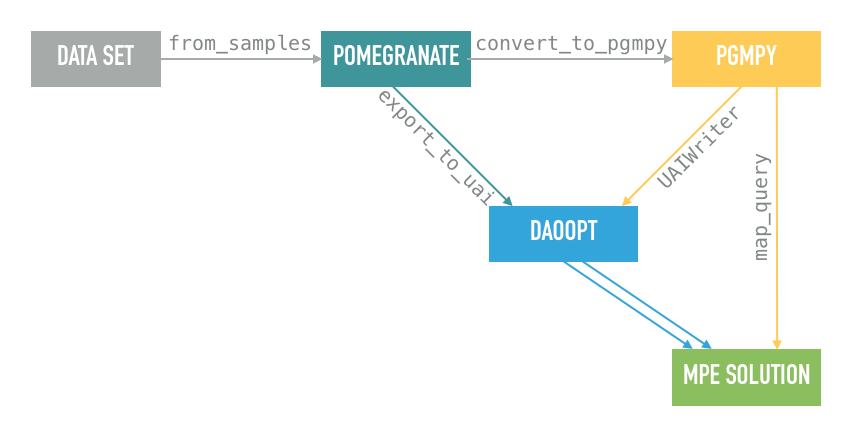
\includegraphics[width=\textwidth]{results/images/mpe_conversion_process}}
\caption{MPE calculation flow.}
\label{fig:mpe_conversion_process}
\end{figure}

The conversion from the Pomegranate-based to the Pgmpy-based model was thoroughly tested using conditional probability and independencies queries, so the issue is most likely to be found elsewhere.
As the DAOOPT MPE solution generated starting from the UAI differs from the one calculated directly with Pgmpy, there must be a bug either in Pgmpy's UAI exporter or in its inference method.
It is unclear if the following is still an issue (\url{https://github.com/pgmpy/pgmpy/issues/856}) but a series of test on simple networks, where the MPE calculation were carried out manually, seemed to confirm that \texttt{map\_query} was returning the correct MPE solution.

For example, in the small BN whose structure is shown in Figure \ref{fig:issues-bn} and the CPDs of the nodes in Tables \ref{tab:mut-cpd-issues}, \ref{tab:eta-cpd-issues}, \ref{tab:rec-cpd-issues} and \ref{tab:diff-cpd-issues}, Pgmpy's \texttt{map\_query} and DAOOPT returned different solutions to the following MPE query:
\begin{align}
\begin{split}
	\text{MPE}( \text{\enquote{differenziazione}}=x, \text{\enquote{mut17q21}}=y, \text{\enquote{recettori estrogeni}}=z \\
	\mid \text{\enquote{eta arrotondata}}=0 )
\end{split} 
\end{align}
\texttt{map\_query} returned the assignment: 
\begin{align} \label{eq:pgmpy-assignment}
  (\text{\enquote{differenziazione}}=1, 
  \text{\enquote{mut17q21}}=1, 
  \text{\enquote{recettori estrogeni}}=2)
\end{align}
while DAOOPT on the UAI exported with Pgmpy's returned:
\begin{align} \label{eq:daoopt-assignment}
  (\text{\enquote{differenziazione}}=0, 
  \text{\enquote{mut17q21}}=1, 
  \text{\enquote{recettori estrogeni}}=2)
\end{align}

In such a small network it is easy to verify that the probability of Equation \ref{eq:pgmpy-assignment} is: $0.99 \times 0.84 \times 0.60 = 0.50$ and that it is the MPE solution.
The fact that the probability of Equation \ref{eq:daoopt-assignment} is $0.99 \times 0.84 \times 0.21 = 0.17$, makes it obviously incorrect.

\begin{figure}[htbp]
\centerline{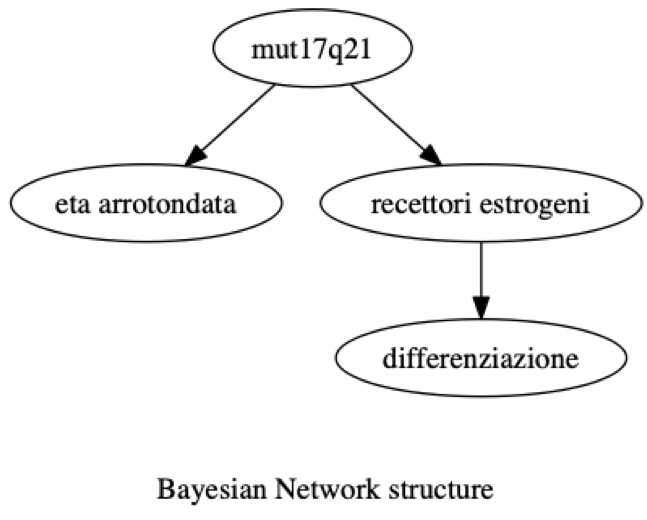
\includegraphics[width=0.5\textwidth]{results/images/issues-bn}}
\caption{Independencies query natural language output.}
\label{fig:issues-bn}
\end{figure}

\begin{table*}[htbp]
\centering
\caption{mut17q21 distribution}
\begin{tabularx}{\textwidth/3}{ccX}
\toprule
 \multirow{2}{*}{\textbf{mut17q21}} & 0 & 0.01  \\
 & 1 & 0.99 \\
\bottomrule
\end{tabularx}
\label{tab:mut-cpd-issues}
\end{table*}

\begin{table*}[htbp]
\centering
\caption{eta arrotondata CPT}
\begin{tabularx}{0.5\textwidth}{ccXX}
\toprule
      & &  \multicolumn{2}{c}{\textbf{mut17q21}} \\
\cmidrule(lr){3-4}
 & & 0 & 1    \\ 
 \multirow{3}{*}{\textbf{eta arr.}}  & 0 & 0.42 & 0.04  \\
 & 1 & 0.42 & 0.17    \\
 & 2 & 0.15 & 0.78 \\
\bottomrule
\end{tabularx}
\label{tab:eta-cpd-issues}
\end{table*}

\begin{table*}[htbp]
\centering
\caption{recettori estrogeni CPT}
\begin{tabularx}{0.5\textwidth}{ccXX}
\toprule
      & &  \multicolumn{2}{c}{\textbf{mut17q21}} \\
\cmidrule(lr){3-4}
 & & 0 & 1    \\ 
 \multirow{3}{*}{\textbf{rec. estr.}}  & 0 & 0.68 & 0.13  \\
 & 1 & 0.0 & 0.02    \\
 & 2 & 0.31 & 0.84 \\
\bottomrule
\end{tabularx}
\label{tab:rec-cpd-issues}
\end{table*}

\begin{table*}[htbp]
\centering
\caption{differenziazione CPT}
\begin{tabularx}{0.5\textwidth}{ccXXX}
\toprule
      & &  \multicolumn{3}{c}{\textbf{recettori estr.}} \\
\cmidrule(lr){3-5}
 & & 0 & 1 & 2   \\ 
 \multirow{3}{*}{\textbf{diff.}}  & 0 & 0.012 & 0.16 & 0.21  \\
 & 1 & 0.18 & 0.43 & 0.60    \\
 & 2 & 0.80 & 0.40 & 0.18 \\
\bottomrule
\end{tabularx}
\label{tab:diff-cpd-issues}
\end{table*}

\subsection{Late Removal of Clinical Variables} \label{subsec:removal-clinical-variables}
As discussed in Section \ref{sec:data-set}, some variables were chosen to be dropped from the initial data set.
Among these, \enquote{mut17q21}, \enquote{loss 17} and \enquote{FISHRatio} were initially included in the post-processed data set and became part of the Bayesian Network.
Thus, in the initial phases of development and validation the network topology was the one shown in Figure \ref{fig:old-bn-plot}, which can be compared with the current one shown in Figure \ref{fig:sw_plot_result}.

\begin{figure}[htbp]
\centerline{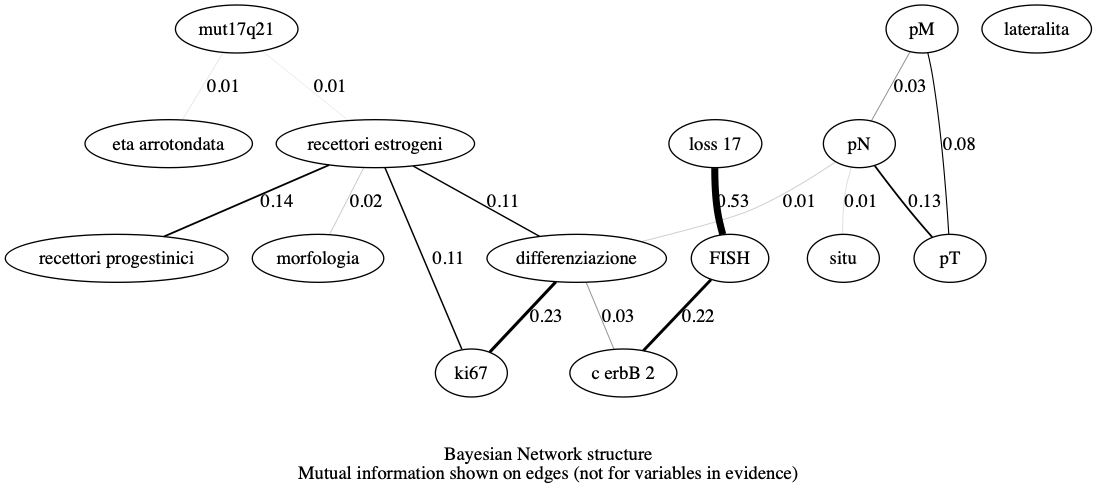
\includegraphics[width=\textwidth]{results/images/old-bn-plot}}
\caption{Bayesian Network topology before the removal of \enquote{mut17q21}, \enquote{loss 17} and \enquote{FISH}.}
\label{fig:old-bn-plot}
\end{figure}

At a later phase a decision was made, in concert with the ICP, to remove these three variables from the data set during the preprocessing phase; this on the basis of them being extremely skewed in their values, as can be seen by inspecting the \enquote{Distribution} column in Table \ref{tab:datasetdistribution}.

The reason for their skewness was briefly mentioned in Subsection \ref{subsec:motivation} and can be traced to the fact that these variables are all connected to the technique of Fluorescence in Situ Hybridisation (FISH).
This can be understood by analysing the \enquote{Clinical meaning} column in Table \ref{tab:datasetvariables} and knowing that FISH enables the analysis of specific DNA sequences on chromosomes and in particular of chromosome 17, because of its significance in breast cancer \citep{zhang2011important}.
FISH was a technique that was not available prior to 2010 and thus nearly 70\% of the patients in the data base had a value of \enquote{NCO} for \enquote{FISHRatio}, meaning this test had not been carried out on them.
Even worse, \enquote{mut17q21} presented more than 99\% \enquote{unknown} values and \enquote{loss 17} had 78\% of \enquote{FISH non fatta/FISH non valutabile}, meaning that the great majority of cases presented values with no real clinical meaning.

It can be seen in Figure \ref{fig:old-bn-plot} how strong the association between \enquote{loss 17} and \enquote{FISH} was - \textit{a posteriori}, a clear case of spurious correlation -, and how feebly \enquote{mut17q21} was connected to the rest of the network.
Leaving these variables thus introduced a very large amount of bias that confounded the resulting model.
An example of this effect was experienced in the early stages of validation; a previous series of validation questions had been prepared by the ICP and included queries in a form similar to:
\begin{quotation}
	In the general population, if \textit{[...]} is \textit{[...]}, then is it more/less probable that \textit{[...]} is \textit{[...]}?
\end{quotation}
and
\begin{quotation}
	In young patients, if \textit{[...]} is \textit{[...]}, then is it more/less probable that \textit{[...]} is \textit{[...]}?
\end{quotation}
Queries of these forms, when compared against each other, reliably returned identical answers thus indicating that the age of the patient (\enquote{eta arrotondata} in the benchmark data set) had little or no influence of the values of other variables.
Inspection of Figure \ref{fig:sw_plot_result} will show how, after the removal of \enquote{mut17q21}, \enquote{loss 17} and \enquote{FISHRatio}, \enquote{eta arrotondata} actually becomes disconnected from the rest of the network.
The removal of the spurious \enquote{bridge} created by \enquote{mut17q21} now explicitly shows and confirms that patient age can have no influence on other variables' values, as had already been noticed. 

The ICP confirmed that removing these three variables helped its users in better understanding the differences between a correlation in the variables representing the data set and a correlation in the actual clinical meaning behind the data.
That is, they felt that it reduced the \textit{confounding factors} thus allowing a better appreciation of the explainability method used.
\section{Summary}
This chapter has dealt with the outcomes of the work shown in Chapter \ref{chap:methodology}, that is the developed proof of concept software system which was used to validate the initial hypotheses regarding the explainability of Bayesian Network.

The implemented tool has been described and presented in detail by looking at every user interaction mode separately and at how these relate to the framework proposed by \citet{lacave2002review}.
Where present, the results of an \enquote{informal evaluation} of the system have been included; these are the result of observing and interacting personally with the ICP's experts.
The interaction modes analysed are:
\begin{itemize}
  \item \enquote{plot model}
  \item \enquote{independencies/d-separation query}
  \item \enquote{conditional probability query}
  \item \enquote{MPE query}
  \item \enquote{Pseudo-MPE query}
  \item three variant of \enquote{dialogue}
\end{itemize}

The first validation results that have been reported are those regarding the \textit{clinical validation} of the system as the outcome of these underpins the validity of all others.
The complete series of results to the natural language questions presented in Subsection \ref{subsec:clinical-validation-methodology} has been presented, together with the experts' comments.
The results, when summarised, confirm that the ICP considers the system's outputs clinically valid.
An extra discussion to better contextualise the clinical relevance of the system has also been included.

The evaluation of the system's explainability hinges on an \enquote{Explainability Evaluation Questionnaire}, a method borrowed from the Social Sciences, that was submitted to the ICP around three weeks after they had started using the software.
The questionnaire aims to disentangle the explainability of the single interaction modes and thus trace it back to more general explainability concepts for BNs.
The results seem to confirm that the system was indeed explainable, based on the warm reception it received by seasoned medical professionals, who had explicitly stated their aversion to having to deal with the inner workings of a ML tool.
The dialogue mode of interaction was appreciated in its novelty and potential to conduct clinical research, but was ultimately too deemed more onerous than other implemented approaches.
A novel result was that \textit{verbal} explanations were consistently rated more highly than \textit{visual} ones, contradicting finding in \citep{lacave2002review}.

Two evaluations have then been discussed for non-user-facing features: the first compared the quality of solution given by the \enquote{Pseudo-MPE} algorithm compared with the true MPE, the second assessed the power of the learned BN as a classifier against common Machine Learning methods.

The final section of the chapter has assessed the main issues encountered during the development and implementation of the methods in this thesis.
These include zero-valued entries in the Conditional Probability Tables learned by Pomegranate and the algorithm used to solve this problem, complications in the calculation of the true MPE solution using DAOOPT and Pgmpy and the effect that a late-stage removal of three variables from the data set had.

%%%%
%%%% CONCLUSIONS
%%%%
\chapter{Conclusions} \label{chap:conclusions}
\section{Discussion}
This thesis sets out as an investigation into the \textit{explainability} of Bayesian Networks.

The motivation leading to such a research question is to be found in the recent surge in the use of AI that is more and more integrated into the fabric of our society (see Section \ref{sec:intro-context}).
It has thus become imperative for these systems to be \textit{explainable}; that is, for its users to be able to understand the \textit{reasoning} behind the machine's outputs (see Section \ref{sec:explainability}).
This need is even more pressing in mission-critical domains such as that of Medicine.

The initial basis for the research carried out in this thesis has been the paper \citep{Butz2018} (see Section \ref{sec:explaining-the-most-probable-explanation}) that, while proposing a seemingly appealing method to enable the understanding of a medical data set, failed - as many other xAI works do - to provide any validation for its claims.
Thus a proof of concept system was developed\footnote{The complete source code is available at \url{https://github.com/Tioz90/Bayesian-Networks-Explainability-Tool}} in order to make an attempt at validating the claims made by the paper and, more in general, investigate the ability of Bayesian Networks to provide meaningful explanations to their users.
The benchmark against which the system's outputs have been compared are the \textit{explainability framework for BNs} offered by \citet{lacave2002review} and also the \textit{psychological characteristics inherent to an explanation} identified by \citet{miller2018explanation} (see Section  \ref{sec:explainability-in-bayesian-networks}).
One of the main gaps in the xAI literature has been the absence of real validation of the models being proposed by researchers, so among the main objectives of this thesis there was also to attempt to provide a methodological framework for the evaluation of machine learning systems with real domain experts i.e., an \textit{application-grounded evaluation} \citep{doshi2017towards} (see Section \ref{sec:evaluation-of-explainability}).

The prototype system was created by the implementation of standard techniques (see Subsection \ref{subsec:algorithms}) and the development of novel ones (see Subsection \ref{subsec:algorithms-novel}).
The underlying Bayesian Network was learned by using a real medical data set (see Section \ref{sec:data-set}).
This data set was provided by the medical partner, the Istituto Cantonale di Patologia in Locarno (Switzerland), who had a high degree of involvement at every step of this work (see Subsection \ref{subsec:istituto-cantonale}).
The expert pathologists at the ICP helped in both informing of the desiderata of the developed system but, most importantly, were crucial in validating it from a clinical relevance point of view and as regards its ability to interact meaningfully with them, that is they evaluated its \textit{explainability}.

The clinical relevance was evaluated by asking the ICP to define a series of natural language clinical questions that were then mapped onto the system's interaction modes (see Subsection \ref{subsec:clinical-validation-methodology} and \nameref{chap:annex}).
The results that the tool gave to these queries were compared by the experts at the ICP with those that they would have expected, based on medical literature and their personal expertise (see Subsection \ref{subsec:clinical-validation-results}).
In this respect, it has emerged that the tool, and the underlying BN, were able to capture and reply in a significant way to nearly all these questions thus validating it from a clinical relevance point of view.
This first validation step was important in order to establish a solid basis for the users to trust the system; if the system had not been able to implement the questions asked by the ICP or to offer them answers conforming to their expectations, it would have then been very difficult for it to then provide any meaningful explanation to the medical experts (see Section \ref{sec:importance-of-explainability}).
This because the users would not trust its outputs and, as discussed throughout Chapter \ref{chap:literature-review}, an explanation becomes such by virtue of a - sometimes metaphorical - dialogue between an \textit{explainer} (the machine) and an \textit{explainee} (the user).
If the two actors involved in an explanation are not able, or willing, to interface in a certain way, an explanation simply never comes into being.
The way - outputs, trust ... - in which humans and machines should interact in order for the former to explain something meaningful to the latter and the ways to elicit this interchange, is the focus of the Explainable AI field.

The evaluation of the explanatory powers of the tool was instead carried out by both an \textit{informal evaluation} (see Section \ref{sec:implemented-tool}), observing the experts using the tool and recording their impressions and issues, and a \textit{formal one} (see Subection \ref{subsec:explainability-validation} and \ref{subsec:explainability-validation-results}), involving an \enquote{Explainability Evaluation Questionnaire} (see \nameref{chap:annex}) geared towards probing the explainability of the system in the frameworks set by \citet{lacave2002review} and \citet{miller2018explanation}.
Both evaluations confirmed that the \textit{dialogical} explanation mode found in \citet{Butz2018} was the least effective means to offer the experts an explanation.
Thus, the claims made in the paper can not presently be substantiated by this thesis, but this result does obviously not disprove the explainability of Bayesian networks as a whole.
Another result, confirmed by both evaluations, was that the experts were very biased against preferring the \textit{verbal} explanation modality over any other; this seems to disprove the statement \enquote{the most direct and intuitive way of showing the information embodied in a Bayesian network is to display the corresponding graph} \citep{lacave2002review}.
If the explainability of Bayesian Networks is to be approximated in the satisfaction of the users of the system, then the work carried out in this thesis certainly seems to be a step in the direction of confirming the explanatory powers of such graphical models.
The experts of the ICP confirmed that they were able to interact meaningfully and fruitfully with the system and expressed the wish to continue using it on newer data sets.
The developed proof of concept system presented a mix of \textit{static} and \textit{dynamic} explanations together with \textit{contrastive}, \textit{linguistic} and \textit{visual} output modalities.
Even though the \enquote{dialogues}, that are instances of a \textit{dynamic}, \textit{contrastive}, \textit{linguistic} and \textit{visual} explanation, were not easy for the users to use meaningfully, the other explanatory modes like \enquote{MPE}, \enquote{pseudo-MPE} and \enquote{conditional probability queries} seemed to completely satisfy the experts at the ICP.
These other explanatory modes make use of one of the characteristics of BNs, namely that their outputs are \textit{selected}.
The results in this thesis thus seem to indicate that simple \textit{selection} of the outputs may be more important to medical users that the other characteristics - present in the \enquote{dialogues} and to a certain extent in \enquote{pseudo-MPE queries} - of explanations identified by \citet{miller2018explanation}: \textit{contrastiveness}, \textit{causality} and \textit{sociality}.

As regards laying out an \textit{evaluation methodology groundwork} for future \textit{application-based evaluations} of machine learning models in the medical domain, the hope is certainly to have done so fruitfully, barring the limitations recognised in Section \ref{sec:future-work}.
The evaluation methodology was able to surface results that were not in line with the established literature and thus these should surely merit further consideration.
Time was also included as part of this evaluation and this presents quite an element of novelty because, as noted by \citet{gilpin2018explaining}, this element is usually missing in xAI literature.
Nonetheless, many interesting results specific to the medical domain (reported throughout Chapter \ref{chap:results} where relevant) were surfaced through the application of the \textit{research methodology} and the resulting prototype system was also warmly received by its expert users.
Thus, one could certainly feel a certain degree of confidence in this research methodology being able to accurately characterise the domain of interest and to inform the building of effective \textit{explanatory tools} within it.
\section{Future Work} \label{sec:future-work}
When considering possible future work, one needs to distinguish between tasks whose scope is to \textit{address limitations of the current methods} and those related to \textit{expansion of the current work} and \textit{novel applications for it}.

\subsection{Addressing Limitations of Current Work}
\subsubsection{Methodology}
Based on the \enquote{formal} (see Subsection \ref{subsec:explainability-validation-results}) and \enquote{informal} (see Section \ref{sec:implemented-tool}) feedback received by the medical partner, it appears that the \enquote{dialogue} interaction modes (see Subsection \ref{subsec:dialogue-results}) should be modified, as the experts were not easily able to understand their workings, even after having perceived their potential.
The experts believed that with extra time they would have been able to use this interaction mode productively, but this is a symptom of a failure on the part of the software as a system designed to be explainable should definitively require as little effort from the user as possible.
The ICP has nonetheless confirmed its intention to continue using the software, focusing in particular on the dialogue modes of interaction, as they feel they have potential as research tools.
The evaluation methodology borrowed techniques from the social sciences but could undoubtedly be improved by experts in this domain, who will certainly be better versed in the methodological details compared to the author of this thesis, whose academic background is firmly in computer science.

\subsubsection{Additional Evaluations}
A more extended evaluation period could certainly be recommended as it would also enable the assessment of the effect of \textit{novelty} of certain interaction modes and help in factoring out the \textit{experts' preconceptions} regarding what an explanation should look like (see Subsection \ref{subsec:domain-experts-initial-expectations}).

The \enquote{pseudo-MPE} query also presented elements of ambiguity for the experts, as they were confused on the non-monotonicity of the probability of the elements in the deduction chain (see Subsection \ref{subsec:results-pseudo-mpe-query}).
This is unquestionably a point to investigate further by implementing and evaluating alternative \textit{output modalities}, as well as potentially \textit{linguistic} ones as these were proved to be preferred by the clinicians over all others.
The objective would be to identify the \textit{point of attrition} and discriminate if it were to be found in the actual underlying method or only in the way its outputs were displayed.
In the same vein, the reasons for the experts' misunderstanding in how to implement questions 23, 25, 27 on the system (see Section \ref{sec:results-validation-results}) should also be investigated more thoroughly.

\subsubsection{System}
The system developed in this thesis is bound by the limitations inherent to any proof of concept software, namely a general lack of polish and of somewhat lacking usability.
The methods themselves are studied to be able to surface explanations in the clearest way possible, but substituting the console-based frontend for a GUI - local or web-based - would beyond doubt lead to a marked improvement in the user experience.
Also related to the experimental nature of the software is the fact that it was not built from the start with a coherent end-goal but was extended in a non-organic manner as new methods were selected for exploration or novel ones were developed.
As a result the implementation presents some fragmentation and is rich in \enquote{workarounds}.
The choice of Python as the implementation language, while definitively advantageous for rapid development thanks to the comprehensive set of data science and machine learning libraries available, brought with it some clear limitations.
A Python application, while portable across different systems, does not provide a \textit{native} experience on any platform; the current project also relied heavily on the \textit{Anaconda} package manager\footnote{\url{https://www.anaconda.com}} so any user wishing to use the tool on their machine would need to deal with a potentially intricate setup process.
A better alternative to a full rewrite in a compiled language would be a web GUI to a Python backend\footnote{For example by using \url{https://github.com/epeios-q37/atlas-python}.} that would enable portability without requiring to completely change the implementation.
Nevertheless, a rewrite of the application that dropped many redundancies, unused code, and non-user-focused features, is a necessary part of future work.

\subsection{Extensions and Novel Applications}
The second class of future work concerns the expansion of the current techniques.
During this research it was not possible to utilise the software tool DAOOPT (see Subsection \ref{subsec:libraries} under the \enquote{DAOOPT} header) for exact MPE inferences and it was consequently not used as a benchmark for the \enquote{pseudo-MPE} algorithm (see Subsection \ref{subsec:results-mpe-calculation-issues}).
There is, however, a roadmap to follow up in more detail on the evaluation of the \enquote{pseudo-MPE} algorithm in a separate paper co-authored with IDSIA researchers.

One of the issues encountered in this thesis was the late removal of three variables due to their lack of clinical significance, as described in Subsection \ref{subsec:removal-clinical-variables}.
The ICP is in possession of a newer data set, homogeneous to the \textit{benchmark data set} used throughout this thesis (see Section \ref{sec:data-set}), where the values of two of the three variables (\enquote{FISH} and \enquote{loss17}) are defined and thus have clinical noteworthiness.
The third variable (\enquote{mut17q21}) is still missing too high a number of values to be relevant but these could be predicted using the BN or other discriminative ML techniques.
The estimation of the values of this last variable is bound to be accurate, as there is a real \textit{causal} dependency between it and the other two; this is because \enquote{mut17q21}, the mutation on chromosome 17, is identified through the technique of \textit{fluorescent in situ hybridisation} and is thus also tightly coupled with the results of \enquote{loss17}.
These are all novel clinical variables and they are thus open to being the subject of many research questions; the medical partner has confirmed its interest in using the tool developed in this thesis to pursue such investigations and this could, potentially, lead to scientific publications.

Connected to the previous point, the expert users suggested developing a \enquote{workflow} for the importing of new data sets, thus extending the clinical capabilities of the tool.
The experts also felt that the ability to save the textual and visual outputs of previous queries could undoubtedly be useful, together with the capacity to \enquote{snapshot} the state of a \enquote{dialogue} in order to resume it from a certain point onwards.
Ready-made query masks that could reduce the time needed to execute similar questions were also a request.

The ICP has also confirmed that it will be investigating the clinical relevance, through literature reviews and experiments, of some of the results obtained while using the tool; in particular, these would be those related to:
\begin{itemize}
  \item the lack of correlation between common clinical pathological features (i.e., morphology, TNM, grade, hormonal status) with age at diagnosis;
  \item the correlation between positive progesterone expression and low tumour proliferation index (ki67);
  \item the correlation between negative oestrogen receptor expression and high tumour proliferation index (ki67).
\end{itemize}

Finally, some interesting research avenues were not explored, for example a work by \citet{Kyrimi2016} who introduced a method that can be seen as the \enquote{inverse} of that proposed by \citet{Butz2018}.
Instead of looking for the outcome best explained by the given evidence, this other paper proposes techniques to find the evidence that best explains the chosen target variables.
Adapting this \enquote{inverse} method could potentially extend the \textit{explanatory powers} of the system, for example by enabling clinicians to understand which variables best justify a series of observed features in a patient.
It should not be too difficult an undertaking, as the current Python implementation is highly modular, by virtue of being based on standard open-source data structure libraries.

%%%%
%%%% CONCLUSIONS
%%%%
\appendix %optional, use only if you have an appendix

\backmatter

\chapter{Acronyms} \label{chap:acronyms} %optional
\chapter{Acronyms}
This first annex contains a list of acronyms used throughout this thesis, paired with the corresponding phrases of which they are the abbreviation.
Throughout the text, the acronym is usually paired with the phrase it refers to when first used.

\begin{itemize}
  \item \textbf{AI}: Artificial intelligence
  \item \textbf{API}: Application programming interface
  \item \textbf{BN}: Bayesian network
  \item \textbf{CPD}: Conditional probability distribution
  \item \textbf{CPT}: Conditional probability table
  \item \textbf{DAG}: Directed acyclic graph
  \item \textbf{EBNF}: Extended Backus-Naur form
  \item \textbf{FISH}: Fluorescence in situ hybridisation
  \item \textbf{GDPR}: General Data Protection Regulation
  \item \textbf{GUI}: Graphical user interface
  \item \textbf{ICP}: Istituto Cantonale di Patologia
  \item \textbf{IDSIA}: Dalle Molle Institute for Artificial Intelligence
  \item \textbf{MAP}: Maximum a posteriori
  \item \textbf{ML}: Machine learning
  \item \textbf{MLE}: Maximum likelihood estimation
  \item \textbf{MPE}: Most probable explanation
%  \item \textbf{SVM}: Support vector machine
  \item \textbf{xAI}: Explainable artificial intelligence
%  \item \textbf{LDA}: Linear discriminant analysis
\end{itemize}

\chapter{Annex} \label{chap:annex}
\newcounter{annexcounter}

\begin{sidewaystable*}[h]
  \centering
  \captionsetup{name=Annex}
  \caption{Natural language questions that can be answered by conditional probability queries}
    \begin{tabularx}{\textwidth}{lXllllX}
	    \toprule
	    \textbf{\#} & Natural language question & Type  & Target variable & Target value & Evidence variable & Evidence value \\
		\midrule
		\textbf{1} & At diagnosis, if estrogen receptors are negative, is tumor proliferative index high? & validation & ki67  & >30\% & estrogeni & 0-10\% \\
		\addlinespace
		\textbf{2} & At diagnosis, if estrogen receptors are negative, is the risk of metastases low? & validation & pM sub & pM=0  & estrogeni & 0-10\% \\
		\addlinespace
		\multirow{2}[0]{*}{\textbf{3}} & \multirow{2}[0]{4cm}{If estrogen receptors are negative and tumor proliferative index is  high at diagnosis, is the risk of metastases low?} & \multirow{2}[0]{*}{validation} & \multirow{2}[0]{*}{pM sub} & \multirow{2}[0]{*}{pM=0} & estrogeni & 0-10\% \\
		      &       &       &       &       & ki67  & >30\% \\
		\addlinespace[9ex]
	      \textbf{4} & If the diagnosis of mammary carcinoma happened at a young age, is tumour proliferative index high? & validation/research & ki67  & >30\% & eta arrotondata & <40 \\
      	\addlinespace
		\textbf{5} & If the histologic diagnosis is of lobular carcinoma, is the expression of the c-erbB2 marker absent? & validation & cerb  & 0 \& 1 & morfologia & Lobular carcinoma, NOS \\
		\addlinespace
		\textbf{6} & If the tumour is large, is lymph node involvement more probable? & validation & pN sub & pN!=0 & pT sub & pT>=2  \\  
		\addlinespace[2ex]
		\multirow{2}[0]{*}{\textbf{7}} & \multirow{2}[0]{4cm}{If the tumour is large and lymph nodes are involved, is the risk of metastases low at diagnosis?} & \multirow{2}[0]{*}{validation} & \multirow{2}[0]{*}{pM sub} & \multirow{2}[0]{*}{pM=0} & pT sub & pT>=2  \\ 
		&       &       &       &       & pN sub & pN!=0 \\  
\end{tabularx}
	\refstepcounter{annexcounter}
	\label{ann:conditionalprobability1}
\end{sidewaystable*}

\begin{sidewaystable*}[h]
  \centering
  \captionsetup{name=Annex}
  \caption{Natural language questions that can be answered by conditional probability queries}
    \begin{tabularx}{\textwidth}{lXllllX}
	    \toprule
	    \textbf{\#} & Natural language question & Type  & Target variable & Target value & Evidence variable & Evidence value \\
		\midrule      
		\textbf{8} & If the tumour is of high grade at diagnosis, is the risk of metastases low? & validation & pM sub & pM=0  & differenziazione & poco differenziato \\
		\multirow{2}[0]{*}{\textbf{9}} & \multirow{2}[0]{4cm}{In young patients, if estrogen receptors are negative, is tumor proliferative index high?} & \multirow{2}[0]{*}{validation} & \multirow{2}[0]{*}{ki67} & \multirow{2}[0]{*}{>30\%} & estrogeni & 0-10\% \\
		      &       &       &       &       & eta arrotondata & <40 \\	  
	    \addlinespace[6ex]
		\multirow{2}[0]{*}{\textbf{10}} & \multirow{2}[0]{4cm}{In young patients, if estrogen receptors are negative, is the risk of metastases low?} & \multirow{2}[0]{*}{validation} & \multirow{2}[0]{*}{pM sub} & \multirow{2}[0]{4cm}{pM=0} & estrogeni & 0-10\% \\
		      &       &       &       &       & eta arrotondata & <40 \\
      \addlinespace[6ex]
		\multirow{3}[0]{*}{\textbf{11}} & \multirow{3}[0]{4cm}{In young patients, if estrogen receptors are negative and tumor proliferative index is  high at diagnosis, is the risk of metastases low?} & \multirow{3}[0]{*}{validation} & \multirow{3}[0]{*}{pM sub} & \multirow{3}[0]{*}{pM=0} & estrogeni & 0-10\% \\
		      &       &       &       &       & ki67  & >30\% \\
		      &       &       &       &       & eta arrotondata & <40 \\
      \addlinespace[9ex]
	      \multirow{3}[0]{*}{\textbf{12}} & \multirow{3}[0]{4cm}{How does the tumoural grade change if I know the oestrogen expression?} & \multirow{3}[0]{*}{research} & \multirow{3}[0]{*}{differenziazione} &  ben differenziato & \multirow{3}[0]{*}{estrogeni} & negativi (0-10\%) \\
		      &       &       &       &  moderatamente differenziato &       & debolmente positivo (10-50\%) \\
		      &       &       &       &  poco differenziato &       & fortemente positivo (>50\%) \\
	      \addlinespace[1ex]
		\multirow{4}[0]{*}{\textbf{13}} & \multirow{4}[0]{4cm}{How does the oestrogen expression change if I know the proliferation index?} & \multirow{4}[0]{*}{research} & \multirow{4}[0]{*}{estrogeni} &  negativi (0-10\%) & \multirow{4}[0]{*}{ki67} & negativo (0-14\%) \\
		      &       &       &       &  debolmente positivi (10-50\%) &       & 14-20\% \\
		      &       &       &       & \multirow{2}[0]{*}{fortemente positivi (>50\%)} &       & 20-30\% \\
		      &       &       &       &       &       & positivi (>30\%) \\
      \addlinespace[1ex]
	      \textbf{14} & Does the negative expression of progestinic receptors influence lymph nodes' state? & validation & pN sub & pN!=0  & progestinici & 0-10\% \\
      \end{tabularx}
	\refstepcounter{annexcounter}
	\label{ann:conditionalprobability2}
\end{sidewaystable*}

\begin{sidewaystable}[h]
	\centering
	\captionsetup{name=Annex}
	\caption{Natural language questions that can be answered by d-separation queries}
	\begin{tabularx}{\textwidth}{lXllllX}
		\toprule
		\textbf{\#} & Natural language question & Type  & Target variable & Target value & Evidence variable & Evidence value \\
		\midrule
		\textbf{14} & Which clinical-pathological variables influence the lymph nodes' state at diagnosis? & research & pN    & -     & -     & - \\
		\textbf{15} & Which clinical-pathological variables influence tumoural proliferation index? & research & ki67  & -     & -     & - \\
		\textbf{16} & Which clinical-pathological variables influence the expression of the c-ERBB2 marker? & research & cerb  & \multicolumn{1}{r}{} & -     & - \\
		\textbf{17} & Which clinical-pathological variables influence the oestrogen expression? & research & recettori estrogeni & \multicolumn{1}{r}{} & -     & - \\
		\textbf{18} & Which clinical-pathological variables influence the tumoural grade? & research & differenziazione & \multicolumn{1}{r}{} & -     & - \\
		\textbf{19} & Which clinical-pathological variables influence the presence of metastases at diagnosis? & research & pM    & \multicolumn{1}{r}{} & -     & - \\
		\textbf{20} & Which clinical-pathological variables influence the tumoural dimension? & research & pT    & \multicolumn{1}{r}{} & -     & - \\
		\textbf{21} & Which clinical-pathological variables influence the age of the tumour onset? & research & eta   & -     & -     & - \\
		\end{tabularx}
	\refstepcounter{annexcounter}
	\label{ann:dseparation}
\end{sidewaystable}

\begin{sidewaystable}[h]
	\centering
	\captionsetup{name=Annex}
	\caption{Natural language questions that can be answered by conditional probability queries or, at a higher level, by d-separation queries}
	\begin{tabularx}{\textwidth}{lXllllX}
		\toprule
		\textbf{\#} & Natural language question & Type  & Target variable & Target value & Evidence variable & Evidence value \\
		\midrule
		\multirow{2}[0]{*}{\textbf{22}} & \multirow{2}[0]{4cm}{In young patients, does a negative expression of the progestinic receptors influence the lymph nodes' state?} & \multirow{2}[0]{*}{research} & \multirow{2}[0]{*}{pN sub} & \multirow{2}[0]{*}{pN!=0} & progestinici & 0-10\% \\
	      &       &       &       &       & eta   & <40 \\
	      \addlinespace[9ex]
		\multicolumn{1}{r}{\textbf{23}} & Does a negative expression of progestinic receptors influence the tumoural proliferation index? & research & ki67  & >30\% & progestinici & 0-10\% \\
		\addlinespace
		\multirow{2}[0]{*}{\textbf{24}} & \multirow{2}[0]{4cm}{In young patients, does a negative expression of the progestinic receptors influence the tumoural proliferation index?} & \multirow{2}[0]{*}{research} & \multirow{2}[0]{*}{ki67} & \multirow{2}[0]{*}{>30\%} & progestinici & 0-10\% \\
		      &       &       &       &       & eta   & <40 \\
		      \addlinespace[10ex]
		\multirow{3}[0]{*}{\textbf{25}} & \multirow{3}[0]{4cm}{Does a negative expression of progestinic receptors influence the expression of the c-ERBB2 marker?} & \multirow{3}[0]{*}{research} & \multirow{3}[0]{*}{cerb} & 0 \& 1 & \multirow{3}[0]{*}{progestinici} & \multirow{3}[0]{*}{0-10\%} \\
		      &       &       &       & 2     &       &  \\
		      &       &       &       & 3     &       &  \\
		      \addlinespace[4ex]
		\multirow{4}[0]{*}{\textbf{26}} & \multirow{4}[0]{4cm}{In young patients, does a negative expression of the progestinic receptors influence the expression of the c-ERBB2 marker?} & \multirow{4}[0]{*}{research} & \multirow{4}[0]{*}{cerb} & 0 \& 1 & \multirow{3}[0]{*}{progestinici} & \multirow{3}[0]{*}{0-10\%} \\
		      &       &       &       & 2     &       &  \\
		      &       &       &       & \multirow{2}[0]{*}{3} &       &  \\
		      &       &       &       &       & eta   & <40 \\
		\end{tabularx}
	\refstepcounter{annexcounter}
	\label{ann:conditionalanddseparation}
\end{sidewaystable}

\begin{sidewaystable}[h]
	\centering
	\captionsetup{name=Annex}
	\caption{Natural language questions that can be answered by MPE queries}
	\begin{tabularx}{\textwidth}{lXllllX}
		\toprule
		\textbf{\#} & Natural language question & Type  & Target variable & Target value & Evidence variable & Evidence value \\
		\midrule
		\multirow{3}[0]{*}{\textbf{27}} & \multirow{3}[0]{4cm}{How are tumours characterised by a triple negative profile from the point of view of the other clinical-pathological variables?} & \multirow{3}[0]{*}{research} & \multirow{3}[0]{*}{-} & \multirow{3}[0]{*}{-} & cerb  & 0 \\
		\addlinespace[9ex]
	      &       &       &       &       & recettori estrogeni & negativo \\
	      &       &       &       &       & recettori progestinici & negativo \\
		\textbf{28} & How are tumours characterised by high ki67 from the point of view of the other clinical-pathological variables? & research & -     & -     & ki67  & >30 \\
		\addlinespace[2ex]
		\textbf{29} & How are tumours characterised by nodes involvement from the point of view of the other clinical-pathological variables? & research & -     & -     & pN    & !0 \\
		\end{tabularx}
	\refstepcounter{annexcounter}
	\label{ann:mpe}
\end{sidewaystable}

\begin{framed}
	\begin{center}
		{\huge Explainability evaluation questionnaire}
	\end{center}
	{\Large Confidence}
	\begin{enumerate} 
		\item Did the tool increase the confidence in diagnosis when diagnostic screening results were missing for a patient?  Why? \\
		O Yes O No
		\item Did the tool help in characterising a particular patient's profile? \\
		O Not at all O Somewhat O Absolutely
		\item Did the tool help in your confidence of understanding the cohort characteristics?  How? \\
		O Not at all O Somewhat O Absolutely
		\item Did the tool improve your confidence in your clinical decision-making?  How? \\ 
		O Not at all O Somewhat O Absolutely
		\item Did having the tool at your disposal improve your confidence when making time-constrained decisions?  How? (for example, did it improve confidence in prioritising some tests over others?) \\
		O Not at all O Somewhat O Absolutely
	\end{enumerate}
	{\Large Features}
	\begin{enumerate}[resume]
		\item Given the modes of interaction with the system labelled as \enquote{dialogues}, do you think you would have had more difficulty in interpreting the data without the these modalities? \\
		O No O Maybe O Yes
		\item Was natural language useful during the interaction?  Why? \\
		O No O Maybe O Yes
		\item Which type of \enquote{dialogue} did you feel was most useful? Why? \\
		O Exhaustive O Separations O Thresholded O A combination of the previous O All O None
		\item Did you feel that the dialogue helped you in cases of uncertainty?  If yes, how?  If no, why? \\
		O No O Somewhat O Yes
		\item Did you feel that the \enquote{dialogue} helped your clinical decision-making?  If yes, how?  If no, why? \\
		O No O Somewhat O Yes
		\item Did the generation of \enquote{counterfactual branches} help in your understanding of the data?  Why? \\
		O No O Somewhat O Yes
		\item Given the interaction mode labelled \enquote{Pseudo-MPE query}, how would you rate the solutions it proposed from a point of view of their understandability? (1 poor, 5 good) \\
		O 1 O 2 O 3 O 4 O 5
		\item How would you rate the Pseudo-MPE solutions from a point of view of their clinical usefulness? \\
		O 1 O 2 O 3 O 4 O 5
		\item Do you feel that the interaction mode labelled as \enquote{MPE query} gave better solutions than that labelled \enquote{Pseudo-MPE query}?  Why? \\
		O No O Maybe O Yes
		\item Did you find the \enquote{Pseudo-MPE} or \enquote{MPE} interaction mode the most useful?  Why? \\
		O Pseudo-MPE O MPE O Both O None
		\item How important was the highlighting of the independencies between variables? \\
		O 1 O 2 O 3 O 4 O 5
		\item Do you think you would have had more difficulty in interpreting the data without the correlation strength displayed? \\
		O No O Maybe O Yes
		\item Do you think you would have had more difficulty in interpreting the data without visualisations? \\
		O No O Maybe O Yes
		\item Do you think you would have had more difficulty in interpreting the data without natural language output? \\
		O No O Maybe O Yes
	\end{enumerate}
	{\Large Time}
	\begin{enumerate}[resume]
		\item How would you rate the time it took to understand the dialogues' outputs?  Which of the three was best? (1 bad, 5 good) \\
		O 1 O 2 O 3 O 4 O 5
		\item How would you rate the time it took to understand the conditional probability query's outputs \\
		O 1 O 2 O 3 O 4 O 5
		\item How would you rate the time it took to understand the MPE and Pseudo-MPE query's outputs? \\
		O 1 O 2 O 3 O 4 O 5
		\item Did natural language help in reducing the time needed to understand the outputs? \\
		O No O Somewhat O Yes
		\item Did visualisations help in reducing the time needed to understand the outputs? \\
		O No O Somewhat O Yes
	\end{enumerate}
	{\Large Tool}
	\begin{enumerate}[resume]
		\item Which interaction modes did you feel could be the most useful?  Why? \\
		O Plot model O Independencies O Conditional Probability Query O Pseudo-MPE and MPE O Dialogues
		\item Which interaction modes did you use the most?  Why? \\
		O Plot model O Independencies O Conditional Probability Query O Pseudo-MPE and MPE O Dialogues
		\item How did you use the tool in your day-to-day work?
		\item Is the tool missing any functionality that would address your needs?  If yes, which ones? \\
		O No O Yes
		\item Did you have any difficulties in understanding which functionalities to use to address your needs?  If yes, when? \\
		O No O Yes
		\item Did you have any difficulties in understanding the functionalities during usage?  If yes, when? \\
		O No O Yes
		\item If you answered Yes to the previous question, how do you think this could be addressed?
		\item Could you suggest any functionalities you would like to be implemented?
	\end{enumerate}
	{\Large Clinical}
	\begin{enumerate}[resume]
		\item Did the tool help in recovering missing features of patients thus supporting diagnostic profile creation and decision making? If yes, which is/are the feature/s that benefited the most? \\
		O No O Yes
		\item Did any of the tool's predictions have clinical confirmation later on?  If yes, how? \\
		O No O Yes
		\item Did the tool help in highlighting new relationships between variables? \\
		O No O Yes
		\item Did the tool help in highlighting new patient subgroups? \\
		O No O Yes
	\end{enumerate}
	{\Large Satisfaction}
	\begin{enumerate}[resume]
		\item What is your general satisfaction with the tool? For what reasons? \\
		O Completely dissatisfied O Somewhat dissatisfied O Neutral O Somewhat satisfied O Completely satisfied
	\end{enumerate}
	\refstepcounter{annexcounter}
	\label{ann:questionnaire}
\end{framed}




%\bibliographystyle{alpha}
%\bibliographystyle{dcu}
\bibliographystyle{plainnat}
\bibliography{biblio}

%\cleardoublepage
%\theindex %optional, use only if you have an index, must use
	  %\makeindex in the preamble


\end{document}
